\documentclass{article}
\usepackage[utf8]{inputenc}
\usepackage{amsmath,amsthm,amssymb,marvosym,mathrsfs,amsfonts,amscd, mathtools}
\usepackage[margin=2.5cm,headsep=0.5cm]{geometry}

% Hyperlink shit
\usepackage{hyperref}
\hypersetup{
    colorlinks,
    citecolor=black,
    filecolor=black,
    linkcolor=black,
    urlcolor=black
}

% Colors
\usepackage{xcolor}

% Nice frames
\usepackage{mdframed}

% Wrap figures
\usepackage{wrapfig}

% Bra Ket Notation
\usepackage{braket}

% Clean SI Units
\usepackage{siunitx}

\usepackage{enumitem}

% Cancel things out in equations
\usepackage[makeroom]{cancel}

% Better support for graphics and figures
\usepackage{graphicx}
\usepackage{wrapfig}
\usepackage{float}

% Highlighting
\usepackage{color,soul}

% Caption figures and tables
\usepackage{caption}

% Subfigures
\usepackage{subcaption}

% Generate symbols
\usepackage{textcomp} % Include this line to avoid output errors
\usepackage{gensymb}

\usepackage{relsize}

% Make multiple rows in a table
\usepackage{booktabs}
\usepackage{multirow}

% Big integerals
\usepackage{bigints}

% Asymptote
\usepackage{asymptote}
%\usepackage{parskip}

% < Tikz Package Shit>

\usepackage{pgf,tikz,pgfplots}
\usepackage{tikz-3dplot}
\usetikzlibrary{decorations.pathmorphing,patterns}
\usetikzlibrary{decorations.markings}
\pgfplotsset{compat=1.15}
\usetikzlibrary{arrows}
\usetikzlibrary{calc}
\usetikzlibrary{scopes}
\usetikzlibrary{angles, quotes}
\usetikzlibrary{svg.path}
\usetikzlibrary{arrows}
\usetikzlibrary{quotes,arrows.meta}
\usetikzlibrary{fadings,decorations.pathreplacing}

% Circled numbers that don't look like a shit
\newcommand*\circled[1]{\tikz[baseline=(char.base)]{
            \node[shape=circle,draw,inner sep=2pt] (char) {#1};}}

% < / Tikz Package Shit>

% pst
\usepackage{pstricks}
\usepackage{pst-electricfield}

% Blackboard bold shit
\usepackage{bm}
\DeclareSymbolFont{bbold}{U}{bbold}{m}{n}
\DeclareSymbolFontAlphabet{\mathbbold}{bbold}


\setlength{\parindent}{0pt}
\DeclarePairedDelimiter\floor{\lfloor}{\rfloor}
\newcommand{\bbN}{\mathbb{N}}
\newcommand{\bbZ}{\mathbb{Z}}
\newcommand{\bbR}{\mathbb{R}}
\newcommand{\bbQ}{\mathbb{Q}} 
\newcommand{\bbI}{\mathbb{I}}
\newenvironment{theorem}[2][Theorem]{\begin{trivlist}
\item[\hskip \labelsep {\bfseries #1}\hskip \labelsep {\bfseries #2.}]}{\end{trivlist}}
\newenvironment{lemma}[2][Lemma]{\begin{trivlist}
\item[\hskip \labelsep {\bfseries #1}\hskip \labelsep {\bfseries #2.}]}{\end{trivlist}}
\newenvironment{exercise}[2][Exercise]{\begin{trivlist}
\item[\hskip \labelsep {\bfseries #1}\hskip \labelsep {\bfseries #2.}]}{\end{trivlist}}
\newenvironment{reflection}[2][Reflection]{\begin{trivlist}
\item[\hskip \labelsep {\bfseries #1}\hskip \labelsep {\bfseries #2.}]}{\end{trivlist}}
\newenvironment{proposition}[2][Proposition]{\begin{trivlist}
\item[\hskip \labelsep {\bfseries #1}\hskip \labelsep {\bfseries #2.}]}{\end{trivlist}}
\newenvironment{corollary}[2][Corollary]{\begin{trivlist}
\item[\hskip \labelsep {\bfseries #1}\hskip \labelsep {\bfseries #2.}]}{\end{trivlist}}
\renewcommand\qedsymbol{$\blacksquare$}


% Number equations within sections
\numberwithin{equation}{section}

% Epigraphs
\usepackage{epigraph}

% Code listing
\usepackage{listings}
\definecolor{green_comments}{HTML}{00BA00}
\definecolor{gray_numbers}{HTML}{4F4F4F}
\definecolor{purple_strings}{HTML}{AD00AA}
\definecolor{background_color}{HTML}{E8E8E8}
\lstdefinestyle{kostin}{
    backgroundcolor=\color{background_color},   
    commentstyle=\color{green_comments},
    keywordstyle=\color{blue},
    numberstyle=\tiny\color{gray_numbers},
    stringstyle=\color{purple_strings},
    basicstyle=\footnotesize,
    breakatwhitespace=false,         
    breaklines=true,                 
    captionpos=b,                    
    keepspaces=true,                 
    numbers=left,                    
    numbersep=5pt,                  
    showspaces=false,                
    showstringspaces=false,
    showtabs=false,                  
    tabsize=2
}
\lstset{style=kostin}

% Unit basis vectors
\newcommand{\ihat}{\mathbf{\hat{i}}}
\newcommand{\jhat}{\mathbf{\hat{j}}}
\newcommand{\khat}{\mathbf{\hat{k}}}
\newcommand{\xhat}{\mathbf{\hat{x}}}
\newcommand{\yhat}{\mathbf{\hat{y}}}
\newcommand{\zhat}{\mathbf{\hat{z}}}
\newcommand{\rhat}{\mathbf{\hat{r}}}
\newcommand{\nhat}{\mathbf{\hat{n}}}
\newcommand{\ehat}{\mathbf{\hat{e}}}
\newcommand{\phihat}{\skew{3}{\hat}{\skew{3}{}{\bm{\phi}}}}
\newcommand{\thetahat}{\skew{3}{\hat}{\skew{3}{}{\bm{\theta}}}}

% Colors
\definecolor{ao}{HTML}{6F0EED}
\definecolor{DARK_BLUE}{HTML}{040080}
\definecolor{DARK_BROWN}{HTML}{8B4513}
\definecolor{LIGHT_BROWN}{HTML}{CD853F}
\definecolor{BLUE_E}{HTML}{1C758A}
\definecolor{BLUE_D}{HTML}{29ABCA}
\definecolor{BLUE_C}{HTML}{58C4DD}
\definecolor{BLUE_B}{HTML}{9CDCEB}
\definecolor{BLUE_A}{HTML}{C7E9F1}
\definecolor{TEAL_E}{HTML}{49A88F}
\definecolor{TEAL_D}{HTML}{55C1A7}
\definecolor{TEAL_C}{HTML}{5CD0B3}
\definecolor{TEAL_B}{HTML}{76DDC0}
\definecolor{TEAL_A}{HTML}{ACEAD7}
\definecolor{GREEN_E}{HTML}{699C52}
\definecolor{GREEN_D}{HTML}{77B05D}
\definecolor{GREEN_C}{HTML}{83C167}
\definecolor{GREEN_B}{HTML}{A6CF8C}
\definecolor{GREEN_A}{HTML}{C9E2AE}
\definecolor{YELLOW_E}{HTML}{E8C11C}
\definecolor{YELLOW_D}{HTML}{F4D345}
\definecolor{YELLOW_C}{HTML}{FFFF00}
\definecolor{YELLOW_B}{HTML}{FFEA94}
\definecolor{YELLOW_A}{HTML}{FFF1B6}
\definecolor{GOLD_E}{HTML}{C78D46}
\definecolor{GOLD_D}{HTML}{E1A158}
\definecolor{GOLD_C}{HTML}{F0AC5F}
\definecolor{GOLD_B}{HTML}{F9B775}
\definecolor{GOLD_A}{HTML}{F7C797}
\definecolor{RED_E}{HTML}{CF5044}
\definecolor{RED_D}{HTML}{E65A4C}
\definecolor{RED_C}{HTML}{FC6255}
\definecolor{RED_B}{HTML}{FF8080}
\definecolor{RED_A}{HTML}{F7A1A3}
\definecolor{MAROON_E}{HTML}{94424F}
\definecolor{MAROON_D}{HTML}{A24D61}
\definecolor{MAROON_C}{HTML}{C55F73}
\definecolor{MAROON_B}{HTML}{EC92AB}
\definecolor{MAROON_A}{HTML}{ECABC1}
\definecolor{PURPLE_E}{HTML}{644172}
\definecolor{PURPLE_D}{HTML}{715582}
\definecolor{PURPLE_C}{HTML}{9A72AC}
\definecolor{PURPLE_B}{HTML}{B189C6}
\definecolor{PURPLE_A}{HTML}{CAA3E8}
\definecolor{WHITE}{HTML}{FFFFFF}
\definecolor{BLACK}{HTML}{000000}
\definecolor{LIGHT_GRAY}{HTML}{BBBBBB}
\definecolor{GRAY}{HTML}{888888}
\definecolor{DARK_GRAY}{HTML}{444444}
\definecolor{DARKER_GRAY}{HTML}{222222}
\definecolor{GRAY_BROWN}{HTML}{736357}
\definecolor{PINK}{HTML}{D147BD}
\definecolor{LIGHT_PINK}{HTML}{DC75CD}
\definecolor{GREEN_SCREEN}{HTML}{00FF00}
\definecolor{ORANGE}{HTML}{FF862F}

\newcommand{\DARKBLUE}{\color{DARK_BLUE}}
\newcommand{\DARKBROWN}{\color{DARK_BROWN}}
\newcommand{\LIGHTBROWN}{\color{LIGHT_BROWN}}
\newcommand{\BLUEE}{\color{BLUE_E}}
\newcommand{\BLUED}{\color{BLUE_D}}
\newcommand{\BLUEC}{\color{BLUE_C}}
\newcommand{\BLUEB}{\color{BLUE_B}}
\newcommand{\BLUEA}{\color{BLUE_A}}
\newcommand{\TEALE}{\color{TEAL_E}}
\newcommand{\TEALD}{\color{TEAL_D}}
\newcommand{\TEALC}{\color{TEAL_C}}
\newcommand{\TEALB}{\color{TEAL_B}}
\newcommand{\TEALA}{\color{TEAL_A}}
\newcommand{\GREENE}{\color{GREEN_E}}
\newcommand{\GREEND}{\color{GREEN_D}}
\newcommand{\GREENC}{\color{GREEN_C}}
\newcommand{\GREENB}{\color{GREEN_B}}
\newcommand{\GREENA}{\color{GREEN_A}}
\newcommand{\YELLOWE}{\color{YELLOW_E}}
\newcommand{\YELLOWD}{\color{YELLOW_D}}
\newcommand{\YELLOWC}{\color{YELLOW_C}}
\newcommand{\YELLOWB}{\color{YELLOW_B}}
\newcommand{\YELLOWA}{\color{YELLOW_A}}
\newcommand{\GOLDE}{\color{GOLD_E}}
\newcommand{\GOLDD}{\color{GOLD_D}}
\newcommand{\GOLDC}{\color{GOLD_C}}
\newcommand{\GOLDB}{\color{GOLD_B}}
\newcommand{\GOLDA}{\color{GOLD_A}}
\newcommand{\REDE}{\color{RED_E}}
\newcommand{\REDD}{\color{RED_D}}
\newcommand{\REDC}{\color{RED_C}}
\newcommand{\REDB}{\color{RED_B}}
\newcommand{\REDA}{\color{RED_A}}
\newcommand{\MAROONE}{\color{MAROON_E}}
\newcommand{\MAROOND}{\color{MAROON_D}}
\newcommand{\MAROONC}{\color{MAROON_C}}
\newcommand{\MAROONB}{\color{MAROON_B}}
\newcommand{\MAROONA}{\color{MAROON_A}}
\newcommand{\PURPLEE}{\color{PURPLE_E}}
\newcommand{\PURPLED}{\color{PURPLE_D}}
\newcommand{\PURPLEC}{\color{PURPLE_C}}
\newcommand{\PURPLEB}{\color{PURPLE_B}}
\newcommand{\PURPLEA}{\color{PURPLE_A}}
\newcommand{\WHITE}{\color{WHITE}}
\newcommand{\BLACK}{\color{BLACK}}
\newcommand{\LIGHTGRAY}{\color{LIGHT_GRAY}}
\newcommand{\GRAY}{\color{GRAY}}
\newcommand{\DARKGRAY}{\color{DARK_GRAY}}
\newcommand{\DARKERGRAY}{\color{DARKER_GRAY}}
\newcommand{\GRAYBROWN}{\color{GRAY_BROWN}}
\newcommand{\PINK}{\color{PINK}}
\newcommand{\LIGHTPINK}{\color{LIGHT_PINK}}
\newcommand{\GREENSCREEN}{\color{GREEN_SCREEN}}
\newcommand{\ORANGE}{\color{ORANGE}}
%\newcommand{\blue}{\color{blue}}
%\newcommand{\red}{\color{red}}
%\newcommand{\black}{\color{black}}

% Make math big
\newcommand*{\Scale}[2][4]{\scalebox{#1}{\ensuremath{#2}}}

% Evaluate expression - useful for integrals
\newcommand*\Eval[3]{\left.#1\right\rvert_{#2}^{#3}}

% Griffiths script r
\usepackage{calligra}
\DeclareMathAlphabet{\mathcalligra}{T1}{calligra}{m}{n}
\DeclareFontShape{T1}{calligra}{m}{n}{<->s*[2.2]callig15}{}
\newcommand{\scripty}[1]{\ensuremath{\mathcalligra{#1}}}


% Bunny. In honor of Dr. Pat Kohl.
\newcommand{\bunny}[1][]{
    \tikz \fill [scale=1ex/500,yscale=1,#1] svg "M3831 8683 c-70 -71 -235 -358 -326 -567 -168 -385 -252 -748 -275 -1181 -5 -104 -9 -199 -7 -209 2 -16 -10 -21 -88 -36 -158 -31 -407 -112 -530 -173 -117 -58 -239 -150 -365 -277 -178 -177 -305 -366 -407 -604 -44 -102 -55 -118 -136 -201 -110 -113 -148 -183 -154 -288 -4 -53 0 -88 14 -132 12 -37 16 -70 12 -85 -4 -14 -7 -62 -8 -107 -3 -225 125 -386 369 -461 66 -20 157 -35 282 -47 l68 -7 -25 -47 c-41 -81 -59 -197 -52 -341 10 -200 66 -413 174 -660 153 -347 352 -632 640 -914 l104 -102 9 -95 c13 -131 12 -378 -1 -441 -25 -115 -92 -205 -180 -242 -138 -58 -168 -77 -220 -139 -92 -109 -110 -180 -63 -237 63 -75 165 -100 429 -107 159 -4 215 -2 275 11 267 57 455 273 539 619 20 84 29 107 41 103 8 -3 89 -37 179 -76 197 -86 466 -177 651 -220 74 -18 142 -34 150 -37 8 -3 -14 -15 -50 -28 -257 -88 -340 -205 -227 -319 48 -47 82 -58 257 -78 225 -26 1652 -9 1850 23 75 12 154 51 184 92 22 30 23 43 15 268 -3 65 0 83 25 133 50 102 131 161 255 187 46 9 67 8 150 -11 230 -54 428 -7 556 131 71 77 99 149 92 240 -7 115 -65 203 -185 282 -218 145 -282 308 -264 665 30 563 -100 1035 -383 1397 -78 99 -236 254 -335 327 -319 238 -731 392 -1245 468 -301 44 -438 49 -1090 37 -69 -2 -107 3 -160 20 l-70 22 3 238 c3 183 0 265 -12 356 -18 123 -53 275 -81 340 -16 38 -16 40 9 70 456 567 686 1088 725 1647 21 289 -41 691 -116 749 -28 23 -72 27 -106 10 -63 -31 -322 -342 -452 -541 -38 -59 -73 -108 -77 -108 -5 0 -8 11 -8 24 0 14 -9 74 -21 133 -44 228 -158 517 -217 547 -50 26 -80 20 -121 -21z";
}

%\newcommand{\cat}[1][]{%
    %\tikz \fill [scale=1ex/500,yscale=1,#1] svg "M6125 12741 c-387 -139 -597 -254 -908 -495 -233 -181 -331 -236 -422 -236 -17 0 -69 11 -115 24 -115 33 -387 82 -540 97 -236 22 -573 0 -849 -56 -161 -33 -227 -39 -285 -25 -32 7 -108 48 -220 117 -381 238 -783 418 -1165 522 l-74 20 7 -87 c47 -605 193 -1137 396 -1443 l40 -60 -25 -65 c-38 -101 -93 -307 -116 -439 -18 -97 -22 -161 -23 -330 0 -213 11 -317 49 -441 26 -86 51 -79 -277 -76 -331 4 -697 -10 -1025 -38 -215 -19 -564 -59 -572 -66 -2 -2 -1 -9 2 -17 4 -11 27 -10 138 4 476 63 1214 101 1600 84 l167 -7 36 -87 c20 -47 55 -121 80 -163 l43 -77 -36 -5 c-20 -3 -92 -13 -161 -21 -513 -65 -1082 -183 -1506 -315 -194 -59 -234 -76 -234 -95 0 -8 1 -15 3 -15 2 0 57 18 122 40 266 90 566 168 900 234 276 55 413 76 891 141 l41 6 58 -77 c31 -42 88 -109 126 -149 l69 -72 -118 -43 c-265 -97 -648 -277 -882 -415 -179 -105 -370 -235 -370 -251 0 -8 4 -14 9 -14 4 0 69 40 142 89 339 225 742 426 1156 577 l93 33 93 -94 c214 -215 287 -380 287 -652 0 -260 -53 -544 -204 -1093 -70 -254 -124 -480 -156 -652 -157 -835 -108 -1553 159 -2358 89 -266 155 -431 312 -782 274 -611 310 -727 354 -1146 22 -205 36 -683 33 -1072 l-3 -345 -88 -7 c-109 -8 -232 -32 -290 -57 -66 -28 -111 -73 -143 -143 -26 -56 -29 -74 -29 -158 0 -74 4 -103 19 -129 67 -123 257 -196 611 -235 1310 -143 2603 -163 3865 -61 684 56 1558 169 1680 218 349 141 670 737 925 1721 185 712 354 1713 371 2201 24 650 -166 1275 -569 1880 -207 310 -356 484 -807 940 -477 483 -631 662 -805 935 -143 224 -273 537 -311 747 -35 198 -28 460 18 673 47 221 145 445 262 601 203 269 554 486 916 565 66 15 125 19 260 18 157 0 185 -3 274 -27 228 -61 359 -160 386 -292 26 -124 -55 -283 -190 -373 -135 -91 -278 -109 -464 -59 -131 35 -183 41 -236 27 -75 -19 -115 -52 -150 -124 -30 -61 -32 -71 -28 -144 6 -97 36 -158 119 -238 71 -67 209 -135 321 -158 99 -20 253 -20 358 0 267 50 581 244 737 454 209 281 260 673 133 1013 -70 186 -311 431 -525 533 -206 98 -593 140 -925 99 -549 -68 -1041 -298 -1400 -654 -243 -242 -405 -492 -496 -769 l-37 -113 -56 6 c-135 13 -486 25 -753 25 -271 0 -289 1 -284 18 44 150 60 274 60 457 0 244 -33 410 -129 650 l-44 109 49 66 c252 342 406 715 456 1103 22 176 12 628 -15 627 -3 -1 -78 -27 -166 -59z m709 -3021 c88 -6 161 -11 162 -13 1 -1 -6 -42 -17 -92 -25 -119 -49 -305 -49 -377 0 -32 -3 -58 -6 -58 -3 0 -63 13 -132 29 -251 58 -593 119 -872 156 -69 9 -135 18 -147 21 -21 4 -20 8 32 117 29 61 61 138 71 169 18 53 21 57 54 62 57 7 732 -3 904 -14z m-604 -436 c173 -28 390 -71 666 -131 20 -5 21 -13 28 -166 27 -621 177 -1043 583 -1650 253 -378 580 -768 1023 -1222 273 -279 343 -357 438 -484 238 -315 387 -652 453 -1019 72 -406 36 -1045 -97 -1712 -160 -804 -476 -1596 -709 -1772 -91 -69 -196 -83 -285 -38 -126 65 -154 220 -111 605 12 105 37 318 56 475 62 523 75 690 75 955 0 641 -136 1169 -474 1844 -344 687 -592 1023 -1179 1597 -293 287 -426 407 -721 653 -143 120 -297 251 -340 292 -240 224 -359 512 -373 899 -4 114 -2 159 11 210 21 86 73 186 148 288 54 75 64 83 87 79 46 -10 341 -136 516 -222 207 -101 374 -196 564 -322 107 -71 146 -92 154 -84 8 8 8 14 2 19 -364 252 -809 488 -1172 621 -40 15 -60 27 -56 35 4 6 41 61 84 121 42 61 88 131 103 156 l26 46 143 -19 c78 -10 239 -34 357 -54Z";%
%}

\newcommand{\okay}[1][]{%
    \tikz \fill [scale=1ex/500,yscale=1,#1] svg "M6608 12240 c-59 -10 -91 -36 -201 -163 -82 -94 -195 -264 -245 -367 -35 -73 -39 -77 -133 -138 -426 -279 -1060 -953 -1445 -1537 -171 -259 -221 -373 -421 -955 l-98 -285 -6 180 c-6 200 -23 277 -77 351 l-29 40 34 44 c82 106 143 256 184 446 29 137 38 428 15 533 -45 213 -170 338 -349 348 -47 3 -89 -1 -121 -11 -46 -14 -50 -14 -76 6 -38 28 -108 35 -148 14 -55 -28 -72 -83 -97 -308 -14 -124 -19 -143 -50 -195 -53 -90 -92 -201 -175 -500 -66 -236 -101 -421 -120 -628 -33 -367 -60 -480 -161 -690 -50 -103 -53 -115 -53 -185 0 -83 0 -83 132 -365 63 -136 96 -212 154 -360 65 -161 174 -484 224 -660 56 -198 64 -248 64 -400 0 -136 -4 -169 -40 -345 -22 -107 -60 -294 -85 -415 -131 -655 -391 -1910 -431 -2083 -93 -409 -209 -718 -401 -1070 -40 -73 -93 -165 -118 -203 -25 -39 -40 -67 -33 -63 7 4 4 -2 -7 -13 -12 -11 -50 -62 -85 -113 -127 -181 -292 -376 -507 -600 -45 -47 -80 -86 -78 -89 6 -6 142 103 214 171 182 174 331 344 470 537 64 90 101 146 198 306 44 71 126 228 177 335 163 348 248 640 361 1240 25 135 59 313 75 395 116 593 243 1352 270 1615 7 63 21 139 31 168 45 127 50 399 9 562 -33 132 -40 151 -53 143 -9 -5 -9 -3 -1 8 9 11 3 44 -27 149 -68 237 -173 535 -255 725 l-34 80 20 80 c11 44 32 97 46 118 22 33 23 38 8 35 -10 -2 -31 -25 -48 -51 -23 -38 -29 -59 -30 -107 0 -32 -1 -58 -2 -57 -1 1 -27 58 -58 126 l-56 125 24 31 c13 17 50 49 81 70 31 22 53 41 48 42 -18 6 -84 -28 -123 -63 l-40 -36 0 40 c0 28 16 71 54 148 94 189 115 282 151 656 13 142 31 299 40 350 18 105 32 124 119 157 28 10 44 21 38 25 -13 8 -91 -11 -110 -26 -7 -6 -14 -9 -17 -7 -8 9 125 506 155 579 39 94 78 157 156 246 111 129 154 208 154 283 l0 40 55 6 c102 13 203 -17 275 -82 100 -90 131 -197 130 -453 0 -306 -45 -510 -160 -727 -53 -102 -56 -108 -40 -98 11 7 32 -34 51 -100 10 -37 14 -111 13 -275 0 -349 -38 -547 -198 -1045 -47 -148 -76 -280 -86 -403 -6 -68 -8 -131 -5 -141 3 -10 6 -49 6 -87 1 -38 4 -87 8 -109 7 -36 8 -37 14 -15 3 14 8 99 11 190 3 111 11 196 25 260 21 95 176 577 192 595 5 5 9 16 9 26 0 20 141 438 240 714 40 110 92 255 116 322 70 197 68 193 106 193 43 0 192 36 226 55 l27 14 -25 1 c-14 0 -74 -11 -134 -25 -60 -14 -112 -23 -114 -20 -2 2 6 28 18 58 l22 54 62 12 c72 14 198 63 204 79 4 13 -113 -18 -198 -52 l-58 -24 17 42 c53 122 234 398 430 656 259 341 639 762 717 795 67 28 183 64 230 71 25 3 41 10 38 16 -9 14 -96 3 -175 -22 -35 -10 -64 -18 -66 -16 -5 5 221 203 315 274 186 141 290 196 527 274 83 27 171 61 198 76 70 38 132 109 151 173 19 64 19 92 1 144 -8 21 -13 40 -12 42 2 1 32 -17 68 -41 84 -57 154 -133 187 -204 24 -51 27 -68 27 -162 -1 -91 -5 -117 -32 -195 -47 -137 -149 -319 -269 -482 -64 -87 -311 -389 -361 -440 -42 -45 -53 -42 -53 13 0 57 -32 125 -78 165 -47 42 -66 36 -24 -8 53 -57 72 -106 72 -193 l0 -75 -92 -49 c-143 -76 -297 -169 -366 -221 -146 -110 -243 -232 -452 -570 -51 -82 -177 -285 -280 -450 -103 -165 -242 -390 -310 -500 -67 -110 -153 -249 -191 -308 -38 -59 -69 -110 -69 -113 0 -3 -13 -24 -29 -47 -16 -23 -60 -91 -97 -152 -37 -60 -97 -159 -134 -220 -159 -261 -344 -641 -380 -780 -11 -44 -23 -123 -25 -175 l-4 -95 14 70 c36 179 51 224 146 415 53 107 117 230 143 273 25 43 46 81 46 83 0 4 76 126 130 210 40 62 216 337 253 394 22 36 77 121 122 190 45 69 110 170 145 225 34 55 87 136 116 180 48 73 205 320 482 757 l106 167 20 -21 c11 -11 51 -35 90 -53 91 -42 116 -49 116 -35 0 6 -47 33 -105 60 -58 27 -105 55 -105 61 0 25 111 170 195 254 129 131 211 182 690 430 83 42 294 154 470 248 176 94 331 176 345 184 14 7 23 15 22 19 -2 3 0 9 4 12 4 4 4 1 -1 -7 -4 -7 -4 -12 1 -10 5 2 74 37 154 76 247 123 398 163 612 163 157 0 245 -10 468 -52 213 -41 363 -45 426 -11 23 12 60 43 82 68 l41 47 14 -34 c68 -163 27 -397 -103 -583 -98 -140 -303 -272 -550 -353 -90 -30 -352 -102 -370 -102 -4 0 3 26 16 58 28 69 38 130 30 177 -8 39 -26 48 -26 12 0 -84 -59 -188 -202 -352 -174 -201 -255 -268 -484 -408 -128 -77 -328 -210 -332 -219 -2 -4 -7 -8 -12 -8 -5 0 -46 -23 -92 -51 -46 -27 -115 -66 -155 -84 -72 -35 -97 -55 -69 -55 20 0 20 -8 -4 -115 -50 -225 -100 -354 -359 -915 l-81 -175 -232 -134 c-128 -73 -352 -201 -498 -283 -269 -152 -295 -168 -271 -168 37 0 569 266 941 470 681 374 982 531 1081 566 61 21 87 25 149 22 l75 -4 755 -378 c415 -208 770 -389 790 -401 63 -40 65 -46 53 -143 -6 -48 -10 -89 -8 -90 8 -9 36 62 42 104 l6 47 20 -39 c11 -21 38 -81 59 -133 38 -94 138 -290 196 -386 48 -79 132 -254 159 -329 34 -95 40 -178 18 -251 -19 -68 -69 -150 -112 -186 -39 -33 -133 -44 -358 -43 -135 0 -171 3 -231 22 -144 44 -263 152 -448 402 l-107 145 28 6 c15 4 46 7 69 8 169 5 411 137 496 270 42 67 34 70 -29 9 -108 -101 -215 -159 -364 -195 -99 -24 -310 -24 -433 1 -82 16 -296 74 -305 81 -2 2 26 61 61 132 56 112 103 237 122 326 11 50 -11 28 -39 -40 -163 -389 -390 -656 -751 -879 -155 -96 -223 -126 -276 -122 -42 3 -43 4 -50 45 -6 39 -33 103 -43 103 -2 0 -4 -40 -4 -88 1 -106 -11 -156 -58 -242 -62 -114 -235 -314 -264 -305 -17 6 -18 -1 -18 -69 0 -61 -7 -96 -41 -197 -56 -169 -82 -194 -150 -144 -60 44 -240 102 -240 77 0 -6 37 -30 82 -54 98 -52 179 -123 208 -183 12 -25 29 -84 39 -132 9 -47 22 -88 28 -90 6 -2 13 18 17 48 8 60 0 62 137 -23 185 -115 334 -279 631 -699 75 -107 159 -221 185 -254 87 -108 158 -140 250 -115 62 17 173 127 258 255 98 147 174 245 265 339 140 146 217 201 430 309 84 42 90 47 55 42 -22 -2 -67 -13 -100 -24 -33 -11 -61 -18 -64 -15 -13 13 -11 216 3 284 29 144 207 448 364 627 171 193 367 298 598 319 57 5 77 3 105 -11 19 -10 30 -19 24 -21 -5 -1 -22 -5 -37 -8 -40 -9 -89 -55 -111 -106 -18 -39 -21 -71 -25 -230 -4 -162 -2 -196 17 -273 33 -138 74 -207 137 -227 40 -13 96 7 114 40 6 12 14 20 16 17 2 -2 9 -42 15 -88 23 -193 60 -332 153 -577 72 -191 72 -269 -2 -421 -41 -85 -90 -152 -352 -482 -102 -128 -196 -248 -210 -266 -14 -17 -99 -125 -190 -239 -190 -239 -280 -353 -463 -589 -232 -297 -350 -405 -631 -574 -155 -93 -432 -241 -574 -308 -51 -23 -90 -47 -87 -53 3 -5 0 -7 -8 -4 -7 2 -69 -20 -138 -51 -378 -171 -643 -281 -1444 -598 -302 -119 -459 -187 -451 -194 6 -6 36 4 249 78 92 33 171 59 175 59 3 0 -31 -25 -77 -55 -240 -160 -421 -340 -578 -575 -91 -136 -158 -293 -148 -347 2 -10 4 -26 4 -35 2 -30 18 -20 25 15 36 190 444 660 806 928 74 55 151 112 170 128 19 15 53 34 75 41 261 83 1006 380 1390 553 145 66 535 266 650 334 305 182 427 290 666 593 249 314 629 809 629 819 0 6 4 11 9 11 8 0 390 489 488 625 134 186 176 356 128 517 -8 29 -40 115 -71 191 -64 159 -117 359 -140 532 -12 92 -15 187 -12 405 l3 285 -27 46 c-34 58 -77 87 -189 128 l-26 10 49 52 c28 29 64 80 81 114 29 56 31 67 32 165 0 85 -5 118 -24 175 -29 85 -56 137 -65 128 -4 -4 -4 0 -1 8 3 9 -45 115 -115 252 -67 131 -135 274 -151 318 -64 176 -110 241 -217 313 -63 41 -673 355 -1267 652 -316 158 -343 165 -472 140 -124 -24 -306 -115 -828 -416 -55 -32 -115 -65 -134 -75 l-34 -17 22 33 c12 19 55 93 96 166 196 343 286 612 289 859 l1 101 75 23 c41 13 107 40 145 60 94 49 185 99 215 118 14 9 98 58 188 109 195 111 283 175 377 274 85 89 126 140 194 239 l51 74 178 36 c211 43 295 68 422 123 237 102 383 232 475 422 58 119 75 191 75 313 0 160 -41 258 -163 391 -119 130 -175 132 -497 24 -74 -26 -200 -73 -280 -106 -137 -56 -151 -60 -260 -67 -273 -20 -405 -69 -925 -345 -44 -23 -152 -80 -240 -125 -88 -46 -218 -114 -288 -152 -71 -37 -131 -68 -134 -68 -4 0 68 75 158 168 243 247 366 409 460 607 138 288 126 514 -36 677 -25 26 -72 63 -103 82 -64 39 -178 80 -193 70 -6 -3 -25 4 -41 16 -38 28 -82 38 -130 30z m140 -52 c46 -22 72 -73 72 -140 0 -70 -23 -121 -75 -166 -56 -50 -108 -71 -315 -127 -36 -10 -106 -36 -157 -57 -51 -21 -95 -38 -98 -38 -20 0 340 473 390 512 13 10 34 22 47 28 27 12 100 5 136 -12z m2277 -707 c22 -10 45 -24 52 -33 13 -15 34 -190 22 -182 -4 2 -14 -7 -22 -20 -9 -13 -36 -33 -60 -45 -63 -30 -149 -27 -356 14 -97 19 -227 41 -290 49 -62 8 -115 16 -116 18 -2 2 92 33 208 69 117 37 244 79 282 93 152 59 215 67 280 37z m-5396 -772 c22 -8 30 -16 27 -28 -3 -9 -8 -29 -12 -46 -11 -45 -64 -121 -144 -205 -70 -73 -72 -74 -65 -40 4 19 18 88 30 155 22 123 37 161 65 169 30 8 67 6 99 -5z m4488 -3789 c67 -22 161 -46 210 -54 50 -7 94 -16 100 -19 6 -4 34 -48 63 -99 128 -226 256 -381 369 -448 91 -53 166 -73 283 -74 54 -1 98 -2 98 -2 0 -1 -24 -14 -52 -29 -171 -89 -329 -252 -457 -468 -85 -146 -141 -265 -162 -345 -25 -100 -25 -237 1 -312 10 -30 18 -55 17 -56 -1 -1 -33 -17 -72 -37 -81 -40 -161 -97 -260 -185 -92 -83 -164 -166 -300 -347 -154 -207 -198 -244 -270 -231 -43 8 -85 55 -273 304 -223 295 -266 347 -391 473 -149 149 -293 245 -418 278 -44 12 -45 13 -57 91 -4 20 -17 55 -30 80 l-23 44 31 15 c35 18 84 94 117 181 22 57 30 172 17 222 -7 24 -3 29 40 54 26 15 86 66 133 113 103 104 157 201 166 300 5 52 9 61 22 56 68 -26 140 -8 301 77 226 119 412 270 536 435 l54 72 43 -24 c23 -13 97 -42 164 -65z m1655 -743 c57 -53 69 -126 48 -307 -6 -52 -11 -157 -12 -233 0 -135 -1 -138 -29 -177 -71 -98 -145 -39 -185 149 -20 92 -29 381 -15 455 12 66 27 87 90 127 47 31 56 29 103 -14z";%
}

\newcommand{\rockandroll}[1][]{%
    \tikz \fill [scale=1ex/500,yscale=1,#1] svg "M3263 7664 c-94 -35 -191 -161 -208 -270 -15 -101 51 -340 173 -622 56 -129 69 -168 71 -217 3 -112 57 -456 102 -657 10 -48 19 -119 19 -158 0 -88 22 -248 66 -470 18 -96 34 -178 34 -182 0 -4 -45 42 -100 102 -124 135 -167 170 -255 212 -130 60 -280 48 -376 -32 -97 -79 -139 -192 -146 -396 l-6 -142 -68 68 c-191 191 -437 197 -625 15 -63 -62 -74 -100 -81 -297 -3 -76 -9 -138 -12 -138 -3 1 -22 22 -43 48 -20 26 -89 108 -155 182 -65 74 -149 178 -187 230 -38 52 -116 156 -173 230 -87 114 -113 157 -167 276 -230 512 -463 751 -667 683 -169 -57 -143 -331 81 -844 99 -227 128 -278 400 -700 43 -66 103 -165 135 -220 68 -118 241 -375 408 -605 124 -170 137 -196 137 -267 0 -85 83 -644 121 -811 6 -26 17 -105 25 -177 36 -308 129 -596 312 -962 144 -287 345 -606 493 -784 21 -25 65 -103 97 -175 33 -71 110 -232 171 -358 l111 -229 143 6 c78 3 590 16 1137 28 547 12 996 23 998 24 1 1 -13 27 -33 56 -117 177 -512 1052 -599 1327 -35 111 -34 162 13 492 73 510 91 717 91 1061 0 124 -5 286 -10 360 -26 330 -100 823 -185 1219 -63 299 -72 344 -94 520 -25 191 -82 423 -168 680 -36 107 -76 242 -89 299 -29 129 -76 275 -159 496 -35 94 -66 190 -70 215 -24 166 -181 554 -285 705 -106 153 -255 224 -377 179z m148 -45 c55 -19 125 -75 175 -142 54 -71 195 -355 249 -502 21 -55 47 -140 60 -190 12 -49 45 -154 74 -233 61 -169 134 -419 151 -517 7 -38 39 -153 71 -254 95 -293 158 -568 184 -803 l6 -57 -151 0 c-119 0 -315 -15 -327 -25 -1 -1 87 -2 195 -2 108 -1 217 -5 242 -10 52 -11 40 24 115 -337 67 -323 122 -656 154 -937 36 -306 44 -478 38 -795 -6 -326 -19 -487 -72 -900 -44 -335 -44 -367 -4 -492 68 -212 284 -719 469 -1100 l108 -222 -31 -5 c-18 -3 -148 -7 -289 -9 l-257 -5 -59 62 c-95 100 -183 239 -327 518 -52 101 -95 179 -95 175 0 -14 118 -266 187 -397 74 -142 161 -280 204 -326 l30 -31 -197 -6 c-109 -4 -248 -7 -310 -7 l-113 0 -32 58 c-58 101 -361 597 -371 607 -13 13 0 -13 85 -165 146 -261 267 -493 262 -499 -4 -3 -145 -9 -313 -13 -169 -4 -360 -8 -424 -11 -79 -3 -121 0 -127 7 -5 6 -82 155 -172 331 -121 238 -194 368 -285 505 -423 642 -658 1189 -699 1625 -4 39 -26 178 -51 310 -51 282 -91 553 -100 680 -7 89 -8 91 -59 160 -200 272 -431 609 -491 720 -21 39 -72 122 -113 185 -292 451 -382 616 -494 910 -127 332 -149 531 -64 594 43 32 127 28 195 -9 140 -77 316 -330 462 -667 41 -92 69 -138 167 -266 65 -84 143 -188 173 -230 30 -43 118 -149 195 -237 207 -236 222 -257 235 -340 6 -38 20 -84 31 -102 l21 -33 -54 -59 c-30 -32 -79 -94 -109 -137 -96 -138 -90 -137 27 5 71 86 149 154 170 149 6 -2 43 -32 81 -69 65 -61 69 -67 61 -95 -13 -45 0 -123 34 -194 39 -80 188 -233 294 -300 58 -36 134 -111 134 -132 0 -3 -17 -8 -38 -12 -92 -14 -472 -153 -579 -211 -27 -14 -41 -24 -32 -21 9 2 115 37 235 76 121 39 271 84 334 100 l115 30 115 -115 c63 -63 124 -122 135 -130 19 -14 18 -16 -30 -57 -136 -116 -383 -418 -485 -593 -31 -53 -23 -45 110 120 141 175 168 205 293 333 126 127 168 158 196 143 19 -11 19 -13 -16 -63 -69 -102 -164 -334 -259 -637 -56 -177 -137 -491 -130 -499 3 -2 12 25 22 60 31 111 190 579 239 703 63 160 147 332 182 373 25 30 34 34 90 37 65 3 151 36 209 80 l32 25 94 -57 c51 -32 94 -60 96 -63 1 -3 21 -35 44 -70 58 -90 190 -219 269 -263 80 -45 106 -49 31 -5 -109 63 -246 221 -295 339 -11 27 -30 44 -73 69 -70 39 -211 133 -309 205 -54 40 -83 54 -120 59 -147 21 -351 90 -495 167 -205 111 -370 287 -394 421 -21 116 92 236 274 293 123 39 619 29 845 -16 117 -23 100 -13 525 -314 378 -267 721 -495 746 -495 6 0 -323 244 -471 349 -49 36 -92 66 -95 68 -2 2 11 16 30 31 135 103 293 290 365 433 24 47 15 36 -46 -56 -64 -96 -239 -276 -326 -334 -60 -40 -64 -41 -87 -26 l-25 17 34 52 c40 63 128 236 185 366 82 185 78 188 -12 10 -73 -144 -179 -326 -217 -370 l-26 -31 -137 97 c-122 87 -136 100 -127 117 27 49 -6 561 -46 721 -17 67 -67 166 -98 193 -14 12 -10 2 11 -28 67 -99 82 -169 102 -474 11 -180 13 -319 4 -328 -4 -3 -16 8 -28 25 -26 38 -82 84 -116 93 -20 6 -16 1 15 -22 74 -55 126 -128 113 -162 -1 -5 -35 12 -74 38 -106 71 -266 105 -561 118 -127 5 -153 9 -157 22 -8 26 -44 238 -58 341 -17 132 -17 440 1 510 29 114 88 197 174 242 33 18 59 22 127 23 80 0 92 -3 162 -38 69 -33 99 -60 304 -265 221 -221 244 -241 158 -137 -22 28 -46 59 -51 70 -28 53 -103 577 -103 720 0 117 -147 871 -189 974 -51 122 -129 360 -151 456 -39 178 -21 281 65 369 67 68 148 91 226 65z m-1034 -2620 c78 -30 129 -66 201 -144 l60 -66 7 -77 c4 -42 17 -154 31 -249 13 -94 24 -176 24 -181 0 -5 -53 -12 -117 -15 -185 -8 -317 -59 -415 -160 l-48 -48 -52 48 c-79 72 -126 124 -143 159 -34 71 -42 377 -13 523 31 162 285 276 465 210z m331 -1646 c36 -13 46 -23 68 -68 24 -52 112 -161 121 -151 3 3 -9 22 -26 43 -29 37 -76 131 -69 138 2 2 37 -4 78 -15 41 -10 99 -22 129 -26 47 -6 69 -17 158 -81 57 -41 103 -77 103 -81 0 -12 -83 -59 -133 -76 -127 -42 -196 -12 -373 167 -71 73 -140 147 -153 165 l-23 33 38 -16 c22 -10 58 -24 82 -32z";%
}

\newcommand{\starttriangle}{
    
\begin{tikzpicture}[scale=0.14]
        \coordinate (t) at (-0.5,0.866);
        \coordinate (b) at (-0.5,-0.866);
        \coordinate (p) at (1,0);
        \filldraw[black] (t) -- (b) -- (p)  -- cycle;
    \end{tikzpicture}
}

\newcommand{\finishtriangle}{
    
\begin{tikzpicture}[scale=0.14]
        \coordinate (t) at (0.5,0.866);
        \coordinate (b) at (0.5,-0.866);
        \coordinate (p) at (-1,0);
        \filldraw[black] (t) -- (b) -- (p)  -- cycle;
    \end{tikzpicture}
}

\usepackage{fancyhdr,lastpage}
\pagestyle{plain}

% Special section titles
\usepackage{titlesec}
\titleformat{\section}[block]{\color{black}\huge\bfseries\filcenter}{}{2em}{}

\begin{document}

\begin{titlepage}

\centering

\includegraphics[width=\linewidth]{images/mines.png}\\[1cm]

\textsc{\large \textbf{DEPARTMENT OF PHYSICS}}\\[0.5cm]

{\rule{\linewidth}{0.5mm}}\\[0.1cm]
{\huge \textbf{PHGN 361 - INTERMEDIATE \\[0.1cm] ELECTROMAGNETISM}}\\[0.1cm]
{\rule{\linewidth}{0.5mm}}\\[1.0cm]

\vspace{1cm}

{\large \emph{Lecture Notes by}} \\[0.1cm]
{\huge Dr. Pat Kohl}

\vspace{4cm}

\begin{figure}[H]
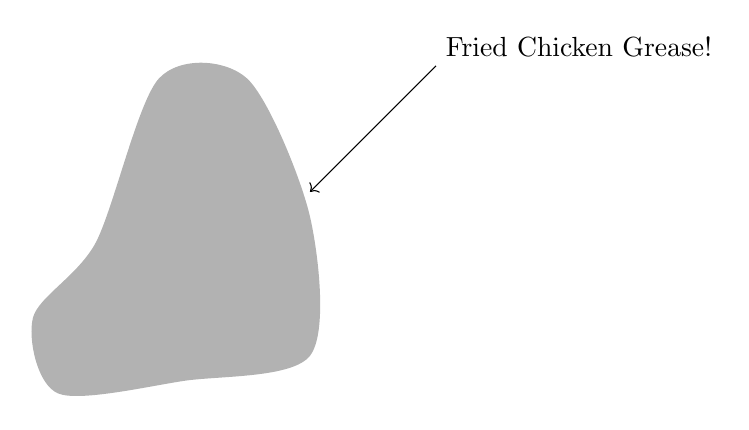
\begin{tikzpicture}[scale=1.6]
    \fill[black!30] plot [smooth cycle] coordinates {(0,0) (1,0.1) (2,0.3) (2,1.4) (1.5,2.5) (0.8,2.5) (0.3,1.2) (-0.2,0.6) };
    \draw[black, <-] (2,1.6) -- (3,2.6) node[black, anchor=south west] {Fried Chicken Grease!};
\end{tikzpicture}
\end{figure}

\vfill

\end{titlepage}

\newpage

\section*{Lecture 1: Introduction and Framing}
\setcounter{page}{1}

Electromagnetism is a field theory. As such, it requires us to specify two things:

\begin{enumerate}

\item[(1)] How matter produces fields

\item[(2)] How fields affect matter

\end{enumerate}

Note that for E\&M, ``matter'' means charges. \\

Point (1) is handled by the Maxwell equations. These are our source equations (\emph{i.e.} equations that describe how sources make fields).

\begin{table}[H]
\centering
\captionsetup{width=0.8\textwidth,labelfont={color=black,bf},textfont={color=black}}
\caption*{Maxwell's equations and their interpretation.}
\begin{tabular}{@{}c|c@{}}
\toprule
Equation & Interpretation \\ \midrule
{\parbox[c]{0.3\linewidth}{\begin{gather*} \nabla \cdot \bm{E} = \frac{\rho}{\epsilon_o} \end{gather*}}} & {\parbox[c]{0.6\linewidth}{\begin{center} $\bm{E}$-fields with divergence come from charges (electric monopoles). \end{center}}} \\ \midrule
{\parbox[c]{0.3\linewidth}{\begin{gather*} \nabla \cdot \bm{B} = 0 \end{gather*}}} & {\parbox[c]{0.6\linewidth}{\begin{center} $\bm{B}$-fields with divergence don't exist (no magnetic monopoles). \end{center}}} \\ \midrule
{\parbox[c]{0.3\linewidth}{\begin{gather*} \nabla \times \bm{E} = -\frac{\partial \bm{B}}{\partial t} \end{gather*}}} & {\parbox[c]{0.6\linewidth}{\begin{center} $\bm{E}$-fields with curl come from time-varying $\bm{B}$-fields --- and those \emph{only}. \end{center}}} \\ \midrule
{\parbox[c]{0.3\linewidth}{\begin{align*} \nabla \times \bm{B} &= \mu_o \bm{J} + \mu_o \epsilon_o \frac{\partial \bm{E}}{\partial t} \\ &= \mu_o \left( \bm{J} + \bm{J}_D \right) \end{align*}}} & {\parbox[c]{0.6\linewidth}{\begin{center} $\bm{B}$-fields with curl come from currents (moving electric monopoles) and from time-varying $\bm{E}$-fields. Sometimes we refer to $\epsilon_o \frac{\partial \bm{E}}{\partial t}$ as displacement current and bundle the $J$'s together. \end{center}}} \\ \bottomrule
\end{tabular}
\label{tab:1:maxwell}
\end{table}

Point (2) comes from the Lorentz force law: $\bm{F} = q \left( \bm{E} + \bm{v} \times \bm{B} \right)$. \\

Charges feel forces from $E$-fields \emph{always} and from $B$-fields when the charges are in motion. This means that observers in different inertial reference frames might disagree on whether a particular charge is experiencing a magnetic force at all, but that's okay.

Eventually we discover that fields themselves are different in different reference frames. This isn't a throwaway result since fields are very real things, carrying energy and momentum. \\

There's another equation that often gets listed as fundamental --- the so-called continuity equation:
\begin{equation*}
    \nabla \cdot \bm{J} = -\frac{\partial \rho}{\partial t}.
\end{equation*}

This is a statement of local conservation of charge: not only is charge conserved globally, in that the total amount never changes, but it's also conserved locally, meaning that to get from here to there, it has to move through the intervening space.

\begin{figure}[H]
\captionsetup{width=0.8\textwidth,labelfont={color=black,bf},textfont={color=black}}
\centering
\begin{subfigure}{0.55\linewidth}
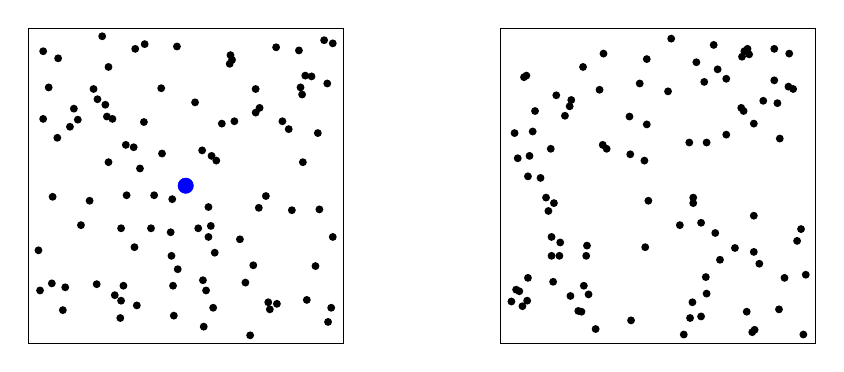
\begin{tikzpicture}
    \draw (0,0) -- (4,0) -- (4,4) -- (0,4) -- cycle;
    \foreach \x in {1,...,25}
        {
          \pgfmathrandominteger{\a}{10}{190}
          \pgfmathrandominteger{\b}{10}{190}
          \fill (\a*0.01,\b*0.01) circle (0.05);
        };
    \foreach \x in {1,...,25}
        {
          \pgfmathrandominteger{\a}{10}{190}
          \pgfmathrandominteger{\b}{210}{390}
          \fill (\a*0.01,\b*0.01) circle (0.05);
        };
    \foreach \x in {1,...,25}
        {
          \pgfmathrandominteger{\a}{210}{390}
          \pgfmathrandominteger{\b}{10}{190}
          \fill (\a*0.01,\b*0.01) circle (0.05);
        };
    \foreach \x in {1,...,25}
        {
          \pgfmathrandominteger{\a}{210}{390}
          \pgfmathrandominteger{\b}{210}{390}
          \fill (\a*0.01,\b*0.01) circle (0.05);
        };
    \fill[blue] (2,2) circle (0.1);
    \draw (6,0) -- (10,0) -- (10,4) -- (6,4) -- cycle;
    \foreach \x in {1,...,25}
        {
          \pgfmathrandominteger{\a}{610}{790}
          \pgfmathrandominteger{\b}{10}{190}
          \fill (\a*0.01,\b*0.01) circle (0.05);
        };
    \foreach \x in {1,...,25}
        {
          \pgfmathrandominteger{\a}{610}{790}
          \pgfmathrandominteger{\b}{210}{390}
          \fill (\a*0.01,\b*0.01) circle (0.05);
        };
    \foreach \x in {1,...,25}
        {
          \pgfmathrandominteger{\a}{810}{990}
          \pgfmathrandominteger{\b}{10}{190}
          \fill (\a*0.01,\b*0.01) circle (0.05);
        };
    \foreach \x in {1,...,25}
        {
          \pgfmathrandominteger{\a}{810}{990}
          \pgfmathrandominteger{\b}{210}{390}
          \fill (\a*0.01,\b*0.01) circle (0.05);
        };
        
    \fill[blue] (2,2) circle (0.1);
\end{tikzpicture}
\caption*{A \textcolor{blue}{blue dot} in the left box.}
\label{fig:1:continuitya} 
\end{subfigure}
~
\begin{subfigure}{0.55\linewidth}
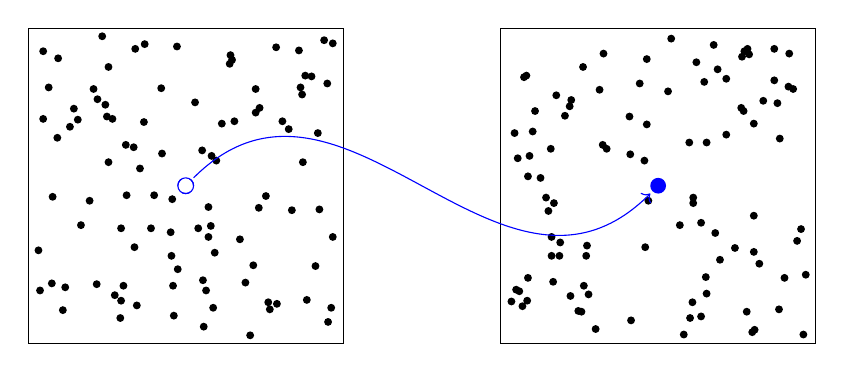
\begin{tikzpicture}
    \draw (0,0) -- (4,0) -- (4,4) -- (0,4) -- cycle;
    \foreach \x in {1,...,25}
        {
          \pgfmathrandominteger{\a}{10}{190}
          \pgfmathrandominteger{\b}{10}{190}
          \fill (\a*0.01,\b*0.01) circle (0.05);
        };
    \foreach \x in {1,...,25}
        {
          \pgfmathrandominteger{\a}{10}{190}
          \pgfmathrandominteger{\b}{210}{390}
          \fill (\a*0.01,\b*0.01) circle (0.05);
        };
    \foreach \x in {1,...,25}
        {
          \pgfmathrandominteger{\a}{210}{390}
          \pgfmathrandominteger{\b}{10}{190}
          \fill (\a*0.01,\b*0.01) circle (0.05);
        };
    \foreach \x in {1,...,25}
        {
          \pgfmathrandominteger{\a}{210}{390}
          \pgfmathrandominteger{\b}{210}{390}
          \fill (\a*0.01,\b*0.01) circle (0.05);
        };
    \draw[blue, dashed] (2,2) circle (0.1);
    \draw (6,0) -- (10,0) -- (10,4) -- (6,4) -- cycle;
    \foreach \x in {1,...,25}
        {
          \pgfmathrandominteger{\a}{610}{790}
          \pgfmathrandominteger{\b}{10}{190}
          \fill (\a*0.01,\b*0.01) circle (0.05);
        };
    \foreach \x in {1,...,25}
        {
          \pgfmathrandominteger{\a}{610}{790}
          \pgfmathrandominteger{\b}{210}{390}
          \fill (\a*0.01,\b*0.01) circle (0.05);
        };
    \foreach \x in {1,...,25}
        {
          \pgfmathrandominteger{\a}{810}{990}
          \pgfmathrandominteger{\b}{10}{190}
          \fill (\a*0.01,\b*0.01) circle (0.05);
        };
    \foreach \x in {1,...,25}
        {
          \pgfmathrandominteger{\a}{810}{990}
          \pgfmathrandominteger{\b}{210}{390}
          \fill (\a*0.01,\b*0.01) circle (0.05);
        };
        
    \draw[blue] (2,2) circle (0.1);
    \fill[blue] (8,2) circle (0.1);
    \draw[blue, ->] (2.1,2.1) .. controls (4,4) and (6,0) .. (7.9,1.9);
\end{tikzpicture}
\caption*{A \textcolor{blue}{blue dot} in the right box.}
\label{fig:1:continuityb}
\end{subfigure}
~
\caption*{An illustration of continuity. In order for the \textcolor{blue}{blue dot} to have move from the left box to the right box, it must necessarily have crossed through the intervening space.}
\label{fig:1:continuity}
\end{figure}

Conservation of charge is certainly fundamental, but it isn't a postulate - we can derive it from other laws. Start with the Ampere-Maxwell equation:
\begin{equation*}
    \nabla \times \bm{B} = \mu_o \bm{J} + \mu_o \epsilon_o \frac{\partial \bm{E}}{\partial t}.
\end{equation*}

Take the divergence of both sides:
\begin{gather*}
    \nabla \cdot \left( \nabla \times \bm{B} \right) = \nabla \cdot \left( \mu_o \bm{J} + \mu_o \epsilon_o \frac{\partial \bm{E}}{\partial t} \right) \\
    0 = \mu_o \left[ \nabla \cdot \bm{J} + \epsilon_o \nabla \cdot \left( \frac{\partial \bm{E}}{\partial t} \right) \right] \\
    0 = \nabla \cdot \bm{J} + \frac{d}{dt} \underbrace{\left( \epsilon_o \nabla \cdot \bm{E} \right)}_{\displaystyle = \rho} \\
    \implies \boxed{\nabla \cdot \bm{J} = -\frac{\partial \rho}{\partial t}}
\end{gather*}

For charge to be entering or leaving a region, there must be a divergence in the current. Note that this gives another way to tell that Amp{\'e}re's law ($\displaystyle \nabla \times \bm{B} = \mu_o \bm{J}$) is incomplete without Maxwell's correction. \\

\textbf{Interlude:} What are divergences and curls? \\

These Maxwell equations are in differential form, which is arguably the cleanest form, describing what's happening at a single point in space, as compared to the the integral forms that sample an entire region. We move back and forth between these forms using the divergence theorem and Stokes' theorem, which are higher dimensional generalizations of the fundamental theorem of calculus. \\

\textbf{Group activity:} convert Gauss's law from differential form to integral form and back using the divergence theorem. \\

Correct integral expressions aren't always super transparent. (Faraday clicker) 

For instance, $\displaystyle \oint \bm{E} \cdot d\bm{\ell} = -\frac{d}{dt} \int \bm{B} \cdot d\bm{A}$ with no qualifiers is simply false and will lead you to conclude that curly $\bm{E}$-fields exist when they don't. Consider the following.

$\displaystyle \oint \bm{E} \cdot d\bm{\ell} = -\int \frac{\partial \bm{B}}{\partial t} \cdot d\bm{A}$ is true always. And we can get the time-derivative out using the 3D Leibniz rule.
\begin{align*}
    \text{1D Leibniz Rule: }& \frac{d}{dt} \int_{a(t)}^{b(t)} f(x,t)\ dx = \frac{db}{dt} f(b,t) - \frac{da}{dt} f(a,t) + \int_a^b \frac{\partial}{\partial t} f(x, t)\ dx \\
    \text{3D Leibniz Rule: }& \frac{d}{dt} \int\limits_{A(t)} \bm{F}(\bm{x}, t) \cdot d\bm{A} = -\oint \left( \bm{v} \times \bm{F} \right) \cdot d\bm{\ell} + \int \left( \frac{\partial \bm{F}}{\partial t} + \left( \nabla \cdot \bm{F} \right) \bm{v} \right) \cdot d\bm{A}
\end{align*}

Letting $\bm{B}$ be the vector field gives
\begin{gather*}
    \frac{d}{dt} \int\limits_{A(t)} \bm{B}(\bm{x}, t) \cdot d\bm{A} = \int \left( \frac{\partial \bm{B}}{\partial t} + \cancelto{0}{\left( \nabla \cdot \bm{B} \right)} \bm{v} \right) \cdot d\bm{A} - \oint \left( \bm{v} \times \bm{B} \right) \cdot d\bm{\ell} \\
    \implies \frac{d}{dt} \int \bm{B} \left( \bm{x}, t \right) \cdot d\bm{A} + \oint \left( \bm{v} \times \bm{B} \right) \cdot d\bm{\ell} = \int \frac{\partial \bm{B}}{\partial t} \cdot d\bm{A}
\end{gather*}

Again, we know that $\displaystyle \oint \bm{E} \cdot d\bm{\ell} = -\int \frac{\partial \bm{B}}{\partial t} \cdot d\bm{A}$ is true always. So sub into that we get
\begin{gather*}
    \oint \bm{E} \cdot d\bm{\ell} = -\frac{d}{dt} \int \bm{B} \cdot d\bm{A} - \oint \left( \bm{v} \times \bm{B} \right) \cdot d\bm{\ell} \\
    \implies \underbrace{\oint \left( \bm{E} + \bm{v} \times \bm{B} \right) \cdot d\bm{\ell}}_{\displaystyle \text{emf}} \quad = \quad \underbrace{-\frac{d}{dt} \int \bm{B} \cdot d\bm{A}}_{\displaystyle -\frac{d\Phi}{dt}}
\end{gather*}

Which is the correct integral form of Faraday's law, and explicitly shows both the $\bm{E}$-field and the motional contributions to the emf.

Altogether, Maxwell's equations
\begin{gather*}
    \nabla \cdot \bm{E} = \frac{\rho}{\epsilon_o} \qquad\qquad \nabla \cdot \bm{B} = 0 \\
    \nabla \times \bm{E} = -\frac{\partial \bm{B}}{\partial t} \qquad\qquad \nabla \times \bm{B} = \mu_o \bm{J} + \mu_o\epsilon_o \frac{\partial \bm{E}}{\partial t}
\end{gather*}

and the Lorentz force law
\begin{equation*}
    \bm{F} = q\left( \bm{E} + \bm{v} \times \bm{B} \right)
\end{equation*}

give us all of classical E\&M. The rest is sorting out the details.

\newpage

\section*{Lecture 2: Coulomb's and Gauss's Laws}
\setcounter{page}{1}

The general set of equations governing electromagnetism is as follows:
\begin{gather*}
    \text{Maxwell's equations}\begin{cases} \displaystyle \nabla \cdot \bm{E} = \frac{\rho}{\epsilon_o} \\[0.4cm] \displaystyle \nabla \cdot \bm{B} = 0 \\[0.4cm] \displaystyle \nabla \times \bm{E} = -\frac{\partial \bm{B}}{\partial t} \\[0.4cm] \displaystyle \nabla \times \bm{B} = \mu_o \bm{J} + \mu_o\epsilon_o \frac{\partial \bm{E}}{\partial t} \end{cases} \qquad\qquad \underbrace{\bm{F} = q \left( \bm{E} + \bm{v} \times \bm{B} \right)}_{\displaystyle \text{Lorentz force law}}
\end{gather*}

But we don't generally try to tackle that all at once. We'll get started by studying what happens when all the charges in the neighborhood are fixed in place --- what we call \underline{electrostatics}. Then, all the time-varying terms go away, as do the currents, and in fact \underline{all} sources of $\bm{B}$-fields, leaving us with just
\begin{gather*}
    \begin{cases} \displaystyle \nabla \cdot \bm{E} = \frac{\rho}{\epsilon_o} \\[0.4cm] \displaystyle \nabla \times \bm{E} = \bm{0} \end{cases} \qquad\qquad \bm{F} = q\bm{E}
\end{gather*}

And as an added bonus, you can even derive $\displaystyle \nabla \times \bm{E} = \bm{0}$ for Gauss's law, leaving us with only two unique equations. We might look at that derivation later on if we have time.

Now, you may not be accustomed to seeing Gauss's law in differential form, so let's convert it to integral form. Integrating over some volume:
\begin{equation*}
    \int \left( \nabla \cdot \bm{E} \right) d^3x' = \int \frac{\rho}{\epsilon_o}\ d^3x' \qquad\qquad \parbox[c]{0.5\textwidth}{Note that there are several conventions for writing a differential volume element. Using $dV$ is not preferred, since we sometimes use it for a differential voltage. You'll see $d^3x$, $dv$, and even $d\tau$.}
\end{equation*}

On the right, integrating a volume charge density over a volume gives a charge:
\begin{equation*}
    \int \frac{\rho}{\epsilon_o}\ d^3x' \quad = \quad \frac{1}{\epsilon_o} \underbrace{\int \rho\ d^3x'}_{\displaystyle \text{charge}} \quad = \quad \frac{Q_{\text{encl}}}{\epsilon_o}.
\end{equation*}

On the left, we can apply the divergence theorem:
\begin{equation*}
    \int \left( \nabla \cdot \bm{E} \right)\ d^3x' = \oint \bm{E} \cdot d\bm{A}.
\end{equation*}

Putting the two together, we obtain the familiar intro version of Gauss's law:
\begin{equation*}
    \boxed{\oint \bm{E} \cdot d\bm{A} = \frac{Q_{\text{enc}}}{\epsilon_o}} \qquad\qquad \parbox[c]{0.5\textwidth}{You can take the integral form and derive it from the differential form. The steps are \underline{almost} identical but in reverse, except for one tricky part that I won't spoil for you.}
\end{equation*}

These forms are equivalent insofar as you can derive one from the other, but say slightly different things. The differential form is a statement about \underline{single points} in space --- if there's some non-zero $\rho$ at a point, there's also a diverging $\bm{E}$-field there. The integral form is a statement about whole regions --- the flux through some shape is proportional to the amount of charge it encloses.

I promised that you can get all of electrostatics from $\displaystyle \nabla \cdot \bm{E} = \frac{\rho}{\epsilon_o}$ and $\bm{F} = q\bm{E}$, and you can. That includes Coulomb's law, as long as we include one more not-terribly-controversial postulate. Start with a positive point charge of magnitude $q$ at the origin:

\begin{minipage}{0.5\textwidth}
\begin{flushleft}
\begin{figure}[H]
\captionsetup{width=0.8\textwidth,labelfont={color=black,bf},textfont={color=black}}
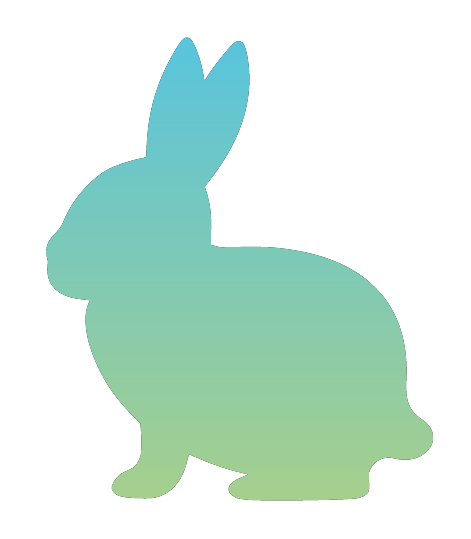
\begin{tikzpicture}
    \node at (0,0) {\bunny[scale=2.5, top color=BLUE_C, bottom color=GREEN_B]};
\end{tikzpicture}
\label{fig:2:point}
\end{figure}
\end{flushleft}
\end{minipage}
~
\begin{minipage}{0.5\textwidth}
\begin{flushright}
\parbox[c]{\textwidth}{If we posit that space is rotationally invariant (changing the orientation of a system doesn't change the physics), we can immediately conclude that a point charge (being spherically symmetric) must produce a strictly radial field. To see this, try a little proof by contradiction.}
\end{flushright}
\end{minipage}

\begin{minipage}{0.5\textwidth}
\begin{flushleft}
\begin{figure}[H]
\captionsetup{width=0.8\textwidth,labelfont={color=black,bf},textfont={color=black}}
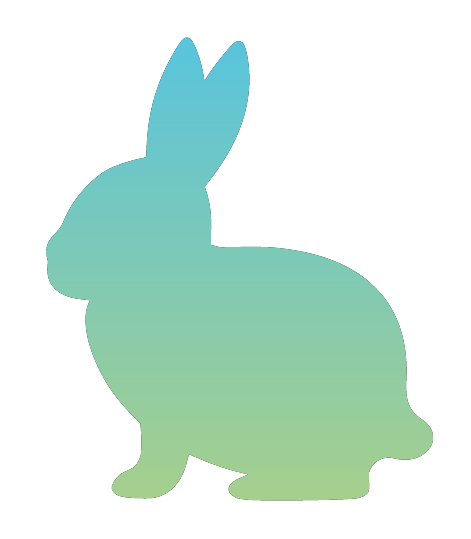
\begin{tikzpicture}
    \node at (0,0) {\bunny[scale=2.5, top color=BLUE_C, bottom color=GREEN_B]};
\end{tikzpicture}
\label{fig:2:b}
\end{figure}
\end{flushleft}
\end{minipage}
~
\begin{minipage}{0.5\textwidth}
\begin{flushright}
\parbox[c]{\textwidth}{Suppose the charge makes some non-radial field at some point. Then suppose suppose we take the whole system and rotate it \ang{180} about the indicated axis.}
\end{flushright}
\end{minipage}

\begin{minipage}{0.5\textwidth}
\begin{flushleft}
\begin{figure}[H]
\captionsetup{width=0.8\textwidth,labelfont={color=black,bf},textfont={color=black}}
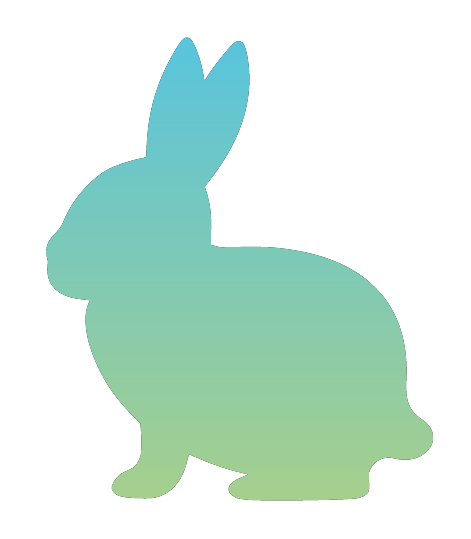
\begin{tikzpicture}
    \node at (0,0) {\bunny[scale=2.5, top color=BLUE_C, bottom color=GREEN_B]};
\end{tikzpicture}
\label{fig:2:c}
\end{figure}
\end{flushleft}
\end{minipage}
~
\begin{minipage}{0.5\textwidth}
\begin{flushright}
\parbox[c]{\textwidth}{The actual charge is unchanged, but now it makes the opposite field! This is kind of nonsense, and our claim that there could be a non-radial field must have been false.}
\end{flushright}
\end{minipage}

\begin{minipage}{0.5\textwidth}
\begin{flushleft}
\begin{figure}[H]
\captionsetup{width=0.8\textwidth,labelfont={color=black,bf},textfont={color=black}}
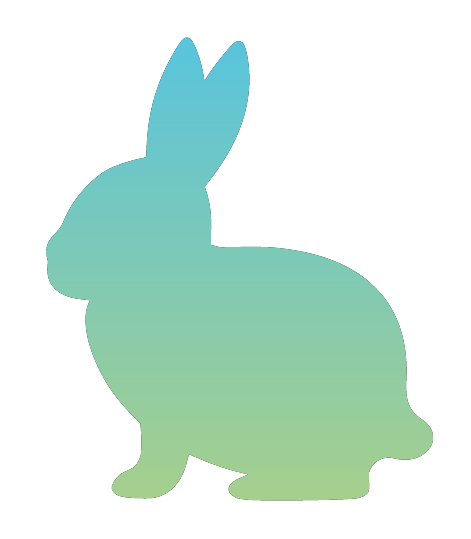
\begin{tikzpicture}
    \node at (0,0) {\bunny[scale=2.5, top color=BLUE_C, bottom color=GREEN_B]};
\end{tikzpicture}
\label{fig:2:d}
\end{figure}
\end{flushleft}
\end{minipage}
~
\begin{minipage}{0.5\textwidth}
\begin{flushright}
\parbox[c]{\textwidth}{So we have a radial field. Let's draw a spherical Gaussian surface of radius $r$ around the point charge, and write down Gauss's law.}
\end{flushright}
\end{minipage}

\begin{minipage}{0.5\textwidth}
\begin{flushleft}
\begin{equation*}
    \oint \bm{E} \cdot d\bm{A} = \frac{Q_{\text{enc}}}{\epsilon_o}
\end{equation*}
\end{flushleft}
\end{minipage}
~
\begin{minipage}{0.5\textwidth}
\begin{flushright}
\parbox[c]{\textwidth}{We're integrating $\bm{E} \cdot d\bm{A}$ all around the Gaussian sphere. The differential area vector $d\bm{A}$ corresponds to a little patch of that surface, and points radially outward. The electric field $\bm{E}$ also points radially outward everywhere, so at any point on the Gaussian surface $\bm{E} \cdot d\bm{A} = E\ dA$. (And $Q_{\text{enc}} = q$, naturally.)}
\end{flushright}
\end{minipage}

\vspace{1cm}

\begin{minipage}{0.36\textwidth}
\begin{flushleft}
\begin{equation*}
    \implies \oint E\ dA = \frac{q}{\epsilon_o}
\end{equation*}
\end{flushleft}
\end{minipage}
~
\begin{minipage}{0.64\textwidth}
\begin{flushright}
\parbox[c]{\textwidth}{Now, this system is rotationally invariant (it has spherical symmetry), so the magnitude of $\bm{E}$ has to be the same everywhere on the domain of integration, and we can pull it out.}
\end{flushright}
\end{minipage}

\begin{gather*}
    \implies E \oint dA = \frac{q}{\epsilon_o} \qquad\qquad \parbox[c]{0.5\textwidth}{$\displaystyle \oint dA$ is just the area of the Gaussian surface, or $\displaystyle 4\pi r^2$ in this case.} \\
    \implies E \left( 4\pi r^2 \right) = \frac{q}{\epsilon_o} \qquad\qquad \parbox[c]{0.5\textwidth}{\textcolor{white}{here}} \\
    \implies E = \frac{q}{4\pi \epsilon_o\ r^2} \qquad\qquad \parbox[c]{0.5\textwidth}{And we know the the electric field is radial, so}
\end{gather*}

\begin{equation*}
    \boxed{\bm{E}_{\text{point}} = \frac{q}{4\pi\epsilon_o\ r^2} \rhat = \frac{q}{4\pi\epsilon_o} \frac{\bm{r}}{r^3}} \qquad\qquad \parbox[c]{0.2\textwidth}{Which is indeed Coulomb's law}
\end{equation*}

\subsection*{Coulomb's \& Gauss's Laws}

Coulomb's Law is derived empirically and reads
\begin{equation*}
    \bm{F} = \frac{k q_1 q_2\ \rhat}{r^2} = \frac{k q_1 q_2\ \bm{r}}{r^3} \qquad \text{or} \qquad \bm{F} = \frac{k q_1 q_2\ \left( \bm{x} - \bm{x'} \right)}{\left| \bm{x} - \bm{x'} \right|^3}
\end{equation*}

We define the electric field via
\begin{equation*}
    \begin{rcases} \displaystyle \bm{E} = \frac{\bm{F}}{q} \implies \bm{E} = \frac{kq\ \rhat}{r^2} \\ \displaystyle \qquad\qquad\Updownarrow \\ \displaystyle \bm{E} = \frac{1}{4\pi\epsilon_o} \frac{q\ \left( \bm{x} - \bm{x'} \right)}{\left| \bm{x} - \bm{x'} \right|^3} \end{rcases} \text{Often still called Coulomb's law. Note that } k = \frac{1}{4\pi\epsilon_o}
\end{equation*}

Superposition applies. That is, the net electric field at a point is the sum of the contributions from the (discrete) constituent charges:
\begin{equation*}
    \bm{E}_{\text{net}} = \sum\limits_{i = 1}^N \frac{k q_i\ \rhat}{r^2} \qquad \text{or} \qquad \bm{E}(\bm{x}) = \frac{1}{4\pi\epsilon_o} \sum\limits_{i = 1}^{N} \frac{q_i\ \left( \bm{x} - \bm{x'} \right)}{\left| \bm{x} - \bm{x'} \right|^3}
\end{equation*}

This can be generalized to continuous distributions by considering a differential amount of charge $dq$:
\begin{equation*}
    d\bm{E} = \frac{k\ dq\ \bm{r}}{r^3} \qquad \text{or} \qquad d\bm{E} = \frac{1}{4\pi\epsilon_o} \frac{dq\ \left( \bm{x} - \bm{x'} \right)}{\left| \bm{x} - \bm{x'} \right|^3}
\end{equation*}

\begin{mdframed}[backgroundcolor=WHITE,align=left,userdefinedwidth=45em, topline=false, rightline=false,frametitle={Warning on Notation}]

We frequently encounter problems involving two points:
\begin{itemize}

\item Source points, $\bm{x'}$, which are denoted with primed coordinates. These represent the locations of whatever is producing the field (\emph{i.e.} the location of charges).

\item Field points, $\bm{x}$, which are denoted with unprimed coordinates. These represent the location of interest (\emph{i.e.} the point at which the electric field is being calculated).

\end{itemize}

Sometimes, a short-hand notation is adopted in which these vectors are combined into one \emph{separation vector} $\bm{r}$:
\begin{equation*}
    \bm{r} \equiv \bm{x} - \bm{x'}. \qquad\qquad \parbox[c]{0.5\textwidth}{Note that Griffiths denotes the separation vector with a script $\scripty{r}$.}
\end{equation*}

Its magnitude is
\begin{equation*}
    r = \left| \bm{x} - \bm{x'} \right|,
\end{equation*}

and a unit vector in the direction from $\bm{x'}$ to $\bm{x}$ is
\begin{equation*}
    \rhat = \frac{\bm{r}}{r} = \frac{\bm{x} - \bm{x'}}{\left| \bm{x} - \bm{x'} \right|}.
\end{equation*}

For consistency, we will usually keep source and field vectors separate.

\end{mdframed}

Suppose the source of the electric field is instead distributed continuously over some region. Then the sum becomes an integral:
\begin{equation*}
    \bm{E}(\bm{x}) = \frac{1}{4\pi\epsilon_o} \int \frac{dq\ \left( \bm{x} - \bm{x'} \right)}{\left| \bm{x} - \bm{x'} \right|^3}.
\end{equation*}

What we use for $dq$ amounts to what dimension the charge is distributed over.

\begin{table}[H]
\centering
\captionsetup{width=0.8\textwidth,labelfont={color=black,bf},textfont={color=black}}
\begin{tabular}{@{}c|c|c@{}}
\toprule
Continuous charge distribution & Differential charge & Electric field expression \\ \midrule
Line charge, $\lambda$ & \parbox[c]{0.2\textwidth}{\begin{align*} dq &= \lambda\ dx' \\ &= \lambda\ dl' \end{align*}} & \parbox[c]{0.4\textwidth}{\begin{equation*} \bm{E}(\bm{x}) = \frac{1}{4\pi\epsilon_o} \int \frac{\lambda(\bm{x'})\ dx'\ \ \left( \bm{x} - \bm{x'} \right)}{\left| \bm{x} - \bm{x'} \right|^3} \end{equation*}} \\ \midrule
Surface charge, $\sigma$ & \parbox[c]{0.2\textwidth}{\begin{align*} dq &= \sigma\ d^2x' \\ &= \sigma\ dA' \end{align*}} & \parbox[c]{0.4\textwidth}{\begin{equation*} \bm{E}(\bm{x}) = \frac{1}{4\pi\epsilon_o} \int \frac{\sigma(\bm{x'})\ d^2x'\ \ \left( \bm{x} - \bm{x'} \right)}{\left| \bm{x} - \bm{x'} \right|^3} \end{equation*}} \\ \midrule
Volume charge, $\rho$ & \parbox[c]{0.2\textwidth}{\begin{align*} dq &= \rho\ d^3x' \\ &= \rho\ d\tau' \end{align*}} & \parbox[c]{0.4\textwidth}{\begin{equation*} \bm{E}(\bm{x}) = \frac{1}{4\pi\epsilon_o} \int \frac{\rho(\bm{x'})\ d^3x'\ \ \left( \bm{x} - \bm{x'} \right)}{\left| \bm{x} - \bm{x'} \right|^3} \end{equation*}} \\ \bottomrule
\end{tabular}
\label{tab:2:dq}
\end{table}


Coulomb's law + superposition + some math generates \underline{all} of electrostatics. \\

(Clicker question) \\

Let's do a nice Coulomb's law derivation. We have seen via Gauss's law that spherically symmetric charge distributions behave identically to point charges viewed from the outside. Moreover, symmetric shells have zero electric field inside. We'll show this via integration.

First, we choose to believe that the spherical symmetry gives us a strictly radial field (more on this later) and as a fun trick, we look at the field at some distance along the $z$-axis.

\begin{minipage}{0.4\textwidth}
\begin{flushleft}
\begin{figure}[H]
\captionsetup{width=0.8\textwidth,labelfont={color=black,bf},textfont={color=black}}
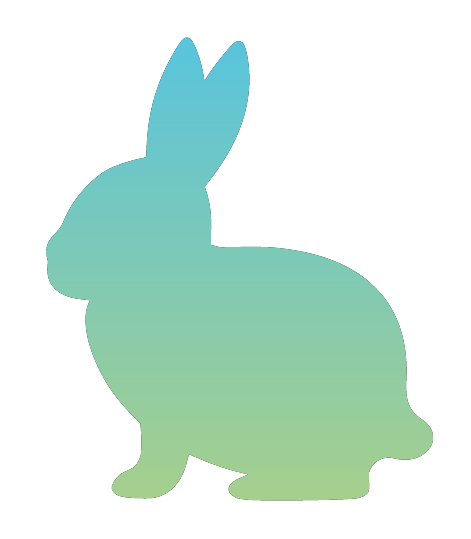
\begin{tikzpicture}
    \node at (0,0) {\bunny[scale=2.5, top color=BLUE_C, bottom color=GREEN_B]};
\end{tikzpicture}
\label{fig:2:e}
\end{figure}
\end{flushleft}
\end{minipage}
~
\begin{minipage}{0.6\textwidth}
\begin{flushright}
\parbox[l]{\textwidth}{Start with the general expression for the electric field made by a surface charge:}
\begin{gather*}
    \bm{E}(\bm{x}) = \frac{1}{4\pi\epsilon_o} \int \frac{dq\ \left( \bm{x} - \bm{x'} \right)}{\left| \bm{x} - \bm{x'} \right|^3} = \frac{1}{4\pi\epsilon_o} \int \frac{\sigma\ dA'\ \ \left( \bm{x} - \bm{x'} \right)}{\left| \bm{x} - \bm{x'} \right|^3} \\[0.3cm]
    dq = \sigma\ dA' = \sigma\ R^2 \sin{\theta'}\ d\theta'\ d\phi'
\end{gather*}

\parbox[l]{\textwidth}{Consider the source and field position vectors:}
\begin{equation*}
    \begin{cases} \displaystyle \bm{x} = z\ \khat \\ \displaystyle \bm{x'} = R\ \rhat = R\sin{\theta'}\cos{\phi'}\ \ihat + R\sin{\theta'}\sin{\phi'}\ \jhat + R\cos{\theta'}\ \khat \end{cases}
\end{equation*}

\parbox[l]{\textwidth}{Forming their difference gives}
\begin{equation*}
    \bm{x} - \bm{x'} = \left( -R\sin{\theta'}\cos{\phi'} \right) \ihat + \left( -R\sin{\theta'}\sin{\phi'} \right) \jhat + \left( z - R\cos{\theta'} \right) \khat
\end{equation*}
\end{flushright}
\end{minipage}

The magnitude of the separation vector is
\begin{align*}
    \left| \bm{x} - \bm{x'} \right| &= \sqrt{\left( -R\sin{\theta'}\cos{\phi'} \right)^2 + \left( -R\sin{\theta'}\sin{\phi'} \right)^2 + \left( z - R\cos{\theta'} \right)^2} \\
    %&= \sqrt{R^2 \sin^2{\theta'}\cos^2{\phi'} + R^2 \sin^2{\theta'}\sin^2{\phi'} + \left( z - R\cos{\theta'} \right)^2} \\
    &= \sqrt{R^2 \sin^2{\theta'} \left( \cos^2{\phi'} + \sin^2{\phi'} \right) + \left( z - R\cos{\theta} \right)^2} \\
    &= \sqrt{R^2 \sin^2{\theta'} + z^2 - 2Rz\cos{\theta'} + R^2 \cos^2{\theta'}} \\
    %&= \sqrt{R^2 \left( \cos^2{\theta'} + \sin^2{\theta'} \right) + z^2 - 2Rz \cos{\theta'}} \\
    &= \sqrt{R^2 + z^2 - 2Rz\cos{\theta'}}
\end{align*}

Putting it all together,
\begin{align*}
    \bm{E}(\bm{x}) &= \frac{1}{4\pi\epsilon_o} \int \frac{\sigma dA'\ \left( \bm{x} - \bm{x'} \right)}{\left| \bm{x} - \bm{x'} \right|^3} \\
    &= \frac{1}{4\pi\epsilon_o} \left( \cancelto{0}{\int \frac{\sigma\ dA'\ \left( -R\sin{\theta'}\cos{\phi'} \right) \ihat}{\left| \bm{x} - \bm{x'} \right|^3}} + \cancelto{0}{\int \frac{\sigma\ dA'\ \left( -R\sin{\theta'}\sin{\phi'} \right) \jhat}{\left| \bm{x} - \bm{x'} \right|^3}} + \int \frac{\sigma\ dA'\ \left( z - R\cos{\theta'} \right) \khat}{\left| \bm{x} - \bm{x'} \right|^3} \right) \\
    &= \frac{1}{4\pi\epsilon_o} \int_0^{2\pi} \int_{0}^{\pi} \frac{\sigma\ R^2 \sin{\theta'}\ d\theta'\ d\phi'\ \ \left( z - R\cos{\theta'} \right)}{\left( R^2 + z^2 - 2Rz \cos{\theta'} \right)^{3/2}}\ \khat.
\end{align*}

The terms corresponding to the $\ihat$ and $\jhat$ components of the separation vector $\bm{x} - \bm{x'}$ vanish (note we are integrating $\cos{\phi'}$ and $\sin{\phi'}$, respectively, from $0$ to $2\pi$ --- physically this corresponds to the symmetry about the $z$-axis). This leaves us with
\begin{align*}
    \bm{E} &= \frac{1}{4\pi\epsilon_o} \int_0^{2\pi} \int_{0}^{\pi} \frac{\sigma\ R^2 \sin{\theta'}\ d\theta'\ d\phi'\ \ \left( z - R\cos{\theta'} \right)}{\left( R^2 + z^2 - 2Rz \cos{\theta'} \right)^{3/2}}\ \khat \\
    &= \frac{\sigma\ R^2}{2\epsilon_o} \int_{0}^{\pi} \frac{\sin{\theta'}\ d\theta'\ \left( z - R \cos{\theta'} \right)}{\left( R^2 + z^2 - 2Rz\cos{\theta'} \right)^{3/2}}
\end{align*}

Substituting $u = \cos{\theta'}$ and $du = -\sin{\theta'}\ d\theta'$,
\begin{align*}
    \bm{E} &= \frac{\sigma R^2}{2\epsilon_o} \int_{-1}^{1} \frac{-du\ \left( z - Ru \right)}{\left( R^2 + z^2 - 2Rzu \right)^{3/2}}\ \khat
\end{align*}

Using integration tables or software,
\begin{align*}
    \bm{E} &= \frac{\sigma R^2}{2\epsilon_o} \Eval{\left( \frac{zu - R}{z^2 \sqrt{R^2 + z^2 - 2Rzu}} \right)}{-1}{1}\ \khat \\
    &= \frac{\sigma R^2}{2\epsilon_o\ z^2} \left[ \left( \frac{z - R}{\sqrt{R^2 + z^2 - 2Rz}} \right) + \cancelto{1}{\left( \frac{z + R}{\sqrt{R^2 + z^2 + 2Rz}} \right)} \right]\ \khat \\
    &= \frac{\sigma R^2}{2\epsilon_o\ z^2} \left[ \frac{z - R}{\sqrt{\left( z - R \right)^2}} + 1 \right]\ \khat \\
    &= \frac{\sigma R^2}{2\epsilon_o\ z^2} \left[ \frac{z - r}{\left| z - R \right|} + 1 \right]\ \khat.
\end{align*}

If $z < R$ (inside the sphere), then $\displaystyle \frac{z - r}{\left| z - R \right|} = -1$ and we get
\begin{equation*}
    \bm{E}_{\text{inside}} = \frac{\sigma R^2}{2\epsilon_o\ z^2} \left[ -1 + 1 \right]\ \khat = \bm{0}.
\end{equation*}

If $z > R$ (outside the sphere), then $\displaystyle \frac{z - r}{\left| z - R \right|} = 1$ and we get
\begin{equation*}
    \bm{E}_{\text{outside}} = \frac{\sigma R^2}{2\epsilon_o\ z^2} \left[ 1 + 1 \right]\ \khat = \frac{\sigma\ R^2}{\epsilon_o\ z^2}\ \khat.
\end{equation*}

Since the charge is uniformly distributed, $\displaystyle \sigma = \frac{Q}{4\pi R^2}$. With this substitution, the electric field outside becomes
\begin{equation*}
    \bm{E}_{\text{outside}} = \frac{Q}{4\pi\ R^2} \frac{R^2}{\epsilon_o\ z^2}\ \khat = \frac{Q}{4\pi\epsilon_o\ z^2}\ \khat.
\end{equation*}

We've gotten this result before with Gauss's law, and as it turns out Coulomb's law implies Gauss's law, and vice-versa (almost). Deriving Gauss's law from Coulomb's law is hard to do formally, so let's skip the derivation for now. Instead, recall the definition of flux:
\begin{equation*}
    \Phi \equiv \int \bm{E} \cdot d\bm{A}.
\end{equation*}

Gauss's law is a statement about the flux through a closed surface, and is \underline{always} true. If we have good symmetry (maybe planar, cylindrical, or spherical in nature), we will \underline{also} be able to solve for $\bm{E}$. But we make many remarkably subtle arguments along the way. \\

Let's consider an infinite homogeneous sheet of charge, in Cartesian coordinates, with charge density $\sigma$.

\begin{minipage}{0.4\textwidth}
\begin{flushleft}
\begin{figure}[H]
\captionsetup{width=0.8\textwidth,labelfont={color=black,bf},textfont={color=black}}
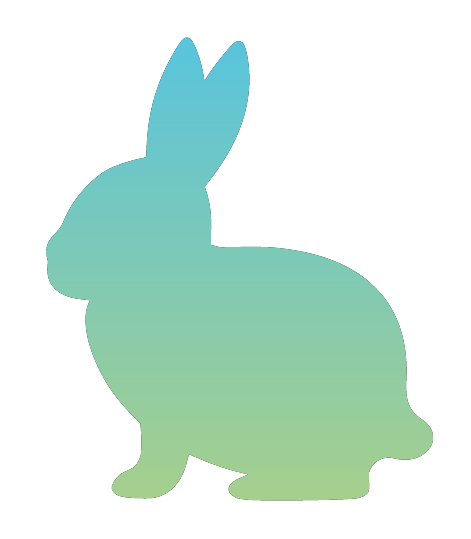
\begin{tikzpicture}
    \node at (0,0) {\bunny[scale=2.5, top color=BLUE_C, bottom color=GREEN_B]};
\end{tikzpicture}
\label{fig:2:g}
\end{figure}
\end{flushleft}
\end{minipage}
~
\begin{minipage}{0.6\textwidth}
\begin{flushright}
\parbox[c]{\textwidth}{Suppose there exists a component of $\bm{E}$ in the $\ihat$-direction. Now, the sheet has a variety of symmetries, including symmetry under reflection and rotation. Twisting the sheet about the $z$-axis doesn't change it and thus can't change the field. So assuming $E_x$ is non-zero leads to a contradiction. Similarly, there can't be a component of the field in the $\jhat$-direction. To wit: $E_x = E_y = 0$.}
\end{flushright}
\end{minipage}

The $\khat$-component of the electric field, $E_z$, respects all available symmetries and so can exist. Assuming a positively charged sheet, the electric field points away from the sheet. I therefore draw a Gaussian surface like so.

\begin{minipage}{0.4\textwidth}
\begin{flushleft}
\begin{figure}[H]
\captionsetup{width=0.8\textwidth,labelfont={color=black,bf},textfont={color=black}}
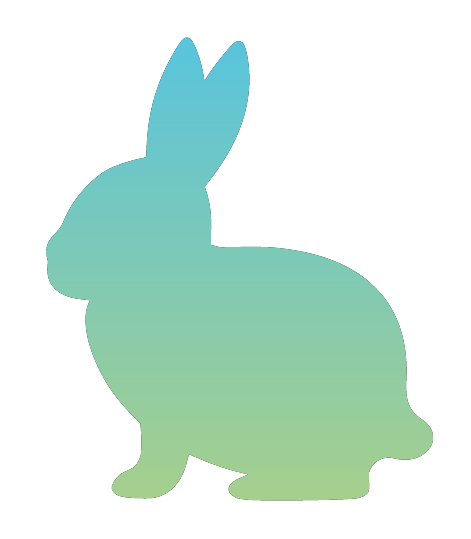
\begin{tikzpicture}
    \node at (0,0) {\bunny[scale=2.5, top color=BLUE_C, bottom color=GREEN_B]};
\end{tikzpicture}
\label{fig:2:g}
\end{figure}
\end{flushleft}
\end{minipage}
~
\begin{minipage}{0.6\textwidth}
\begin{flushright}
\begin{equation*}
    \oint \bm{E} \cdot d\bm{A} = \frac{Q_{\text{enc}}}{\epsilon_o} \qquad\qquad \parbox[c]{0.5\textwidth}{We will work the left-hand side of Gauss's law first.}
\end{equation*}
\parbox[c]{\textwidth}{\begin{equation*} \oint \bm{E} \cdot d\bm{A} = \hspace{-0.2cm} \int\limits_{\parbox[c]{0.1\textwidth}{\begin{center} \tiny top + \\ bottom \end{center}}} \hspace{-0.4cm} \bm{E} \cdot d\bm{A} = \hspace{-0.2cm} \int\limits_{\parbox[c]{0.1\textwidth}{\begin{center} \tiny top + \\ bottom \end{center}}} \hspace{-0.4cm} E\ dA = E \hspace{-0.2cm} \int\limits_{\parbox[c]{0.1\textwidth}{\begin{center} \tiny top + \\ bottom \end{center}}} \hspace{-0.4cm} dA = E \left( 2 A_{\text{top}} \right) \end{equation*}}
\parbox[c]{\textwidth}{\underline{Every single step} came with a reason. Know them.}
\end{flushright}
\end{minipage}

Now, $\displaystyle Q_{\text{enc}} = \sigma A_{\text{top}}$, so
\begin{equation*}
    \oint \bm{E} \cdot d\bm{A} = \frac{Q_{\text{enc}}}{\epsilon_o} \quad \implies \quad E \left( 2 A_{\text{top}} \right) = \frac{\sigma A_{\text{top}}}{\epsilon_o} \quad \implies \quad \boxed{E_{\text{sheet}} = \frac{\sigma}{2\epsilon_o}}
\end{equation*}

\begin{minipage}{0.4\textwidth}
\begin{flushleft}
\begin{figure}[H]
\captionsetup{width=0.8\textwidth,labelfont={color=black,bf},textfont={color=black}}
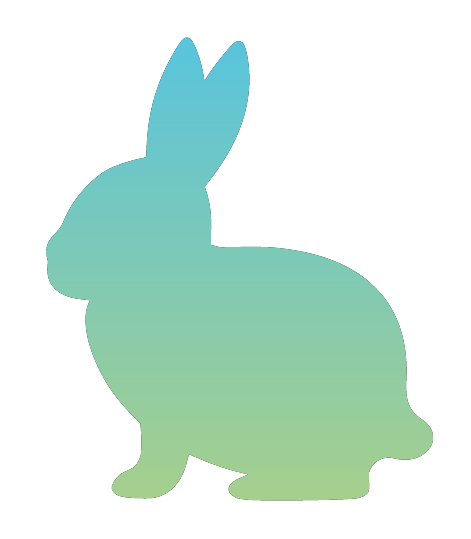
\begin{tikzpicture}
    \node at (0,0) {\bunny[scale=2.5, top color=BLUE_C, bottom color=GREEN_B]};
\end{tikzpicture}
\label{fig:2:h}
\end{figure}
\end{flushleft}
\end{minipage}
~
\begin{minipage}{0.6\textwidth}
\begin{flushright}
\parbox[c]{\textwidth}{\begin{flushleft} Notice the discontinuity in the perpendicular component of the $\bm{E}$-field (denoted $E^{\perp}$): \end{flushleft}}
\parbox[c]{\textwidth}{\begin{equation*} \boxed{E_{\text{above}}^{\perp} - E_{\text{below}}^{\perp} = \frac{\sigma}{\epsilon_o}} \end{equation*}}
\parbox[c]{\textwidth}{\begin{flushleft} This is always true. We can always zoom in until the surface is locally flat and draw a Gaussian box. \end{flushleft}}
\end{flushright}
\end{minipage}

This is a boundary condition. It will come back, and it will bring a friend.

\begin{minipage}{0.4\textwidth}
\begin{flushleft}
\begin{figure}[H]
\captionsetup{width=0.8\textwidth,labelfont={color=black,bf},textfont={color=black}}
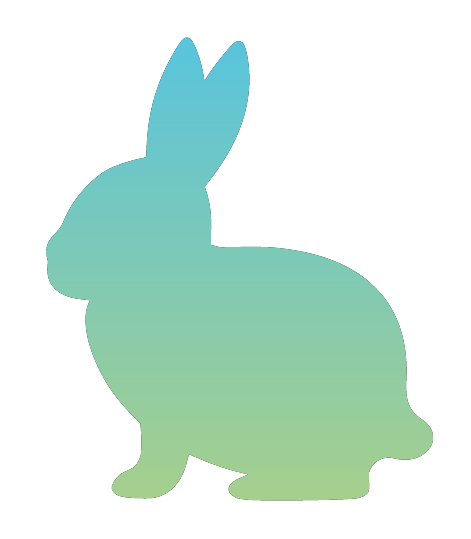
\begin{tikzpicture}
    \node at (0,0) {\bunny[scale=2.5, top color=BLUE_C, bottom color=GREEN_B]};
\end{tikzpicture}
\label{fig:2:i}
\end{figure}
\end{flushleft}
\end{minipage}
~
\begin{minipage}{0.6\textwidth}
\begin{flushright}
\parbox[c]{\textwidth}{\begin{flushleft} Consider the component of the $\bm{E}$-field parallel to the surface, $E^{\parallel}$. Assume $\nabla \times \bm{E} = \bm{0}$. \end{flushleft}}
\textcolor{white}{here}
\parbox[c]{\textwidth}{Then, applying Stokes' theorem to the loop shown, }
\parbox[c]{\textwidth}{\begin{equation*} \oint \bm{E} \cdot d\bm{\ell} = \int \left( \nabla \times \bm{E} \right) \cdot d\bm{A} = 0 \end{equation*}}
\parbox[c]{\textwidth}{As the loop gets small, we must have}
\parbox[c]{\textwidth}{\begin{equation*} \boxed{E_{\text{above}}^{\parallel} = E_{\text{below}}^{\parallel}} \end{equation*}}
\parbox[c]{\textwidth}{\begin{flushleft} That is, $E^{\parallel}$ is always continous across surfaces. \end{flushleft}}
\end{flushright}
\end{minipage}

Now, how is it that $\displaystyle \nabla \times \bm{E} = \bm{0}$? This is easy to show with Faraday's law, which reads
\begin{equation*}
    \nabla \times \bm{E} = -\frac{\partial \bm{B}}{\partial t} \qquad\qquad \parbox[c]{0.5\textwidth}{And nothing has time dependence.}
\end{equation*}

A harder way to show that $\bm{E}$ is curl-free is straight from Coulomb's law:
\begin{equation*}
    \bm{E} = \int \frac{k\ \rho(\bm{x'})\ d^3x'\ \ \left( \bm{x} - \bm{x'} \right)}{\left| \bm{x} - \bm{x'} \right|}.
\end{equation*}

Knowing that $\displaystyle \nabla \frac{1}{r} = \frac{\bm{r}}{r^3}$, we can say
\begin{equation*}
    \nabla \frac{1}{\left| \bm{x} - \bm{x'} \right|} = \frac{\bm{x} - \bm{x'}}{\left| \bm{x} - \bm{x'} \right|^3}.
\end{equation*}

So Coulomb's law can be re-written:
\begin{align*}
    \bm{E} = \int \frac{k\ \rho(\bm{x'})\ d^3x'\ \ \left( \bm{x} - \bm{x'} \right)}{\left| \bm{x} - \bm{x'} \right|} = \int k\ \rho(\bm{x'})\ \left( \nabla \frac{1}{\left| \bm{x} - \bm{x'} \right|} \right)\ d^3x'
\end{align*}

Note that the gradient operates on the real variable $\bm{x}$, not on the dummy variable $\bm{x'}$. However, the integration is with respect to source variable $\bm{x'}$. As such, we can pull the gradient out of the integral:
\begin{equation*}
    \bm{E} = \nabla \underbrace{\int \frac{k\ \rho(\bm{x'})\ d^3x'}{\left| \bm{x} - \bm{x'} \right|}}_{\displaystyle \text{scalar}}
\end{equation*}

Taking the curl of both sides,
\begin{equation*}
    \nabla \times \bm{E} = \nabla \times \nabla (\text{scalar}) = \bm{0},
\end{equation*}

since the curl of a gradient is always zero.

\newpage

\section*{Lecture 3: Voltage and Energy (and Delta Functions)}
\setcounter{page}{1}

At this point, we have
\begin{equation*}
    \nabla \cdot \bm{E} = \frac{\rho}{\epsilon_o} \qquad \text{and} \qquad \nabla \times \bm{E} = \bm{0},
\end{equation*}

plus two boundary conditions that follow from those:
\begin{equation*}
    \begin{cases} \displaystyle E_{1}^{\perp} - E_{2}^{\perp} = \frac{\sigma}{\epsilon_o} \\ \displaystyle E_{1}^{\parallel} - E_{2}^{\parallel} = 0. \end{cases}
\end{equation*}

We can also derive Coulomb's law from Gauss's law:
\begin{equation*}
    \bm{E}(\bm{x}) = \int \frac{k\ \rho(\bm{x'})\ d^3x'\ \ \left( \bm{x} - \bm{x'} \right)}{\left| \bm{x} - \bm{x'} \right|^3}.
\end{equation*}

Strictly speaking, this is more than enough to do electrostatics. Knowing charges gives us the fields, which lead to forces via $\displaystyle \bm{F} = q\bm{E}$. \\

But, as you may recall from intro physics, sometimes we prefer to cast things in terms of voltage and energy instead of field and force. \\

Given some curl-free field ($\nabla \times \bm{E} = \bm{0}$ everywhere), we can define some scalar function $V$ such that
\begin{equation*}
    \bm{E}(\bm{x}) = -\nabla V (\bm{x}),
\end{equation*}

which goes by a few different names, including the \emph{voltage}, the \emph{electric potential}, and just the \emph{potential}. \\

Notably, the potential $V$ carries the same information as the field $\bm{E}$, but the potential is a bit more pleasant to deal with for being a scalar, and it also hooks into energy pretty directly. We've seen before that
\begin{equation*}
    \Delta U = q \Delta V.
\end{equation*}

And we've seen that we can construct $V$ according to either
\begin{equation*}
    \Delta V = -\int \bm{E} \cdot d\bm{\ell} \qquad\qquad \parbox[c]{0.5\textwidth}{A statement about the difference in voltage between two points}
\end{equation*}

or
\begin{equation*}
    V(\bm{x}) = \frac{1}{4\pi\epsilon_o} \int \frac{\rho(\bm{x'})\ d^3x'}{\left| \bm{x} - \bm{x'} \right|} \qquad\qquad \parbox[c]{0.5\textwidth}{A generalization of the potential from a point charge, $\displaystyle V = \frac{1}{4\pi\epsilon_o} \frac{dq}{r}$}
\end{equation*}

We can arrange the relationships between all these in a handy little square:

\begin{figure}[H]
\captionsetup{width=0.8\textwidth, labelfont={color=black,bf}, textfont={color=black}}
\centering
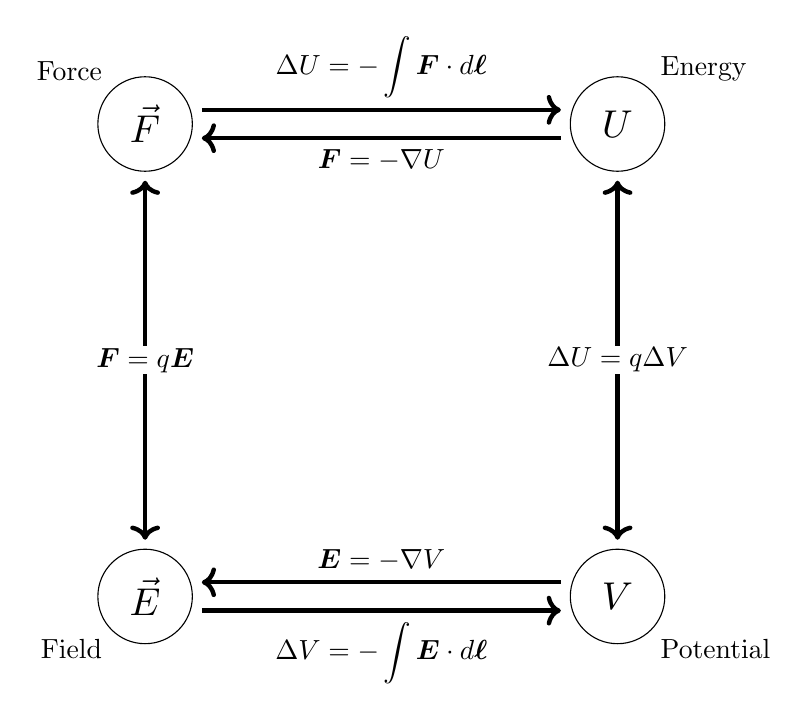
\begin{tikzpicture}[scale=0.6]
    % Nodes
    \draw[white] (5,5) -- (5.707,5.707) node[black, anchor=south west] {Energy};
    \draw[black] (5,5) circle (1);
    \node[black] at (5,5) {$\displaystyle \Scale[1.4]{U}$};
    \draw[white] (-5,5) -- (-5-0.707,5.707) node[black, anchor=south east] {Force};
    \draw[black] (-5,5) circle (1);
    \node[black] at (-5,5) {\parbox[c]{0.2\textwidth}{\begin{center} $\displaystyle \Scale[1.4]{\vec{F}}$ \end{center}}};
    \draw[white] (-5,-5) -- (-5.707,-5.707) node[black, anchor=north east] {Field};
    \draw[black] (-5,-5) circle (1);
    \node[black] at (-5,-5) {\parbox[c]{0.2\textwidth}{\begin{center} $\displaystyle \Scale[1.4]{\vec{E}}$ \end{center}}};
    \draw[white] (5,-5) -- (5.707,-5-0.707) node[black, anchor=north west] {Potential};
    \draw[black] (5,-5) circle (1);
    \node[black] at (5,-5) {\parbox[c]{0.2\textwidth}{\begin{center} $\displaystyle \Scale[1.4]{V}$ \end{center}}};
    % Top Arrow
    \draw[black, ultra thick, ->] (-3.8,5.3) -- (3.8,5.3) node[black, midway, above] {$\displaystyle \Delta U = -\int \bm{F} \cdot d\bm{\ell}$};
    \draw[black, ultra thick, <-] (-3.8,4.7) -- (3.8,4.7) node[black, midway, below] {$\displaystyle \bm{F} = -\nabla U$};
    % Bottom arrow
    \draw[black, ultra thick, ->] (-3.8,-5.3) -- (3.8,-5.3) node[black, midway, below] {$\displaystyle \Delta V = -\int \bm{E} \cdot d\bm{\ell}$};
    \draw[black, ultra thick, <-] (-3.8,-4.7) -- (3.8,-4.7) node[black, midway, above] {$\displaystyle \bm{E} = -\nabla V$};
    % Right arrow
    \draw[black, ultra thick, <-] (5,3.8) -- (5,0.3);
    \node[black] at (5,0) {$\displaystyle \Delta U = q\Delta V$};
    \draw[black, ultra thick, ->] (5,-0.3) -- (5,-3.8);
    % Left arrow
    \draw[black, ultra thick, <-] (-5,3.8) -- (-5,0.3);
    \node[black] at (-5,0) {$\displaystyle \bm{F} = q \bm{E}$};
    \draw[black, ultra thick, ->] (-5,-0.3) -- (-5,-3.8);
\end{tikzpicture}
\label{fig:3:a}
\end{figure}

Everything thus far is from intro physics, so let's start adding some new stuff. We have both
\begin{equation*}
    \nabla \cdot \bm{E} = \frac{\rho}{\epsilon_o} \qquad \text{and} \qquad \bm{E} = -\nabla V.
\end{equation*}

Substituting the latter into the former yields
\begin{equation*}
    \nabla \cdot \underbrace{\left( -\nabla V \right)}_{\displaystyle \bm{E}} = \frac{\rho}{\epsilon_o} \quad \implies \quad \boxed{\nabla^2 V = -\frac{\rho}{\epsilon_o}}
\end{equation*}

which is Poisson's equation --- the partial differential equation that yields $V$ in electrostatics given a known source $\rho$. \\

We will be solving Poisson's equation a lot in the near future, and to solve PDEs, we need boundary conditions. What might be the boundary conditions on $V$ be? \\

Well, we know
\begin{equation*}
    \Delta V = V_{\text{above}} - V_{\text{below}} = -\int \bm{E} \cdot d\bm{\ell},
\end{equation*}

and real $\bm{E}$-fields are always finite. Thus, for sufficiently small $d\bm{\ell}$, $\displaystyle \Delta V \to 0$. In other words, as the path length shrinks to zero, so too does the integral:
\begin{equation*}
    V_{\text{above}} = V_{\text{below}} \qquad \boxed{\text{So } V \text{ is always continuous.}}
\end{equation*}

That being said, we know there can be discontinuities in $\bm{E}$. And $\bm{E}$-fields come about by taking derivatives of $V$ (recall that $\bm{E} = -\nabla V$). So consider some boundary, and let $n$ denote the direction normal to the boundary (pointing from ``below'' to ``above''). We have the boundary condition on the perpendicular component of the electric field:
\begin{equation*}
    E_{\text{above}}^{\perp} - E_{\text{below}}^{\perp} = \frac{\sigma}{\epsilon_o}
\end{equation*}

Using $\displaystyle E^{\perp} = -\frac{\partial V}{\partial n}$, gives us
\begin{equation*}
    \boxed{\frac{\partial V_{\text{below}}}{\partial n} - \frac{\partial V_{\text{above}}}{\partial n} = \frac{\sigma}{\epsilon_o}}
\end{equation*}

So while $V$ is always continuous, \underline{derivatives} of $V$ aren't necessarily. At least, not the derivative perpendicular to a boundary. Since $E^{\parallel}$ is continuous, so must be the derivative of $V$ in any direction parallel to the surface. \\

(Clicker question) \\

\subsection*{Energy of a Charge Distribution}

What is the work it takes to move a charge $q$ from $\bm{x} = \bm{a}$ to $\bm{x} = \bm{b}$? We know work is given by $\displaystyle \int \bm{F} \cdot d\bm{\ell}$. The electric field exerts a force on the charge on the charge according to $\bm{F} = q\bm{E}$. Thus, the minimum force needed to overcome this field is $\bm{F} = -q\bm{E}$. It follows that the work done in moving a charge is
\begin{equation*}
    \text{Work } = \int \bm{F} \cdot d\bm{\ell} = -q \int_{\bm{a}}^{\bm{b}} \bm{E} \cdot d\bm{\ell} = q \left[ V(\bm{b}) - V(\bm{a}) \right].
\end{equation*}

Assuming we set the potential to be zero at infinity, the work required to bring in a charge from infinity to some location $\bm{x}$ is
\begin{equation*}
    \text{Work } = q \left[ V(\bm{x}) - \cancelto{0}{V(\infty)} \right] = q V(\bm{x}).
\end{equation*}

Imagine bringing a charge $q_1$ from infinity to the origin in empty space. This takes no work, since there is no field to fight against. However, once at the origin, the charge $q_1$ sets up a potential according to
\begin{equation*}
    V = \frac{1}{4\pi\epsilon_o} \frac{q_1}{\left| \bm{x} - \bm{x'} \right|} = \frac{1}{4\pi\epsilon_o} \frac{q_1}{r}.
\end{equation*}

The work done in bringing in another charge $q_2$ from infinity to some position $r$ is
\begin{equation*}
    W_{2} = q_2 \underbrace{\left( \frac{1}{4\pi\epsilon_o} \frac{q_1}{r} \right)}_{\displaystyle V} = \frac{1}{4\pi\epsilon_o} \frac{q_1 q_2}{r} \qquad\qquad \parbox[c]{0.4\textwidth}{This is the energy of interaction $U$ between two charges separated a distance $r$.}
\end{equation*}

Now we fix $q_1$ and $q_2$ in place, and let $r_{12}$ represent the distance between them. The work done in bringing in a third charge is
\begin{equation*}
    W_3 = q_3 \underbrace{\left( \frac{1}{4\pi\epsilon_o} \right) \left( \frac{q_1}{r_{13}} + \frac{q_2}{r_{23}} \right)}_{\displaystyle \text{potential from } q_1 \text{ and } q_2.}
\end{equation*}

\begin{figure}[H]
\captionsetup{width=0.8\textwidth, labelfont={color=black,bf}, textfont={color=black}}
\centering
\begin{tikzpicture}
    \filldraw[black] (0,0) circle (0.1) node[black, anchor=north west] {$q_1$};
    \draw[black, ->] (2,-1) .. controls (1.5,-1) and (0,-1) .. (0,-0.2);
    \draw[black] (0,0) -- (3,1) node[black, midway, anchor=north west] {$r_{13}$};
    \filldraw[black] (3,1) circle (0.1) node[black, anchor=north] {$q_3$};
    \draw[black, ->] (6,1) .. controls (5,1.25) and (3.5,0.75) .. (3.2,1);
    \draw[black] (3,1) -- (-2,2) node[black, midway, anchor=south west] {$r_{23}$};
    \draw[black] (0,0) -- (-2,2) node[black, midway, anchor=north east] {$r_{12}$};
    \filldraw[black] (-2,2) circle (0.1) node[black, above] {$q_2$};
    \draw[black, ->] (-5,1) .. controls (-4,2) and (-3,1) .. (-2.2,2);
\end{tikzpicture}
\label{fig:3:b}
\end{figure}

The total work in assembling these three charges is
\begin{equation*}
    W = \frac{1}{4\pi\epsilon_o} \left( \frac{q_1 q_2}{r_{12}} + \frac{q_1 q_3}{r_{13}} + \frac{q_2 q_3}{r_{23}} \right)
\end{equation*}

The work done in assembling a collection of discrete charges is also the energy we'd get if we dismantled the system. That is, it represents the energy stored in the configuration. We can generalize to $n$ number of particles:
\begin{equation*}
    U = \frac{1}{2} \left(\frac{1}{4\pi\epsilon_o}\right) \sum\limits_{i = 1}^{n} \sum\limits_{j \neq i}^{n} \frac{q_i q_j}{r_{ij}},
\end{equation*}

where the factor of $1/2$ arises because we're double counting each pair. We can re-write this expression by pulling out a factor of $q_i$ from the second sum:
\begin{equation*}
    U = \frac{1}{2} \sum\limits_{i = 1}^{n} q_i \underbrace{\left( \sum\limits_{j \neq i}^{n} \frac{1}{4\pi\epsilon_o} \frac{q_j}{r_{ij}} \right)}_{\parbox[c]{0.14\textwidth}{potential at $r_i$ (position of $q_i$) due to all other charges}} = \frac{1}{2} \sum\limits_{i = 1}^{n} q_i V
\end{equation*}

We can generalize this expression to a continuous charge distribution:
\begin{equation}
    \boxed{U = \frac{1}{2} \int \rho(\bm{x'}) V(\bm{x'})\ d^3x'} \label{eq:3:u} \tag{1}
\end{equation}

\begin{mdframed}[backgroundcolor=WHITE,align=left,userdefinedwidth=45em, topline=false, rightline=false,frametitle={Alternate derivation of (\ref{eq:3:u})}]

Start with the double sum that gives the energy of a collection of discrete charges:
\begin{equation*}
    U = \frac{1}{2} \left( \frac{1}{4\pi\epsilon_o} \right) \sum\limits_{i = 1}^{n} \sum\limits_{j \neq i}^{n} \frac{q_i q_j}{r_{ij}}
\end{equation*}

Now, instead of a collection of discrete charges, consider some continuous charge distribution, with differential charge elements $dq_1$ and $dq_2$ (located on the same charge distribution). Then the sum becomes an integral and we have
\begin{equation*}
    U = \frac{1}{2} \iint \frac{k\ dq_1\ dq_2}{r_{12}} = \frac{1}{2} \int \frac{k\ \rho(\bm{x}_1)\ \rho(\bm{x}_2)\ d^3x_1\ d^3x_2}{\left| \bm{x}_1 - \bm{x}_2 \right|}.
\end{equation*}

Again, $\rho(\bm{x}_1)$ and $\rho(\bm{x}_2)$ describe the \underline{same} charge distribution --- we're breaking the charge distribution into little $dq$'s and check each against all the others. \\

As an alternative, note that $\displaystyle \int \frac{k\ \rho(\bm{x}_1)\ d^3x_1}{\left| \bm{x}_1 - \bm{x}_2 \right|}$ is how we'd write the voltage due to $\rho$ at $\bm{x}_2$ (the location of the second charge in a particular pair). Thus, we can re-write the energy of the charge distribution as
\begin{equation*}
    U = \frac{1}{2} \int \rho(\bm{x'}) V(\bm{x'})\ d^3x'
\end{equation*}

\end{mdframed}

The expression for the energy of the system explicitly reference charge. This is not shocking --- we're used to potential energy being a thing associated with pairs of charges. But here's where it gets interesting. We're going to re-write the energy in terms of the field, thereby eliminating $\rho$ and $V$ in favor of $\bm{E}$. \\

From Gauss's law, we know that $\displaystyle \nabla \cdot \bm{E} = \frac{\rho}{\epsilon_o}$. Thus,
\begin{equation*}
    \rho = \epsilon_o \left( \nabla \cdot \bm{E} \right).
\end{equation*}

Substituting into (\ref{eq:3:u}) gives us
\begin{equation*}
    U = \frac{\epsilon_o}{2} \int \left( \nabla \cdot \bm{E} \right)\ V\ d^3x.
\end{equation*}

For any scalar-valued function $f$ and vector-valued function $\bm{A}$, the following holds:
\begin{equation*}
    \nabla \cdot \left( f \bm{A} \right) = f \left( \nabla \cdot \bm{A} \right) + \bm{A} \cdot \left( \nabla f \right).
\end{equation*}

Taking $f = V$ and $\bm{A} = \bm{E}$, we have
\begin{equation*}
    \nabla \cdot \left( V \bm{E} \right) = V \left( \nabla \cdot \bm{E} \right) + \bm{E} \cdot \left( \nabla V \right) \implies \underbrace{\left( \nabla \cdot \bm{E} \right)\ V}_{\parbox[c]{0.088\textwidth}{\begin{center} \small matches integrand above \end{center}}} = \nabla \cdot \left( V\ \bm{E} \right) - \bm{E} \cdot \left( \nabla V \right)
\end{equation*}

Substituting, we get
\begin{align*}
    U &= -\frac{\epsilon_o}{2} \int \bm{E} \cdot \underbrace{\left( \nabla V \right)}_{\displaystyle -\bm{E}} d^3x + \frac{\epsilon_o}{2} \int \nabla \cdot \left( V\ \bm{E} \right)\ d^3x \\
    &= \frac{\epsilon_o}{2} \int \underbrace{\left( \bm{E} \cdot \bm{E} \right)}_{\displaystyle E^2}\ d^3x + \frac{\epsilon_o}{2} \int \nabla \cdot \left( V\ \bm{E} \right)\ d^3x
\end{align*}

Applying the divergence theorem to the second term yields
\begin{equation*}
    U = \frac{\epsilon_o}{2} \int E^2\ d^3x + \frac{\epsilon_o}{2} \oint \left( V\ \bm{E} \right) \cdot d\bm{A}
\end{equation*}

But what volume are we integrating over? Clearly, looking at the expression for energy in (\ref{eq:3:u}), we must at least integrate over the volume that encloses our charge distribution. But what's to stop us from integrating over all space? After all, $\rho = 0$ outside the charge distribution, so the extra space contributes nothing to the integral. Then the surface integral in the second term vanishes, since it examines $V$ and $\bm{E}$ at the edge of all space (which, for any real, finite source, is zero). Thus,
\begin{equation*}
    \boxed{U = \frac{\epsilon_o}{2} \int E^2\ d^3x} \qquad\qquad \parbox[c]{0.4\textwidth}{This is entirely in terms of fields, not charge. So we can look at the fields themselves as being very real things with real energy.}
\end{equation*}

Just for fun, let's take a look at the energy associated with the field made by a point charge at the origin. The field is
\begin{equation*}
    \bm{E} = \frac{1}{4\pi\epsilon_o} \frac{q\ \rhat}{r^2}
\end{equation*}

Substituting this into the energy expression and integrating over all space yields
\begin{align*}
    U &= \frac{\epsilon_o}{2} \int \bm{E} \cdot \bm{E}\ d^3x \\
    &= \frac{\epsilon_o}{2} \left( \frac{q}{4\pi\epsilon_o} \right)^2 \int \left( \frac{\rhat}{r^2} \cdot \frac{\rhat}{r^2} \right)\ d^3x.
\end{align*}

Note that $\rhat \cdot \rhat = 1$. Taking the differential volume element to be $r^2\ \sin{\theta}\ dr\ d\theta\ d\phi$, we get
\begin{align*}
    U &= \frac{\epsilon_o}{2} \left( \frac{q}{4\pi\epsilon_o} \right)^2 \int \frac{1}{r^4} r^2\ \sin{\theta}\ dr\ d\theta\ d\phi \\
    &= \frac{\epsilon_o}{2} \left( \frac{q}{4\pi\epsilon_o} \right)^2 \underbrace{\left( \int_0^{2\pi} d\phi \right)}_{\displaystyle 2\pi} \underbrace{\left( \int_0^{\pi} \sin{\theta}\ d\theta \right)}_{\displaystyle 2} \left( \int_0^{\infty} \frac{dr}{r^2} \right) \\
    &= \frac{q^2}{8\pi\epsilon_o} \int_0^{\infty} \frac{dr}{r^2} \\
    &= \frac{q^2}{8\pi\epsilon_o} \Eval{\left( -\frac{1}{r} \right)}{0}{\infty}
\end{align*}

which kind of diverges. That's bad. \\

What we just worked shows that $\bm{E}$-fields from point charges should contain infinite energy, thereby implying that point charges shouldn't be possible. But every experiment ever done indicates that an electron is a zero-radius true point. Fixing this apparent contradiction is one of the great achievements of quantum electrodynamics.

\subsection*{Delta Functions and Point Sources}

We've already seen indications that point charges behave a bit wonky, even though they do seem to exist experimentally. I'm afraid this is going to get a bit worse before it gets better. \\

Let's take a look at Gauss's law again. If we take the divergence of an $\bm{E}$-field, we should recover the charge density that produced that field:
\begin{equation*}
    \nabla \cdot \bm{E} = \frac{\rho}{\epsilon_o}.
\end{equation*}

What happens if we take the divergence of the field made by a point charge at the origin? Applying the divergence operator in spherical coordinates gives us
\begin{equation*}
    \nabla \cdot \underbrace{\left( \frac{q}{4\pi\epsilon_o} \frac{\rhat}{r^2} \right)}_{\displaystyle \bm{E}_{\text{point}}} = \frac{1}{r^2} \frac{\partial}{\partial r} \left( \cancel{r^2} \frac{q}{4\pi\epsilon_o\ \cancel{r^2}} \right) = \frac{1}{r^2} \frac{\partial}{\partial r} \left( \frac{q}{4\pi\epsilon_o} \right) = 0\ \Scale[1.6]{?}
\end{equation*}

Well, according to that, the divergence of something like $\displaystyle \frac{\rhat}{r^2}$ is zero everywhere. Thus, so must $\rho$ be zero everywhere. But that can't be right. So what's the catch? \\

The catch is that the operator $\displaystyle \frac{1}{r^2} \frac{\partial}{\partial r} \left( r^2 \right)$ isn't super well-defined at the origin. All we can conclude from the above is that $\nabla \cdot \bm{E}$ is zero everywhere \underline{but} the origin. To deal with the origin, let's take a look at delta functions first. \\

A delta function is used to represent a finite amount of stuff compressed into an essentially zero-dimensional domain. In one dimension, a delta function $\delta(x)$ is \underline{defined} as the thingy that satisfies these two properties: $\delta(x)$ is a delta function if:

\begin{equation*}
    \displaystyle \delta(x) = \begin{cases} \displaystyle 0, & \text{if } x \neq 0 \\ \displaystyle \text{undefined}, & \text{if } x = 0 \end{cases}
\end{equation*}

and

\begin{equation*}
    \displaystyle \int \delta(x - a)\ f(x)\ dx = \begin{cases} \displaystyle f(a), & \text{if } a \text{ is in the domain of integration} \\ \displaystyle 0, & \text{otherwise} \end{cases}
\end{equation*}


Basically, it is a very sharply peaked function that, when present in an integral, plucks out the value of another function at one point:

\begin{figure}[H]
\centering
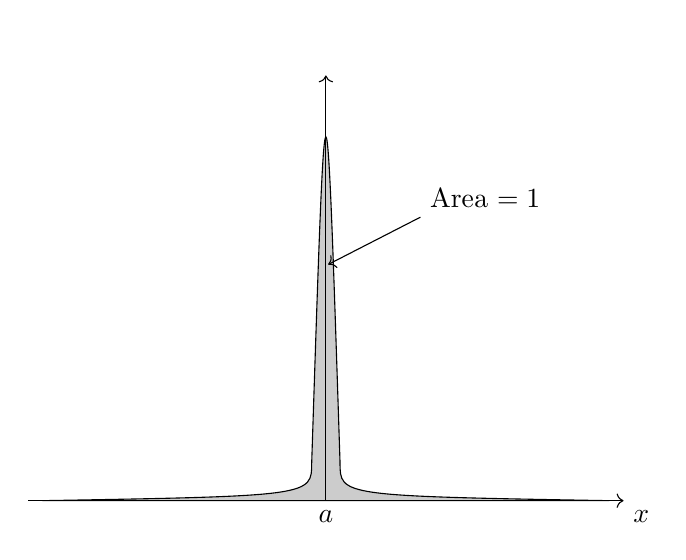
\begin{tikzpicture}[scale=0.6]
    \filldraw[color=black, fill=black!20] (-6,0) .. controls (-0.3,0.1) .. (-0.3,0.8) .. controls (0,10) .. (0.3,0.8) .. controls (0.3,0.1) .. (6,0) -- cycle;
    \draw[black, ->] (-6.3,0) -- (6.3,0) node[black, anchor=north west] {$x$};
    \draw[black, ->] (0,0) -- (0,9);
    \node[black, below] at (0,0) {$a$};
    \draw[black, <-] (0.05,5) -- (2,6) node[black, anchor=south west] {Area $= 1$};
\end{tikzpicture}
\label{fig:3:delta}
\end{figure}

So how do we represent $\rho$ for a point charge of size $q$ in 3D? How about a delta function:
\begin{equation*}
    \rho(\bm{x}) = q\ \delta^3(\bm{x}) \qquad\qquad \parbox[c]{0.33\textwidth}{(Or $\displaystyle q\ \delta^3(\bm{x} - \bm{x'})$ if the point charge is at $\bm{x'}$ instead of the origin)}
\end{equation*}

With that in mind, since $\displaystyle \nabla \cdot \bm{E} = \frac{\rho}{\epsilon_o}$, it should be the case that
\begin{equation*}
    \nabla \cdot \underbrace{\left( \frac{q}{4\pi\epsilon_o} \frac{\rhat}{r^2} \right)}_{\displaystyle \bm{E}_{\text{point}}} = \frac{1}{\epsilon_o} \underbrace{q\ \delta^3(\bm{x})}_{\displaystyle \rho}
\end{equation*}

And therefore
\begin{equation*}
    \nabla \cdot \left( \frac{\rhat}{r^2} \right) = 4\pi\delta^3(\bm{x}) \qquad\qquad \parbox[c]{0.25\textwidth}{Is this true?}
\end{equation*}

Well, it's true if
\begin{enumerate}

\item[(1)] $\displaystyle \nabla \cdot \left( \frac{\rhat}{r^2} \right) = 0$ everywhere but the origin. And we've established that.

\item[(2)] $\displaystyle \int \left( \nabla \cdot \frac{\rhat}{r^2} \right)\ d^3x = 4\pi$ for a domain of integration that includes the origin.

\end{enumerate}

Let's integrate $\displaystyle \nabla \cdot \left( \frac{\rhat}{r^2} \right)$ over a sphere of radius $R$. Just doing that as a volume integral is tricky, since the integrand is undefined at the origin, so let's dodge the bad part by using the divergence theorem:
\begin{align*}
    \int \left( \nabla \cdot \frac{\rhat}{r^2} \right)\ d^3x &= \oint \frac{\rhat}{r^2} \cdot d\bm{A} \\
    &= \oint \frac{\rhat}{r^2} \cdot \left( r^2\ \sin{\theta}\ d\theta\ d\phi\ \rhat \right) \\
    &= \oint \sin{\theta}\ d\theta\ d\phi \\
    &= \underbrace{\left( \int_0^{\pi} \sin{\theta}\ d\theta \right) \left( \int_0^{2\pi} d\phi \right)}_{\displaystyle =\ 4\pi}
\end{align*}

So it checks out. $\displaystyle \nabla \cdot \left( \frac{\rhat}{r^2} \right) = 4\pi\ \delta^3(r)$, and then
\begin{equation*}
    \nabla \cdot \left( \frac{q}{4\pi\epsilon_o} \frac{\rhat}{r^2} \right) = \frac{1}{\epsilon_o} q\ \delta^3(r) = \frac{\rho}{\epsilon_o}
\end{equation*}

and Gauss's law holds.

\newpage

\section*{Lecture 4: Multipole Expansions}
\setcounter{page}{1}

We should be getting used to the idea that we can expand complex functions in terms of simpler functions. In calculus, we learned about Taylor expansions. For $f(x)$ near $a$:
\begin{equation*}
    f(x) = f(a) + f'(a)\ (x-a) + \frac{f''(a)\ (x-a)^2}{2!} + \frac{f'''(x)\ (x-a)^3}{3!} + \cdots
\end{equation*}

which will converge more or less quickly depending of $f$ and $a$. Common Taylor series include the trig functions:
\begin{align*}
    \sin{(x)} &= x - \frac{x^3}{3!} + \frac{x^5}{5!} - \cdots \\
    \cos{(x)} &= 1 - \frac{x^2}{2!} + \frac{x^4}{4!} - \cdots
\end{align*}

You've also seen Fourier series expansions --- re-expressions of complicated functions in terms of sines and cosines:
\begin{equation*}
    f(x) = \frac{a_0}{2} + \sum\limits_{n = 1}^{\infty} a_n \cos{(nx)} + \sum\limits_{n = 1}^{\infty} b_n \sin{(nx)},
\end{equation*}

where
\begin{equation*}
    \begin{cases} \displaystyle a_0 = \int_{-\pi}^{\pi} f(x)\ dx \\[0.3cm] \displaystyle a_n = \int_{-\pi}^{\pi} f(x)\ \cos{(nx)}\ dx \\[0.3cm] \displaystyle a_n = \int_{-\pi}^{\pi} f(x)\ \sin{(nx)}\ dx \end{cases}
\end{equation*}

And there are many, many other ways to express a function in some basis. You're probably learning some general approaches in quantum right now, involving bras \& kets. \\

In electrostatics, the basic potential function for a point at the origin goes like $\displaystyle \frac{1}{r}$:
\begin{equation*}
    V_{\text{point}}(r) = \frac{k\ q}{r}.
\end{equation*}

More complicated systems (including points off the origin make more complicated potentials, but if we're decently far away we can still expand $V(\bm{x})$ as a reciprocal power series:
\begin{equation*}
    V(\bm{x}) = \frac{\text{thing}_1}{r} + \frac{\text{thing}_2}{r^2} + \frac{\text{thing}_3}{r^3} + \cdots
\end{equation*}

We call this the \underline{multipole expansion}, for reasons that will become apparent. Note that conventionally, we set this up so that $r$ is the radial coordinate, \underline{not} $\left| \bm{x} - \bm{x'} \right|$. \\

Let's start with a simple example: two point charges $q_1$ and $q_2$ at locations $\bm{x}_1$ and $\bm{x}_2$, respectively.

\begin{figure}[H]
\captionsetup{width=0.8\textwidth,labelfont={color=black,bf},textfont={color=black}}
\centering
\begin{tikzpicture}[scale=0.95]

    % Universal coordinates
    \coordinate (O) at (0,0);
    \coordinate (qone) at (0,3);
    \coordinate (qtwo) at (0,1);
    \coordinate (P) at (7.098,7.098);

    % Axis
    \draw[black, ->] (-1,0) -- (10,0);
    \draw[black, ->] (0,-1) -- (0,10);
    
    % Charges
    \filldraw[red] (qone) circle (3pt) node[red, anchor=south east] {$q_1$};
    \filldraw[red] (qtwo) circle (3pt) node[red, anchor=south east] {$q_2$};
    
    % x vectors to charges
    \draw[black, thick, ->] (O) -- (qtwo) node[black, left, pos=0.74] {$\vec{x}_1$};
    \draw[black, thick, ->] (qtwo) -- (qone) node[black, left, midway] {$\vec{x}_2$};
    
    % Observer
    \filldraw[black] (P) circle (1pt) node[black, anchor=south west] {$P$};
    
    % x
    \draw[black, thick, ->] (O) -- (P) node[black, pos=0.6, anchor=north west] {$\vec{x}$};
    
    % x - x1
    \draw[black, thick, ->] (qone) -- (P) node[black, midway, anchor=south east] {$\vec{x} - \vec{x}_1$};
    
    % theta
    \draw[black, <->] (0,1.6) arc (90:45:1.6) node[black, midway, anchor=south] {$\theta$};
    
    % Description
    \node[black] at (12,4) {\parbox[c]{0.4\textwidth}{\begin{center} We want to find the voltage at point $P$, which is at some arbitrary angle $\theta$. \end{center}}};
    
\end{tikzpicture}
\caption*{I'll let the $\theta = 0$ axis lay along the line that includes the charges. Additionally, let $\left| \bm{x} \right| = r$, $\left| \bm{x}_1 \right| = r_1$, and $\left| \bm{x}_2 \right| = r_2$. We're interested in the r{\'e}gime where $r \gg r_1 + r_2$ (point $P$ is far from the charges).}
\label{fig:4:dipole}
\end{figure}

The exact expression for the voltage at $P$ is
\begin{equation}
    V(\bm{x}) = \frac{1}{4\pi\epsilon_o} \frac{q_1}{\left| \bm{x} - \bm{x}_1 \right|} + \frac{1}{4\pi\epsilon_o} \frac{q_2}{\left| \bm{x} - \bm{x}_2 \right|} \tag{1} \label{eq:4:exact}
\end{equation}

Consider the triangle formed above:


\begin{figure}[H]
\captionsetup{width=0.8\textwidth,labelfont={color=black,bf},textfont={color=black}}
\centering
\begin{tikzpicture}[scale=0.8]

    % Universal coordinates
    \coordinate (O) at (0,0);
    \coordinate (qone) at (0,3);
    \coordinate (qtwo) at (0,1);
    \coordinate (P) at (7.098,7.098);
    
    % Charges
    \filldraw[red] (qone) circle (3pt) node[red, anchor=south east] {$q_1$};
    % \filldraw[red] (qtwo) circle (3pt) node[red, anchor=south east] {$q_2$};
    
    % r to charge
    % \draw[black, thick, ->] (O) -- (qtwo) node[black, left, pos=0.74] {$\vec{x}_1$};
    \draw[black, thick] (O) -- (qone) node[black, midway, left] {$r_1$};
    %\draw[black, thick, decoration={brace, raise=5pt}, decorate] (O) -- (qone) node[black, midway, left=6pt] {$r_1$};
    
    % Observer
    \filldraw[black] (P) circle (1pt) node[black, anchor=south west] {$P$};
    
    % xr
    \draw[black, thick] (O) -- (P) node[black, midway, anchor=north west] {$r$};
    %\draw[black, thick, decoration={brace, raise=5pt, mirror}, decorate] (O) -- (P) node[black, pos=0.57, anchor=north east, below=14pt] {$r$};
    
    % x - x1
    \draw[black, thin] (qone) -- (P);
    \draw[black, thick, decoration={brace, raise=5pt}, decorate] (qone) -- (P) node[black, midway, above=6pt, anchor=south east] {$\left| \vec{x} - \vec{x}_1 \right|$};
    
    % theta
    \draw[black, <->] (0,1.6) arc (90:45:1.6) node[black, midway, anchor=south] {$\theta$};
    
    % Description
    \node[black] at (13,4) {\parbox[c]{0.4\textwidth}{\begin{center} Using the law of cosines, we have \\ $\displaystyle \left| \bm{x} - \bm{x}_1 \right|^2 = r^2 + r_1^2 - 2r r_1\ \cos{\theta}$ \end{center}}};
    
\end{tikzpicture}
\label{fig:4:triangle}
\end{figure}

Expanding the denominator of the first term of (\ref{eq:4:exact}) gives us
\begin{equation*}
    \frac{1}{\left| \bm{x} - \bm{x}_1 \right|} = \frac{1}{\sqrt{r^2 - 2rr_1 \cos{\theta} + r_1^2}}
\end{equation*}

Pulling out a $1/r$,
\begin{gather*}
    \frac{1}{\left| \bm{x} - \bm{x}_1 \right|} = \frac{1}{\sqrt{r^2 \left( 1 + \frac{r_1^2 - 2rr_1\ \cos{\theta}}{r^2} \right)}} = \frac{1}{r\ \sqrt{1 + \frac{r_1^2 - 2rr_1\ \cos{\theta}}{r^2}}} = \frac{1}{r} \underbrace{\left( 1 + \frac{r_1^2 - 2r r_1\ \cos{\theta}}{r^2} \right)^{-1/2}}_{\displaystyle \left( 1 + \text{small} \right)^n}
\end{gather*}

We can use a binomial expansion on the term in parentheses. The general formula is
\begin{equation*}
    \left( 1 + x \right)^{-1/2} = 1 - nx + \frac{n(n + 1)}{2!} x^2 - \frac{n(n+1)(n+2)}{3!}x^3 + \cdots,
\end{equation*}

or by taking $n = 1/2$,
\begin{equation*}
    \left( 1 + x \right)^{-1/2} = 1 - \frac{1}{2}x + \frac{3}{8}x^2 - \cdots
\end{equation*}

which converges absolutely for $|x| < 1$. Here, we take $\displaystyle x = \frac{r_1^2 - 2rr_1\ \cos{\theta}}{r^2}$. Since $r \gg r_1$, the convergence condition is satisfied. Thus, we have
\begin{align*}
    \frac{1}{\left| \bm{x} - \bm{x}_1 \right|} &\simeq \frac{1}{r} \left[ 1 + \frac{1}{2} \frac{2rr_1\ \cos{\theta} - r_1^2}{r^2} + \frac{3}{8} \left( \frac{4r^2 r_1^2\ \cos^2{\theta} - 4r r_1^3\ \cos{\theta} + r_1^4}{r^4} \right) \right] \\
    &= \frac{1}{r} + \frac{r_1\ \cos{\theta}}{r^2} - \frac{r_1^2}{2r^3} + \frac{3}{2} \frac{r_1^2\ \cos^2{\theta}}{r^3} - \frac{3}{2} \frac{r_1^3\ \cos{\theta}}{r^4} + \frac{3}{8} \frac{r_1^4}{r^5}.
\end{align*}

Again, we're interested the potential far away from the point charges (so $r \gg r_1$), meaning we can safely drop all terms higher order than $1/r^3$. Moreover, since we're far away, the angle $\theta$ for the different sources are about the same. As such, we can follow an identical process for the second term in (\ref{eq:4:exact}), thereby giving us
\begin{equation*}
    \frac{1}{\left| \bm{x} - \bm{x}_2 \right|} = \frac{1}{r} + \frac{r_2\ \cos{\theta}}{r^2} - \frac{r_2^2}{2r^3} + \frac{3}{2} \frac{r_2^2\ \cos^2{\theta}}{r^3}
\end{equation*}

Superposition gives us the voltage at $P$:
\begin{equation*}
    V(r,\theta) = \frac{1}{4\pi\epsilon_o} \left[ \underbrace{\frac{q_1 + q_2}{r}}_{\displaystyle \text{monopole}} + \underbrace{\frac{\left( q_1 r_1 + q_2 r_2 \right)\ \cos{\theta}}{r^2}}_{\displaystyle \text{dipole}} + \underbrace{\frac{q_1 r_1^2 + q_2r_2^2}{2r^3} \left( 3\cos^2{\theta} - 1 \right)}_{\displaystyle \text{quadrupole}} \right]
\end{equation*}

Note the presence of three terms (to wit: the monopole, dipole, and quadrupole terms). Physically, we interpret them as follows: \\

A \textbf{monopole} (a point charge) makes a voltage that goes like $1/r$ (and a field like $1/r^2$). A system of charges has a term in its voltage that goes like $k q_{\text{tot}}/r$, where $q_{\text{tot}}$ is the total charge of the system. \\

A standard \textbf{dipole} is two charges of the same magnitude $q$ and opposite sign, separated by some distance $d$.

The net charge of a true dipole is zero (no monopole moment), so far away it has \underline{no} $1/r$ potential. It does, however, have some leftover $1/r^2$ potential. The equal \& opposite charges screen away some, but not all, of $V$.

The dipole moment of this pair is defined as
\begin{equation*}
    \bm{p} \equiv q \bm{d}
\end{equation*}

and its potential far away looks like
\begin{equation*}
    V(\bm{x}) = \frac{\bm{p} \cdot \rhat}{4\pi\epsilon_o\ r^2}
\end{equation*}

And a general definition for the dipole moment of any charge is $\displaystyle \bm{p} = q\bm{x'}$, where $\bm{x'}$ is the location of the charge.

So something that looks like $\displaystyle \frac{q r \cos{\theta}}{r^2}$ is exactly a dipole potential.

\begin{figure}[H]
\centering
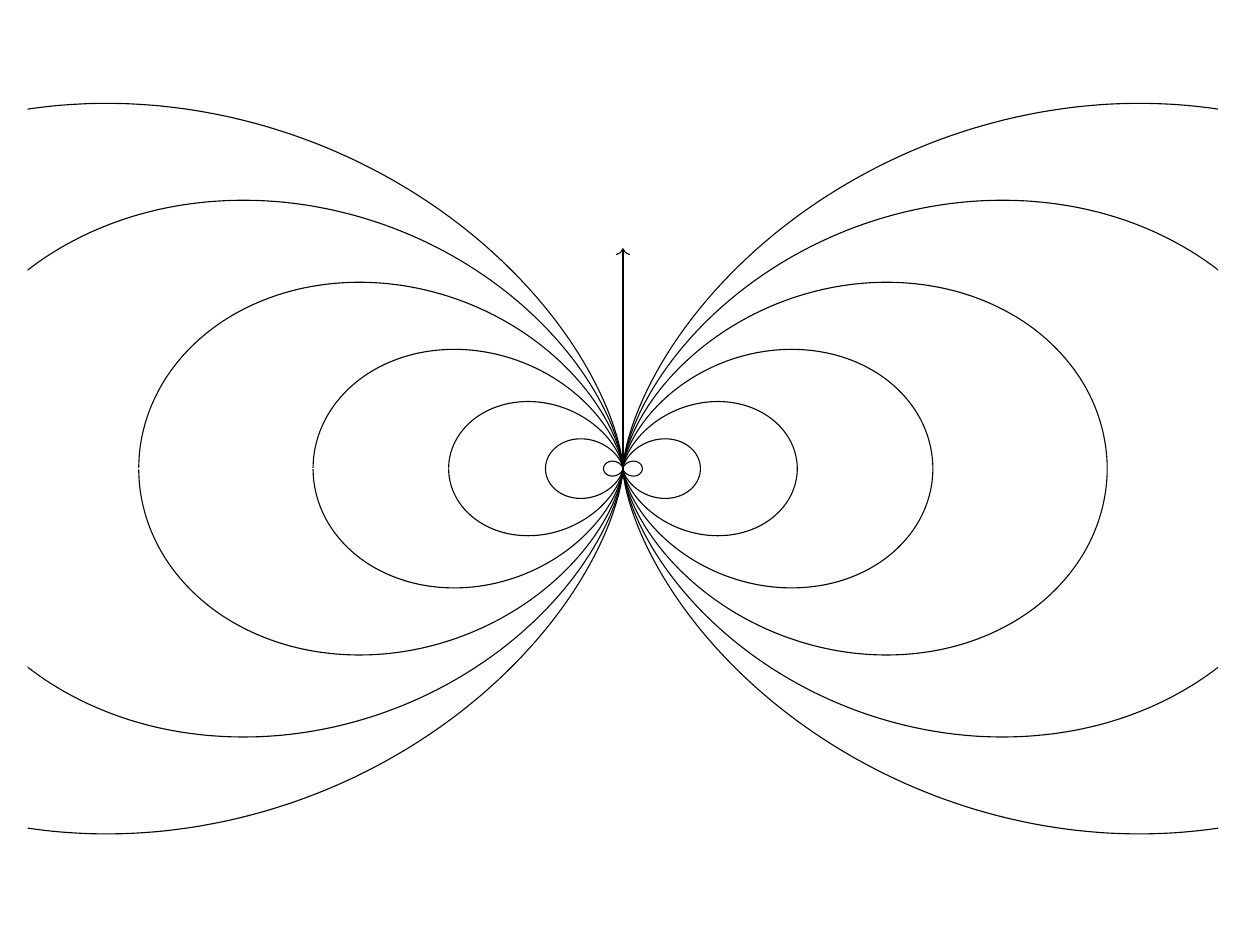
\begin{tikzpicture}[scale=1.4]
    \clip (-5.4,-4) rectangle (5.4,4);
    \foreach \u in {0,...,7}
    \draw[color=black, domain=-3.14:3.14, samples=200, smooth] plot (canvas polar cs:angle=\x r,radius={\u*cos(\x r)*\u*cos(\x r)*5});
    \draw[black, ->] (0,0) -- (0,2);
\end{tikzpicture}
\label{fig:4:exactdipole}
\end{figure}

\begin{minipage}{0.4\textwidth}
\begin{flushleft}
\begin{figure}[H]
\captionsetup{width=0.8\textwidth,labelfont={color=black,bf},textfont={color=black}}
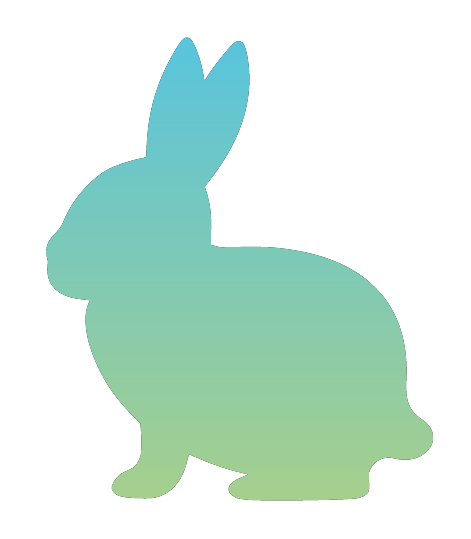
\begin{tikzpicture}
    \node at (0,0) {\bunny[scale=2.5, top color=BLUE_C, bottom color=GREEN_B]};
\end{tikzpicture}
\label{fig:4:water}
\end{figure}
\end{flushleft}
\end{minipage}
\hspace{-1cm}
\begin{minipage}{0.6\textwidth}
\begin{flushright}
\parbox[c]{\textwidth}{\begin{flushleft} Note that most molecules are polar to some degree. For instance, the water molecule has the dipole moment $\bm{p}$ shown. You can find tables of dipole moments easily enough. \end{flushleft}}
\end{flushright}
\end{minipage}

A \underline{quadrupole} is two dipoles back to back in such a way that their dipole moments cancel, as do their voltages that go like $1/r^2$, leaving $1/r^3$ as a remainder.

We've seen quadrupoles before in field session (mass spectrometry unit).

Deriving an expression for the potential of a quadrupole takes a bit more work but is essentially what we did before. For now, take my word for it that the third term in (1) is a quadrupole-like term.

So now we can see what a multipole expansion is, physically. We're expanding a potential function is a basis, where the elements of the basis include the kinds of fields made by a monopole, a dipole, a quadrupole, and so on. \\

What we did with the two charge system above is generalizable. For any localized charge distribution, if we're far from the source,
\begin{equation*}
    V(\bm{x}) \simeq \frac{1}{4\pi\epsilon_o} \left[ \frac{Q_{\text{net}}}{r} + \frac{\rhat \cdot \bm{p}}{r^2} + \frac{}{} \right]
\end{equation*}

\newpage

\section*{Lecture 5: Conductors, Capacitors, and the Method of Images}
\setcounter{page}{1}

Coulomb's law gives us a recipe for finding the electric field anywhere in space given a static distribution of charge. This includes charges on insulating material. \\

But what if we add conductors? Charges can shift around and so now we don't know $\rho(\bm{x})$ everywhere ahead of time. What now? \\

Now, we learn how to solve Poisson's equation, $\displaystyle \nabla^2 V = -\frac{\rho}{\epsilon_o}$. A lot. \\

First, some properties of conductors:

\begin{enumerate}

\item[(1)] (Some) charges are free to move.

\item[(2)] Charges exist in vast numbers, even if the net charge is zero.

\item[(3)] The electric field $\bm{E}$ is zero in a conductor in electrostatic equilibrium. Achieving electrostatic equilibrium takes very little time, about \SI{10e-19}{\second} in copper (which is effectively zero)

\begin{enumerate}

\item[(3a)] Voltages in conductors are constant, since $\displaystyle \Delta V = \int \bm{E} \cdot d\bm{\ell} = 0$

\end{enumerate}

\item[(4)] Inside a conductor, $\displaystyle \rho(\bm{x}) = 0$. This follows from Gauss's law.

\begin{enumerate}

\item[(4a)] Net charges therefore live on the surface.

\end{enumerate}

\item[(5)] At the surface of a conductor, $\displaystyle E^{\parallel} = 0$ and $E^{\perp} = \frac{\sigma}{\epsilon_o}$. This is a special (and most relevant) case of our old boundary condition.

Note that this is absolute and very powerful: if we know $\sigma$ at the surface of a conductor we know $\bm{E}$ and vice-versa.

\end{enumerate}

This is all stuff we can infer without much in the way of mathematical hardware. But to move on we need more.

\begin{equation*}
    \begin{rcases} \text{Poisson's equation:} \quad \nabla^2 V = -\frac{\rho}{\epsilon_o} \\[0.5cm] \displaystyle \text{Laplace's equation:} \quad \nabla^2 V = 0 \end{rcases} \qquad \parbox[c]{0.5\textwidth}{And these have \underline{unique} solutions, as long as we know all the boundary conditions --- just like we got used to in diffy q.}
\end{equation*}

We can use this information on the uniqueness of solutions to prove something I stated as fact in Phys 200.

\begin{enumerate}

\item[(6)] Given any chunk of conductor with any kind of cavity (hollow) in electrostatic equilibrium, $\bm{E} = \bm{0}$ in the cavity.

\begin{proof}

Since there is no charge inside the cavity, we must satisfy $\displaystyle \nabla^2 V = 0$. The edge of the cavity are at some constant potential, $V_o$ (boundary condition).

Guess a solution: $V = V_o$ throughout the cavity. This satisfies $\displaystyle \nabla^2 V = 0$ and the boundary condition, so it's a solution to Laplace's equation. But Laplace's equation only admits \underline{unique} solutions. So $V = V_o$ in the cavity (and hence $\bm{E} = \bm{0}$ is \underline{the} solution.

\end{proof}

\item[(7)] Extending this further, we can discover that even if the conductor has charge, a hollow will have no charge on the interior surface.

\end{enumerate}

So what makes a conductor a conductor? (Periodic table slide) The theory of conduction (band theory) is quantum mechanical in nature and is coming up soon (Griffiths 5.3). Keep an eye out! \\

Now let's get back to the general problem of solving Laplace's equation with conductors. \\

We will start with two ``large" $\displaystyle \left( \sqrt{\text{Area}} \gg d \right)$ square metal plates, the prototypical capacitor. Ground one plate $\displaystyle (V = 0)$ and hold the other at some $V_o$ (these are our boundary conditions). Let's even let the plates have thicknesses, $d_1$ and $d_2$.

\begin{figure}[H]
\captionsetup{width=0.8\textwidth}
\centering
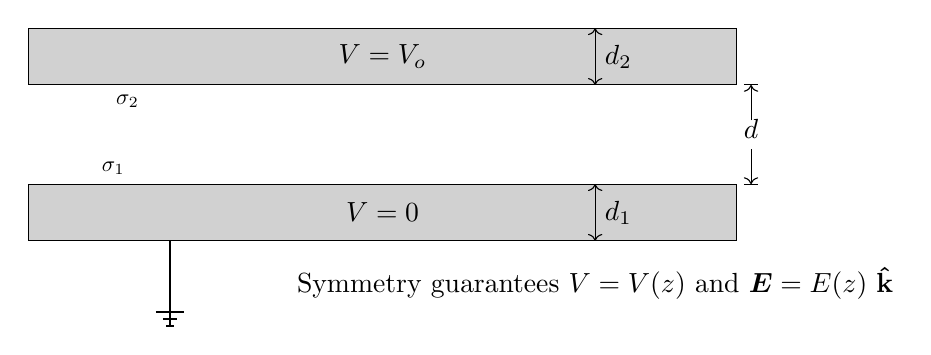
\begin{tikzpicture}[scale=0.9]

    % Bottom metal plate
    \filldraw[color = black, fill = black!18] (0,0) rectangle (10,0.8);
    \node[black] at (5,0.4) {$V = 0$};
    \draw[black, <->] (8,0) -- (8,0.8) node[black, midway, right] {$d_1$};
    
    % Ground
    \draw[black] (2,0) -- (2,-1.2);
    \draw[black, thick] (1.8,-1) -- (2.2,-1);
    \draw[black, thick] (1.9,-1.1) -- (2.1,-1.1);
    \draw[black, thick] (1.95,-1.2) -- (2.05,-1.2);
    
    % symmetry guarantees
    \node[black] at (8,-0.6) {Symmetry guarantees $V = V(z)$ and $\bm{E} = E(z)\ \khat$};
    
    % Top metal plate
    \filldraw[color = black, fill = black!18] (0,2.2) rectangle (10,3);
    \node[black] at (5,2.6) {$V = V_o$};
    \draw[black, <->] (8,2.2) -- (8,3) node[black, midway, right] {$d_2$};
    
    % Thickness d
    \draw[black] (10.1,0.8) -- (10.3,0.8);
    \draw[black] (10.1,2.2) -- (10.3,2.2);
    \draw[black, <-] (10.2,0.8) -- (10.2,1.3)  node[black, above] {$d$};
    \draw[black, ->] (10.2,1.7) -- (10.2,2.2);
    
    % sigma 1
    \node[black, above] at (1.2,0.8) {$\Scale[0.8]{\sigma_1}$};
    
    % sigma 2
    \node[black, below] at (1.4,2.2) {$\Scale[0.8]{\sigma_2}$};
    
\end{tikzpicture}
\label{fig:5_:cap}
\end{figure}

In between the plates Laplace's equation ($\nabla^2 V = 0$) applies (since there can't be any charge there), so let's guess and check. Taking $V = \text{constant}$ won't satisfy the boundary conditions, but a linear potential ($\displaystyle V = c_1 z + c_2$, where $c_1$ and $c_2$ are constants) will. So let's guess
\begin{gather*}
    V(z) = \frac{V_o}{d} z \qquad\qquad \parbox[c]{0.5\textwidth}{This fits the boundary conditions and satisfies Laplace's equation, so it must be the unique solution} \\[0.2cm]
    \implies \bm{E} = -\frac{V_o}{d}\ \khat
\end{gather*}

That was easy. Now, can we infer the surface charge densities $\sigma_1$ and $\sigma_2$ on the interior sheets? Well, for conductors, we have the boundary condition
\begin{equation*}
    \bm{E} = \frac{\sigma}{\epsilon_o} \nhat \qquad \text{at an edge.}
\end{equation*}

Recall that the unit normal vector always points outward from a surface. So for the bottom plate (surface 1), the unit normal vector is $\nhat_1 = \khat$ and
\begin{equation*}
    \bm{E}_1 = \frac{\sigma_1}{\epsilon_o} \khat = -\frac{V_o}{d} \khat \quad \implies \quad \sigma_1 = -\frac{V_o \epsilon_o}{d}.
\end{equation*}

Once the unit normal vector is defined, it is signed. So since the unit normal vector points outward from the top plate (surface 2), we take $\nhat_2 = -\khat$ and
\begin{equation*}
    \bm{E}_2 = -\frac{\sigma_2}{\epsilon_o} \khat = -\frac{V_o}{d}\khat \quad \implies \quad \sigma_2 = \frac{V_o \epsilon_o}{d}.
\end{equation*}

In the regions above and below


\newpage

\section*{Lecture 6: Spherical Symmetry}
\setcounter{page}{1}


\newpage

\section*{Lecture 7: Cylindrical Symmetry}
\setcounter{page}{1}


\newpage

\section*{Lecture 8: Separation of Variables, Hyperbolic Functions, and Series Solutions}
\setcounter{page}{1}

Suppose we have a non-trivial differential equation like, oh I don't know, Laplace's equation:
\begin{equation*}
    \nabla^2 V = \frac{\partial^2 V}{\partial x^2} + \frac{\partial^2 V}{\partial y^2} + \frac{\partial^2 V}{\partial z^2} = 0.
\end{equation*}
We've learned methods for highly symmetric cases and gimmicks for a few others, but no general techniques. We're going to use separation of variables and series solutions to learn how to solve Laplace's equation for \underline{any} configuration. \\

Assume a solution of the form of products:
\begin{equation*}
    V(x, y, z) = X(x) Y(y) Z(z).
\end{equation*}

This looks like a severe constraint, but we get lucky and solutions of this form are such that linear combinations of multiple solutions can be used to build up anything else. That is, the solutions will form a \underline{complete set} (span the space of functions). Let's take our ansatz ($V(x, y, z) = X(x) Y(y) Z(z)$) and substitute it into Laplace's equation:
\begin{equation*}
    YZ \frac{d^2 X}{dx^2} + XZ \frac{d^2 Y}{dy^2} + XY \frac{d^2 Z}{dz^2} = 0.
\end{equation*}

Dividing both sides by $V(x,y,z) = X(x) Y(y) Z(z)$ gives
\begin{equation*}
    \underbrace{\frac{1}{X} \frac{d^2 X}{dx^2}}_{\parbox[c]{0.1\textwidth}{\centering depends only on $x$}} + \underbrace{\frac{1}{Y} \frac{d^2 Y}{dy^2}}_{\parbox[c]{0.1\textwidth}{\centering depends only on $y$}} + \underbrace{\frac{1}{Z} \frac{d^2 Z}{dz^2}}_{\parbox[c]{0.1\textwidth}{\centering depends only on $z$}} = \quad 0.
\end{equation*}

Notice how each term is independent (that is, this equation assumes the form $f(x) + g(y) + h(z) = 0$). Then the only way for this equation to hold is for each term individually to be a constant. (Fiddling with $x$, say, while holding $y$ and $z$ constant must leave the sum of the three terms untouched at zero --- this implies $f(x)$ is constant). So we have
\begin{equation*}
    \frac{1}{X} \frac{d^2 X}{dx^2} = \kappa_1^2, \qquad \frac{1}{Y} \frac{d^2 Y}{dy^2} = \kappa_2^2, \qquad \text{and} \qquad \frac{1}{Z} \frac{d^2 Z}{dz^2} = \kappa_3^2 \qquad \parbox[c]{0.2\textwidth}{with the constraint $\kappa_1^2 + \kappa_2^2 + \kappa_3^2 = 0$.}
\end{equation*}

We just turned a single PDE in three variables into three ODEs. Notice that the ODEs are the same ones that describe a simple harmonic oscillator. The general solutions to these ODEs is
\begin{equation*}
    \begin{cases} \displaystyle X(x) = C_1 e^{\kappa_1 x} + D_1 e^{-\kappa_1 x} \\[0.4cm] \displaystyle Y(y) = C_2 e^{\kappa_2 y} + D_2 e^{-\kappa_2 y} \\[0.4cm] \displaystyle Z(z) = C_3 e^{\kappa_3 z} + D_3 e^{-\kappa_3 z} \end{cases}
\end{equation*}

where the separation constants $\kappa_1$, $\kappa_2$, and $\kappa_3$ are complex numbers.

\begin{mdframed}[backgroundcolor=white, align=left, userdefinedwidth=\textwidth, topline=false, bottomline = false, rightline = false, frametitle = {An interlude: Trigonometric and Hyperbolic Functions.}]

Trigonometric and hyperbolic functions have similar structure and behavior. Both are composed of exponential functions. Hyberbolic functions use reals, trigonometric use complex:
\begin{gather*}
    \sin{(x)} = \frac{e^{ix} - e^{-ix}}{2i}, \qquad \sinh{(x)} = \frac{e^x - e^{-x}}{2} \\
    \cos{(x)} = \frac{e^{ix} + e^{-ix}}{2}, \qquad \cosh{(x)} = \frac{e^x + e^{-x}}{2}.
\end{gather*}

Why bother with these functions at all instead of using $\left\{ e^x, e^{-x}, e^{ix}, e^{-ix} \right\}$ as our basic set? \\

Trigonometric ($\sin{(x)}$ and $\cos{(x)}$) and hyperbolic ($\sinh{(x)}$ and $\cosh{(x)}$) functions are constructed to be even or odd. You can think of them as the even and odd ``components" of the exponentials:
\begin{align*}
    e^{ix} &= \cos{x} + i \sin{x} \\
    e^x &= \cosh{x} + \sinh{x}
\end{align*}

Here are some graphs:

\begin{minipage}{0.5\textwidth}
\begin{flushleft}
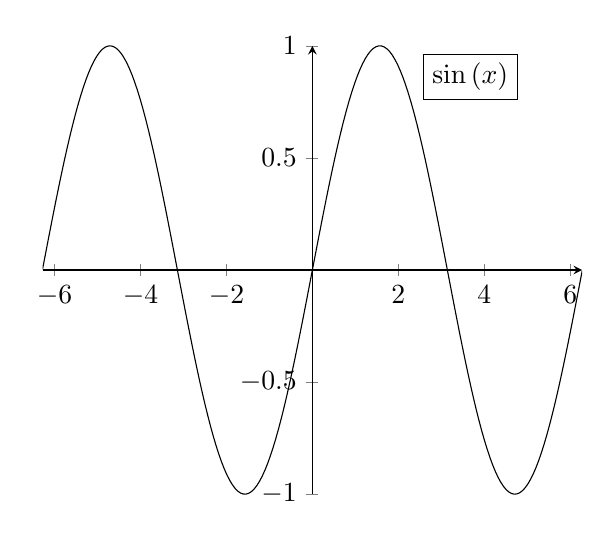
\begin{tikzpicture}
    \begin{axis}[axis lines = middle]
    \addplot[domain=-6.28:6.28, samples=200, color=black]{sin(deg(x))} node[black, pos=0.68, anchor=south west] {$\boxed{\sin{(x)}}$};
    %\addlegendentry{$\sin{(x)}$}
    \end{axis}
\end{tikzpicture}
\end{flushleft}
\end{minipage}
~
\begin{minipage}{0.5\textwidth}
\begin{flushright}
\begin{tikzpicture}
    \begin{axis}[axis lines = middle, restrict y to domain=-12:12]
    \addplot[domain=-2.5:2.5, samples=200, color=black]{sinh(x)} node[black, pos=0.86, anchor=south east] {$\boxed{\sinh{(x)}}$};
    %\addlegendentry{$\sinh{(x)}$}
    \end{axis}
\end{tikzpicture}
\end{flushright}
\end{minipage}

\begin{minipage}{0.5\textwidth}
\begin{flushleft}
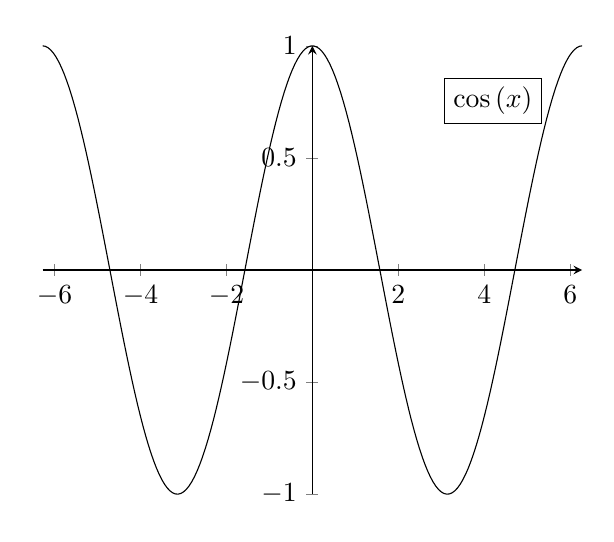
\begin{tikzpicture}
    \begin{axis}[axis lines = middle]
    \addplot[domain=-6.28:6.28, samples=200, color=black]{cos(deg(x))} node[black, pos=0.95, anchor=east] {$\boxed{\cos{(x)}}$};
    %\addlegendentry{$\cos{(x)}$}
    \end{axis}
\end{tikzpicture}
\end{flushleft}
\end{minipage}
~
\begin{minipage}{0.5\textwidth}
\begin{flushright}
\begin{tikzpicture}
    \begin{axis}[axis lines = middle, restrict y to domain=-12:12]
    \addplot[domain=-2.5:2.5, samples=200, color=black]{cosh(x)} node[black, pos=0.95, anchor=east] {$\boxed{\cosh{(x)}}$};
    %\addlegendentry{$\cosh{(x)}$}
    \end{axis}
\end{tikzpicture}
\end{flushright}
\end{minipage}

\begin{minipage}{0.5\textwidth}
\begin{flushleft}
\begin{tikzpicture}[scale=0.36]
    % Using r=6.6
    \draw[black, ->] (0,-10) -- (0,10) node[black, above] {$\Im (z)$};
    \draw[black, ->] (-10,0) -- (10,0) node[black, right] {$\Re (z)$};
    \draw[black] (0,0) circle (6.6);
    \coordinate (z) at (3.3,5.71577);
    \coordinate (x) at (3.3,0);
    \coordinate (y) at (3.3,2.85788);
    \draw[black] (0,0) -- (z) -- (x);
    \draw[black, decoration={brace, mirror, raise=5pt}, decorate] (0,0) -- (x) node[black, midway, below=6pt] {$\cos{\theta}$};
    \node[black, right] at (y) {$\sin{\theta}$};
    \filldraw[black] (z) circle (2pt) node[black, anchor=south west] {$e^{i\theta} = \cos{\theta} + i\sin{\theta}$};
    \draw[black, <->] (1.8,0) arc (0:60:1.8) node[black, midway, anchor=south west] {$\theta$};
\end{tikzpicture}
\end{flushleft}
\end{minipage}
~
\begin{minipage}{0.5\textwidth}
\begin{flushright}
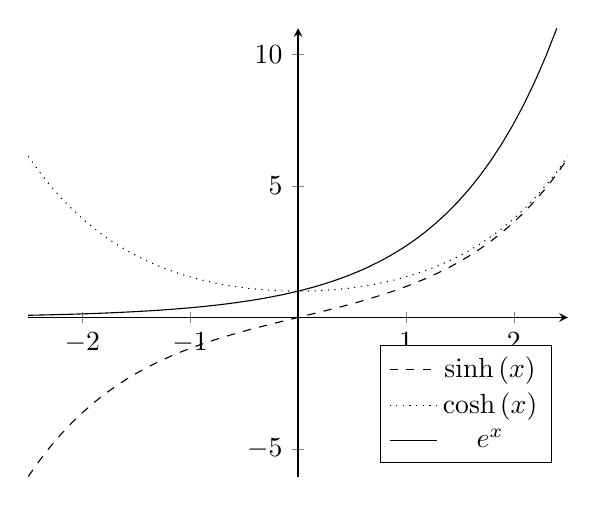
\begin{tikzpicture}
    \begin{axis}[axis lines = middle, restrict y to domain=-12:12, legend pos=south east]
    \addplot[domain=-2.5:2.5, samples=50, color=black, dashed]{sinh(x)};
    \addlegendentry{$\sinh{(x)}$}
    \addplot[domain=-2.5:2.5, samples=50, color=black, dotted]{cosh(x)};
    \addlegendentry{$\cosh{(x)}$}
    \addplot[domain=-2.5:2.5, samples=50, color=black]{e^x};
    \addlegendentry{$e^x$}
    \end{axis}
\end{tikzpicture}
\end{flushright}
\end{minipage}

\end{mdframed}

In short, trigonometric and hyperbolic functions are basically rewrites of exponential functions and have some pleasant properties. So we use them to build up our solutions to Laplace's equations. So the general solution to $\displaystyle \frac{d^2 X}{dx^2} = \kappa^2 X$ is
\begin{equation*}
    X(x) = A e^{\kappa x} + B e^{-\kappa x} \qquad \Longleftrightarrow \qquad X(x) =  \begin{cases} \displaystyle C_1 \cosh{(\kappa x)} + C_2 \sinh{(\kappa x)}, & \text{if } \kappa \text{ is real} \\[0.4cm] \displaystyle C_1 \cos{(\kappa x)} + C_2 \sin{(\kappa x)}, & \text{if } \kappa \text{ is imaginary} \end{cases}
\end{equation*}

Now, Laplace's equation is \underline{linear}, so any combination of solutions is also a solution. So our general approach will be to use a \underline{series} solution. Perhaps something like
\begin{equation*}
    V(x, y) = \sum\limits_{n = 0}^{\infty} V_n \sin{\left( \frac{n \pi x}{L} \right)} \cosh{\left( y \right)}.
\end{equation*}

Remember from Fourier analysis: sines and cosines are \underline{orthogonal} functions. That means for any symmetric interval of length $2L$, the following hold:
\begin{align*}
    \int_{-L}^{L} \sin{\left( \frac{n\pi x}{L} \right)} \sin{\left( \frac{n\pi x}{L} \right)}\ dx &= \begin{cases} \displaystyle 2L, & m = n = 0 \\ \displaystyle L, & m = n \neq 0 \\ \displaystyle 0, & m \neq n \end{cases} \\
    \int_{-L}^{L} \cos{\left( \frac{n\pi x}{L} \right)} \cos{\left( \frac{n\pi x}{L} \right)}\ dx &= \begin{cases} \displaystyle L, & m = n \\ \displaystyle 0, & m \neq n \end{cases} \\
    \int_{-L}^{L} \sin{\left( \frac{n\pi x}{L} \right)} \cos{\left( \frac{n\pi x}{L} \right)}\ dx &= 0,
\end{align*}

where $n, m$ are integers. Orthogonality allows us to find the Fourier series of a known function, say $f$, over some interval (here, on $-L < x < L$):
\begin{equation*}
    f(x) = \frac{a_o}{2} + \sum\limits_{n = 1}^{\infty} \left[ a_n \cos{\left( \frac{n\pi x}{L} \right)} + b_n \sin{\left( \frac{n\pi x}{L} \right)}  \right]
\end{equation*}

Let's multiply both sides by $\sin{\left( \frac{m\pi x}{L} \right)}$ and integrate from $-L$ to $L$. Doing so gives
\begin{align*}
    \int_{-L}^{L} f(x)\ \sin{\left( \frac{m\pi x}{L} \right)}\ dx &= \int_{-L}^{L} \left[ \frac{a_o}{2} \sin{\left( \frac{m\pi x}{L} \right)} \right]\ dx\ +\ \int_{-L}^{L} \left[ \sum_{n=1}^{\infty} a_n \cos{\left( \frac{n\pi x}{L} \right)} \sin{\left( \frac{m\pi x}{L} \right)} \right]\ dx \\
    &\qquad\qquad +\ \int_{-L}^{L} \left[ \sum_{n=1}^{\infty} b_n \sin{\left( \frac{n\pi x}{L} \right)} \sin{\left( \frac{m\pi x}{L} \right)} \right]\ dx
\end{align*}

Interchanging the sum and the integral,
\begin{align*}
    \int_{-L}^{L} f(x)\ \sin{\left( \frac{m\pi x}{L} \right)}\ dx &= \cancelto{0}{\frac{a_o}{2} \int_{-L}^{L} \sin{\left( \frac{m\pi x}{L} \right)}\ dx}\ +\ \sum_{n = 1}^{\infty} a_n \cancelto{0}{\int_{-L}^{L} \cos{\left( \frac{n\pi x}{L} \right)} \sin{\left( \frac{m\pi x}{L} \right)}\ dx} \\
    &\qquad\qquad +\ \sum_{n = 1}^{\infty} b_n \int_{-L}^{L} \sin{\left( \frac{n\pi x}{L} \right)} \sin{\left( \frac{m\pi x}{L} \right)}\ dx.
\end{align*}

The first two terms vanish for all integer $m$ and $n$. The last term vanishes if $m \neq n$. So we have
\begin{equation*}
    \int_{-L}^{L} f(x)\ \sin{\left( \frac{m\pi x}{L} \right)}\ dx = \sum_{n = 1}^{\infty} b_n \underbrace{\int_{-L}^{L} \sin{\left( \frac{n\pi x}{L} \right)} \sin{\left( \frac{m\pi x}{L} \right)}\ dx}_{\displaystyle = L, \text{ if } m = n}
\end{equation*}

Solving for $b_n$,
\begin{equation*}
    b_n = \frac{1}{L} \int_{-L}^{L} f(x)\ \sin{\left( \frac{n\pi x}{L} \right)}\ dx, \qquad n = 1, 2, 3, \dots
\end{equation*}

Following a similar procedure for $a_n$ gives us the complete Fourier coefficients:
\begin{align*}
    a_o &= \frac{1}{L} \int_{-L}^{L} f(x)\ dx \\
    a_n &= \frac{1}{L} \int_{-L}^{L} f(x)\ \cos{\left( \frac{n\pi x}{L} \right)}\ dx \\
    b_n &= \frac{1}{L} \int_{-L}^{L} f(x)\ \sin{\left( \frac{n\pi x}{L} \right)}\ dx.
\end{align*}

But what if we don't know your $f(x)$? Like if it's $V(x)$? That's where boundary conditions come in.


\newpage

\section*{Lecture 9: Separation of Variables in Spherical Coordinates}
\setcounter{page}{1}

The Laplacian is extra fun is spherical coordinates. Laplace's equation reads

\begin{equation*}
    \nabla^2 V \equiv \frac{1}{r^2} \frac{\partial}{\partial r} \left( r^2 \frac{\partial V}{\partial r} \right) + \frac{1}{r^2} \left[ \frac{1}{\sin{\theta}} \frac{\partial}{\partial \theta} \left( \sin{\theta} \frac{\partial V}{\partial \theta} \right) + \frac{1}{\sin^2{\theta}} \frac{\partial^2 V}{\partial \phi^2} \right] = 0.
\end{equation*}

We'll make life \underline{much} easier by considering $\phi$-independent problems (such problems are said to have \emph{azimuthal symmetry}). Later on I'll comment on what happens when you add $\phi$ back in. If $V$ is independent of $\phi$, then $\displaystyle \frac{\partial V}{\partial \phi} = 0$. So Laplace's equation becomes

\begin{equation*}
    \frac{\partial}{\partial r} \left( r^2 \frac{\partial V}{\partial r} \right) + \frac{1}{\sin{\theta}} \frac{\partial}{\partial \theta} \left( \sin{\theta} \frac{\partial V}{\partial \theta} \right) = 0.
\end{equation*}

We assume a product solution $\displaystyle V(r,\theta) = R(r) \Theta(\theta)$ and put it through Laplace's equation:

\begin{equation*}
    \Theta(\theta) \frac{d}{dr} \left( r^2\ \frac{dR}{dr} \right) + \frac{1}{\sin{\theta}} \frac{d}{d\theta} \left( \sin{\theta} \frac{d\Theta}{d\theta} \right) R(r) = 0.
\end{equation*}

Diving through by $V(r, \theta) = R(r)\Theta(\theta)$,

\begin{equation*}
    \underbrace{\frac{1}{R} \frac{d}{dr} \left( r^2 \frac{dR}{dr} \right)}_{\displaystyle \text{depends only on } r} + \ \ \underbrace{\frac{1}{\Theta\ \sin{\theta}} \frac{d}{d\theta} \left( \sin{\theta} \frac{d\Theta}{d\theta} \right)}_{\displaystyle \text{depends only on } \theta} \ = \ 0.
\end{equation*}

Since the first term depends only on $r$ and the second term only on $\theta$, it must be the case that each term individually is a constant (let's call it $\kappa$):

\begin{equation*}
    \underbrace{\frac{1}{R} \frac{d}{dr} \left( r^2 \frac{dR}{dr} \right)}_{\displaystyle = \kappa, \text{ say}} \ + \ \underbrace{\frac{1}{\Theta\ \sin{\theta}} \frac{d}{d\theta} \left( \sin{\theta} \frac{d\Theta}{d\theta} \right)}_{\displaystyle = -\kappa, \text{ say}} \ = \ 0.
\end{equation*}

Let's work with the angular equation first.

\begin{equation*}
    \frac{1}{\Theta\ \sin{\theta}} \frac{d}{d\theta} \left( \sin{\theta} \frac{d\Theta}{d\theta} \right) = -\kappa \qquad \implies \qquad \frac{1}{\sin{\theta}} \frac{d}{d\theta} \left( \sin{\theta}\ \frac{d\Theta}{d\theta} \right) + \kappa \Theta = 0.
\end{equation*}

To solve this ODE, we will use the substitution

\begin{equation*}
    u = \cos{\theta} \qquad \implies \qquad du = -\sin{\theta}\ d\theta
\end{equation*}

and recast $\Theta(\theta)$ as $P(u)$. (That is, we will solve the ODE for $P(\cos{\theta})$, rather than $\Theta(\theta)$). As per the chain rule,

\begin{equation*}
    \frac{d\Theta}{d\theta} = \frac{dP}{du} \frac{du}{d\theta} = -\sin{\theta}\ \frac{dP}{du} = -\sqrt{1 - u^2}\ \frac{dP}{du} \qquad\qquad \parbox[c]{0.4\textwidth}{Note that since $\sin^2{\theta} + \cos^2{\theta} = 1$, we have that $\sin{\theta} = \sqrt{1 - \cos^2{\theta}} = \sqrt{1 - u^2}$}
\end{equation*}

\newpage

\section*{Lecture 10: Separation of Variables in Cylindrical Coordinates}
\setcounter{page}{1}

Laplace's equation in cylindrical coordinates reads

\begin{equation*}
    \nabla^2 V \equiv \frac{1}{r} \frac{\partial}{\partial r} \left( r \frac{\partial V}{\partial r} \right) + \frac{1}{r^2} \frac{\partial^2 V}{\partial \phi^2} + \frac{\partial^2 V}{\partial z^2} = 0.
\end{equation*}

As usual, we'll cut ourselves a break and only consider ``long" objects such that there's no $z$-dependence in $V$ and we can cut down to

\begin{equation*}
    \frac{1}{r} \frac{\partial}{\partial r} \left( r \frac{\partial V}{\partial r} \right) + \frac{1}{r^2} \frac{\partial^2 V}{\partial \phi^2} = 0.
\end{equation*}

Also as usual, we hope for solutions of the form $V(r,\phi) = R(r) \Phi(\phi)$. Putting this ansatz into Laplace's equation gives



\newpage

\section*{Lecture 11: Separation of Variables - A 3D Cartesian Problem}
\setcounter{page}{1}


\newpage

\section*{Lecture 12: Introduction to Polarization/Dielectrics}
\setcounter{page}{1}

The term `dielectric' is a fancy word for `insulator'. Insulators are characterized by the general immobility of the electrons, both the electrons that are already there and any added charge density. But problems involving dielectrics are not quite as dull as they seem.

Clicker Question on Balloons

Atoms and molecules can become \underline{polar} two different ways:

\begin{enumerate}

\item[(1)] Intrinsic polarization: Molecules that are naturally polar. If, for example, you work out the occupied orbitals for a water molecule, you find the electron cloud is a little denser near the oxygen. 

So the molecule has a dipole moment $\bm{p}$ (1.85 Debye) 1 Debye is equivalent to a proton \& electron separated by 0.21 Angstroms.

Incidentally, the intrinsic polarity of water molecules makes it a good solvent and raises the boiling point. Polarity (or lack thereof) is also the foundation of how soap works.

\item[(2)] Induced polarization: Applied $\bm{E}$-fields can cause the electron cloud and nucleus to separate slightly, giving \underline{any} dielectric material a dipole moment.

\end{enumerate}

The proportionality is defined by 

\begin{equation*}
    \bm{p} = \alpha \bm{E}, \qquad \parbox[c]{0.3\textwidth}{where $\alpha$ is the atomic polarizability.}
\end{equation*}

This is a microscopic equation, describing how fields interact with individual atoms \& molecules. Noble elements (those with filled outer electron shells) tend to not be very polarizable. Alkali metals (the ones with loosely bound valence electrons) tend to polarize easily.

%\begin{figure}[H]
    %\centering
    %\newcommand{\hydrogen}
{
    \filldraw[color=black, fill=white] (0,0) rectangle (4,4.5);
    \node[black, anchor=north west] at (0,4.5) {\tiny 1};
    \node[black] at (2,2.25) {\large H};
    \node[black] at (2,1) {\tiny 420.69};
}

\newcommand{\helium}
{
    \filldraw[color=black, fill=white] (0,0) rectangle (4,4.5);
    \node[black, anchor=north west] at (0,4.5) {\tiny 2};
    \node[black] at (2,2.25) {\large He};
    \node[black] at (2,1) {\tiny 420.69};
}

\newcommand{\sorbital}[3]
{
    \filldraw[color=black, fill=red!20] (0,0) rectangle (4,4.5);
    \node[black, anchor=north west] at (0,4.5) {\tiny #1};
    \node[black] at (2,2.25) {\large #2};
    \node[black] at (2,1) {\tiny #3};
}

\newcommand{\porbital}[3]
{
    \filldraw[color=black, fill=green!20] (0,0) rectangle (4,4.5);
    \node[black, anchor=north west] at (0,4.5) {\tiny #1};
    \node[black] at (2,2.25) {\large #2};
    \node[black] at (2,1) {\tiny #3};
}

\newcommand{\dorbital}[3]
{
    \filldraw[color=black, fill=yellow!20] (0,0) rectangle (4,4.5);
    \node[black, anchor=north west] at (0,4.5) {\tiny #1};
    \node[black] at (2,2.25) {\large #2};
    \node[black] at (2,1) {\tiny #3};
}

\newcommand{\forbital}[3]
{
    \filldraw[color=black, fill=blue!20] (0,0) rectangle (4,4.5);
    \node[black, anchor=north west] at (0,4.5) {\tiny #1};
    \node[black] at (2,2.25) {\large #2};
    \node[black] at (2,1) {\tiny #3};
}

\newcommand{\fiftyseven}
{
    \filldraw[color=black, fill=white] (0,0) rectangle (4,4.5);
    \node[black] at (2,2.25) {\tiny 57-71};
}

\newcommand{\eightynine}
{
    \filldraw[color=black, fill=white] (0,0) rectangle (4,4.5);
    \node[black] at (2,2.25) {\tiny 89-103};
}

\begin{tikzpicture}[scale=0.22]

\hydrogen

% Helium
\begin{scope}[shift={(68,0)}]
    \helium
\end{scope}

%% S ORBITAL %%

% Lithium
\begin{scope}[shift={(0,-4.5)}]
    \sorbital{3}{Li}{420.69}
\end{scope}

% Beryllium
\begin{scope}[shift={(4,-4.5)}]
    \sorbital{4}{Be}{420.69}
\end{scope}

% Sodium
\begin{scope}[shift={(0,-9)}]
    \sorbital{11}{Na}{420.69}
\end{scope}

% Magnesium
\begin{scope}[shift={(4,-9)}]
    \sorbital{12}{Mg}{420.69}
\end{scope}

% Potassium
\begin{scope}[shift={(0,-13.5)}]
    \sorbital{19}{K}{420.69}
\end{scope}

% Calcium
\begin{scope}[shift={(4,-13.5)}]
    \sorbital{19}{Ca}{420.69}
\end{scope}

% Rubidium
\begin{scope}[shift={(0,-18)}]
    \sorbital{37}{Rb}{420.69}
\end{scope}

% Strontium
\begin{scope}[shift={(4,-18)}]
    \sorbital{38}{Sr}{420.69}
\end{scope}

% Caesium
\begin{scope}[shift={(0,-22.5)}]
    \sorbital{55}{Cs}{420.69}
\end{scope}

% Barium
\begin{scope}[shift={(4,-22.5)}]
    \sorbital{56}{Ba}{420.69}
\end{scope}

% Francium
\begin{scope}[shift={(0,-27)}]
    \sorbital{87}{Fr}{420.69}
\end{scope}

% Radium
\begin{scope}[shift={(4,-27)}]
    \sorbital{88}{Ra}{420.69}
\end{scope}

%% D ORBITAL %%

% Scandium
\begin{scope}[shift={(8,-13.5)}]
    \dorbital{21}{Sc}{420.69}
\end{scope}

% Titanium
\begin{scope}[shift={(12,-13.5)}]
    \dorbital{22}{Ti}{420.69}
\end{scope}

% Vanadium
\begin{scope}[shift={(16,-13.5)}]
    \dorbital{23}{Va}{420.69}
\end{scope}

% Chromium
\begin{scope}[shift={(20,-13.5)}]
    \dorbital{24}{Cr}{420.69}
\end{scope}

% Manganese
\begin{scope}[shift={(24,-13.5)}]
    \dorbital{25}{Mn}{420.69}
\end{scope}

% Iron
\begin{scope}[shift={(28,-13.5)}]
    \dorbital{26}{Fe}{420.69}
\end{scope}

% Cobalt
\begin{scope}[shift={(32,-13.5)}]
    \dorbital{27}{Co}{420.69}
\end{scope}

% Nickel
\begin{scope}[shift={(36,-13.5)}]
    \dorbital{28}{Ni}{420.69}
\end{scope}

% Copper
\begin{scope}[shift={(40,-13.5)}]
    \dorbital{29}{Cu}{420.69}
\end{scope}

% Zinc
\begin{scope}[shift={(44,-13.5)}]
    \dorbital{30}{Zn}{420.69}
\end{scope}

% Yttrium
\begin{scope}[shift={(8,-18)}]
    \dorbital{39}{Y}{420.69}
\end{scope}

% Zirconium
\begin{scope}[shift={(12,-18)}]
    \dorbital{40}{Zr}{420.69}
\end{scope}

% Niobium
\begin{scope}[shift={(16,-18)}]
    \dorbital{41}{Nb}{420.69}
\end{scope}

% Molybdenum
\begin{scope}[shift={(20,-18)}]
    \dorbital{42}{Mo}{420.69}
\end{scope}

% Technitium
\begin{scope}[shift={(24,-18)}]
    \dorbital{43}{Tc}{420.69}
\end{scope}

% Ruthenium
\begin{scope}[shift={(28,-18)}]
    \dorbital{44}{Ru}{420.69}
\end{scope}

% Rhodium
\begin{scope}[shift={(32,-18)}]
    \dorbital{45}{Rh}{420.69}
\end{scope}

% Palladium
\begin{scope}[shift={(36,-18)}]
    \dorbital{46}{Pd}{420.69}
\end{scope}

% Silver
\begin{scope}[shift={(40,-18)}]
    \dorbital{47}{Ag}{420.69}
\end{scope}

% Cadmium
\begin{scope}[shift={(44,-18)}]
    \dorbital{48}{Cd}{420.69}
\end{scope}

% Halfnium
\begin{scope}[shift={(12,-22.5)}]
    \dorbital{72}{Hf}{420.69}
\end{scope}

% Tantalum
\begin{scope}[shift={(16,-22.5)}]
    \dorbital{73}{Ta}{420.69}
\end{scope}

% Tungsten
\begin{scope}[shift={(20,-22.5)}]
    \dorbital{74}{W}{420.69}
\end{scope}

% Rhenium
\begin{scope}[shift={(24,-22.5)}]
    \dorbital{75}{Re}{420.69}
\end{scope}

% Osmium
\begin{scope}[shift={(28,-22.5)}]
    \dorbital{76}{Os}{420.69}
\end{scope}

% Iridium
\begin{scope}[shift={(32,-22.5)}]
    \dorbital{77}{Ir}{420.69}
\end{scope}

% Platinum
\begin{scope}[shift={(36,-22.5)}]
    \dorbital{78}{Pt}{420.69}
\end{scope}

% Gold
\begin{scope}[shift={(40,-22.5)}]
    \dorbital{79}{Au}{420.69}
\end{scope}

% Mercury
\begin{scope}[shift={(44,-22.5)}]
    \dorbital{80}{Hg}{420.69}
\end{scope}

% Rutherfordium
\begin{scope}[shift={(12,-27)}]
    \dorbital{104}{Rf}{420.69}
\end{scope}

% Dubnium
\begin{scope}[shift={(16,-27)}]
    \dorbital{105}{Db}{420.69}
\end{scope}

% Seaborgium
\begin{scope}[shift={(20,-27)}]
    \dorbital{106}{Sg}{420.69}
\end{scope}

% Bohrium
\begin{scope}[shift={(24,-27)}]
    \dorbital{107}{Bh}{420.69}
\end{scope}

% Hassium
\begin{scope}[shift={(28,-27)}]
    \dorbital{108}{Hs}{420.69}
\end{scope}

% Meitnerium
\begin{scope}[shift={(32,-27)}]
    \dorbital{109}{Mt}{420.69}
\end{scope}

% Darmstadtium
\begin{scope}[shift={(36,-27)}]
    \dorbital{110}{Ds}{420.69}
\end{scope}

% Roentgenium
\begin{scope}[shift={(40,-27)}]
    \dorbital{111}{Rg}{420.69}
\end{scope}

% Copernicium
\begin{scope}[shift={(44,-27)}]
    \dorbital{112}{Cn}{420.69}
\end{scope}

%% P ORBITAL %%

% Boron
\begin{scope}[shift={(48,-4.5)}]
    \porbital{5}{B}{420.69}
\end{scope}

% Carbon
\begin{scope}[shift={(52,-4.5)}]
    \porbital{6}{C}{420.69}
\end{scope}

% Nitrogen
\begin{scope}[shift={(56,-4.5)}]
    \porbital{7}{N}{420.69}
\end{scope}

% Oxygen
\begin{scope}[shift={(60,-4.5)}]
    \porbital{8}{O}{420.69}
\end{scope}

% Fluorine
\begin{scope}[shift={(64,-4.5)}]
    \porbital{9}{F}{420.69}
\end{scope}

% Neon
\begin{scope}[shift={(68,-4.5)}]
    \porbital{10}{Ne}{420.69}
\end{scope}

% Aluminum
\begin{scope}[shift={(48,-9)}]
    \porbital{13}{Al}{420.69}
\end{scope}

% Silicon
\begin{scope}[shift={(52,-9)}]
    \porbital{14}{Si}{420.69}
\end{scope}

% Phosphorus
\begin{scope}[shift={(56,-9)}]
    \porbital{15}{P}{420.69}
\end{scope}

% Sulfur
\begin{scope}[shift={(60,-9)}]
    \porbital{16}{S}{420.69}
\end{scope}

% Chlorine
\begin{scope}[shift={(64,-9)}]
    \porbital{17}{Cl}{420.69}
\end{scope}

% Argon
\begin{scope}[shift={(68,-9)}]
    \porbital{18}{Ar}{420.69}
\end{scope}

% Gallium
\begin{scope}[shift={(48,-13.5)}]
    \porbital{31}{Ga}{420.69}
\end{scope}

% Germanium
\begin{scope}[shift={(52,-13.5)}]
    \porbital{32}{Ge}{420.69}
\end{scope}

% Arsenic
\begin{scope}[shift={(56,-13.5)}]
    \porbital{33}{As}{420.69}
\end{scope}

% Selenium
\begin{scope}[shift={(60,-13.5)}]
    \porbital{34}{Se}{420.69}
\end{scope}

% Bromine
\begin{scope}[shift={(64,-13.5)}]
    \porbital{35}{Br}{420.69}
\end{scope}

% Krypton
\begin{scope}[shift={(68,-13.5)}]
    \porbital{36}{Kr}{420.69}
\end{scope}

% Indium
\begin{scope}[shift={(48,-18)}]
    \porbital{49}{In}{420.69}
\end{scope}

% Tin
\begin{scope}[shift={(52,-18)}]
    \porbital{50}{Sn}{420.69}
\end{scope}

% Antimony
\begin{scope}[shift={(56,-18)}]
    \porbital{51}{Sb}{420.69}
\end{scope}

% Tellurium
\begin{scope}[shift={(60,-18)}]
    \porbital{52}{Te}{420.69}
\end{scope}

% Iodine
\begin{scope}[shift={(64,-18)}]
    \porbital{53}{I}{420.69}
\end{scope}

% Xenon
\begin{scope}[shift={(68,-18)}]
    \porbital{54}{Xe}{420.69}
\end{scope}

% Thallium
\begin{scope}[shift={(48,-22.5)}]
    \porbital{81}{Tl}{420.69}
\end{scope}

% Lead
\begin{scope}[shift={(52,-22.5)}]
    \porbital{82}{Pb}{420.69}
\end{scope}

% Bismuth
\begin{scope}[shift={(56,-22.5)}]
    \porbital{83}{Bi}{420.69}
\end{scope}

% Polonium
\begin{scope}[shift={(60,-22.5)}]
    \porbital{84}{Po}{420.69}
\end{scope}

% Astatine
\begin{scope}[shift={(64,-22.5)}]
    \porbital{85}{At}{420.69}
\end{scope}

% Radon
\begin{scope}[shift={(68,-22.5)}]
    \porbital{86}{Rn}{420.69}
\end{scope}

% Nihonium
\begin{scope}[shift={(48,-27)}]
    \porbital{113}{Nh}{420.69}
\end{scope}

% Flerovium
\begin{scope}[shift={(52,-27)}]
    \porbital{114}{Fl}{420.69}
\end{scope}

% Moscovium
\begin{scope}[shift={(56,-27)}]
    \porbital{115}{Mc}{420.69}
\end{scope}

% Livermorium
\begin{scope}[shift={(60,-27)}]
    \porbital{116}{Lv}{420.69}
\end{scope}

% Tennessine
\begin{scope}[shift={(64,-27)}]
    \porbital{117}{Ts}{420.69}
\end{scope}

% Oganesson
\begin{scope}[shift={(68,-27)}]
    \porbital{118}{Og}{420.69}
\end{scope}

%% F ORBITAL %%

\begin{scope}[shift={(8,-22.5)}]
    \fiftyseven
\end{scope}

\begin{scope}[shift={(8,-27)}]
    \eightynine
\end{scope}

% Lanthanum
\begin{scope}[shift={(12,-33)}]
    \forbital{57}{La}{420.69}
\end{scope}

% Cerium
\begin{scope}[shift={(16,-33)}]
    \forbital{58}{Ce}{420.69}
\end{scope}

% Praseodymium
\begin{scope}[shift={(20,-33)}]
    \forbital{59}{Pr}{420.69}
\end{scope}

% Neodymium
\begin{scope}[shift={(24,-33)}]
    \forbital{60}{Nd}{420.69}
\end{scope}

% Promethium
\begin{scope}[shift={(28,-33)}]
    \forbital{61}{Pm}{420.69}
\end{scope}

% Samarium
\begin{scope}[shift={(32,-33)}]
    \forbital{62}{Sm}{420.69}
\end{scope}

% Europium
\begin{scope}[shift={(36,-33)}]
    \forbital{63}{Eu}{420.69}
\end{scope}

% Gadolinium
\begin{scope}[shift={(40,-33)}]
    \forbital{64}{Gd}{420.69}
\end{scope}

% Terbium
\begin{scope}[shift={(44,-33)}]
    \forbital{65}{Tb}{420.69}
\end{scope}

% Dysprosium
\begin{scope}[shift={(48,-33)}]
    \forbital{66}{Dy}{420.69}
\end{scope}

% Holmium
\begin{scope}[shift={(52,-33)}]
    \forbital{67}{Ho}{420.69}
\end{scope}

% Erbium
\begin{scope}[shift={(56,-33)}]
    \forbital{68}{Er}{420.69}
\end{scope}

% Thulium
\begin{scope}[shift={(60,-33)}]
    \forbital{69}{Tm}{420.69}
\end{scope}

% Ytterbium
\begin{scope}[shift={(64,-33)}]
    \forbital{70}{Yb}{420.69}
\end{scope}

% Lutetium
\begin{scope}[shift={(68,-33)}]
    \dorbital{71}{Lu}{420.69}
\end{scope}

% Actinium
\begin{scope}[shift={(12,-37.5)}]
    \forbital{89}{Ac}{420.69}
\end{scope}

% Thorium
\begin{scope}[shift={(16,-37.5)}]
    \forbital{90}{Th}{420.69}
\end{scope}

% Protactinium
\begin{scope}[shift={(20,-37.5)}]
    \forbital{91}{Pa}{420.69}
\end{scope}

% Uranium
\begin{scope}[shift={(24,-37.5)}]
    \forbital{92}{U}{420.69}
\end{scope}

% Neptunium
\begin{scope}[shift={(28,-37.5)}]
    \forbital{93}{Np}{420.69}
\end{scope}

% Plutonium
\begin{scope}[shift={(32,-37.5)}]
    \forbital{94}{Pu}{420.69}
\end{scope}

% Americium
\begin{scope}[shift={(36,-37.5)}]
    \forbital{95}{Am}{420.69}
\end{scope}

% Curium
\begin{scope}[shift={(40,-37.5)}]
    \forbital{96}{Cm}{420.69}
\end{scope}

% Berkelium
\begin{scope}[shift={(44,-37.5)}]
    \forbital{97}{Bk}{420.69}
\end{scope}

% Californium
\begin{scope}[shift={(48,-37.5)}]
    \forbital{98}{Cf}{420.69}
\end{scope}

% Einsteinium
\begin{scope}[shift={(52,-37.5)}]
    \forbital{99}{Es}{420.69}
\end{scope}

% Fermium
\begin{scope}[shift={(56,-37.5)}]
    \forbital{100}{Fm}{420.69}
\end{scope}

% Mendelevium
\begin{scope}[shift={(60,-37.5)}]
    \forbital{101}{Md}{420.69}
\end{scope}

% Nobelium
\begin{scope}[shift={(64,-37.5)}]
    \forbital{102}{No}{420.69}
\end{scope}

% Lawrencium
\begin{scope}[shift={(68,-37.5)}]
    \dorbital{103}{Lr}{420.69}
\end{scope}

\end{tikzpicture}
    %\caption*{Shown are the elements with their associated polarizability. Obviously an effect with strong quantum mechanical roots}
%\end{figure}

To figure out $\alpha$ quantum mechanically, we solve the time-independent Schr{\"o}dinger equation with the atomic potential \underline{and} the potential from a constant electric field $E_o$ (say, in the $z$-direction).

\begin{gather*}
    \hat{H} \psi = E \psi \quad \implies \quad -\frac{\hbar^2}{2m} \nabla^2 \psi + V \psi = E \psi \\
    \implies \quad -\frac{\hbar^2}{2m} \nabla^2 \psi - \left[ \frac{\left( Z \cdot e_f \right)}{4\pi\epsilon_o\ r} + Z \cdot e_f \left( E_o\ z \right) \right] \psi = E \psi
\end{gather*}

where $Z$ is the atomic number and $e_f$ is the fundamental charge. With $\psi$ in hand you can calculate anything via its expectation value:

\begin{equation*}
    \bm{p} = \Braket{\psi | - \left( Z e_f \right) \bm{x} | \psi} \qquad\qquad \parbox[c]{0.4\textwidth}{And you get $\displaystyle \bm{p} = \left( \text{stuff} \right) \bm{E}$, where the stuff is the proportionality constant $\alpha$. This is again for a single atom or molecule}
\end{equation*}

Now working towards a macroscopic picture, let's consider an aggregate of intrinsically polar molecules. Left alone, they'd organize randomly (with some tendency to stick together).

%\begin{figure}[H]
    %\centering
    %\def\xlist{4}
\def\ylist{4}

\newcommand{\fillrandomly}[4]{
    \pgfmathsetmacro\diameter{#3*2}
    % \draw (0-#3,0-#3) rectangle (#1+#3,#2+#3);
    \foreach \i in {1,...,#4}{
        \pgfmathsetmacro\x{rnd*#1}
        \pgfmathsetmacro\y{rnd*#2}
        \xdef\collision{0}
        \foreach \element [count=\i] in \xlist{
            \pgfmathtruncatemacro\j{\i-1}
            \pgfmathsetmacro\checkdistance{ sqrt( ({\xlist}[\j]-(\x))^2 + ({\ylist}[\j]-(\y))^2 ) }
            \ifdim\checkdistance pt<\diameter pt
                \xdef\collision{1}
                \breakforeach
            \fi
        }
        \ifnum\collision=0
            \xdef\xlist{\xlist,\x}
            \xdef\ylist{\ylist,\y}
            \pgfmathsetmacro\randomvalue{rnd*360}
            \draw [black, line width=2pt, -latex] (\x,\y) +(\randomvalue:-#3) -- +(\randomvalue:#3);
        \fi 

    }
}

\begin{tikzpicture}[scale=0.6]
\pgfmathsetseed{2}
\fillrandomly{7.5}{7.5}{0.5}{100}
\end{tikzpicture}
%\end{figure}

Applying an $\bm{E}$-field will align these molecules somewhat.

%\begin{figure}[H]
    %\centering
    %\def\xlist{4}
\def\ylist{4}

\newcommand{\fillrandomly}[4]{
    \pgfmathsetmacro\diameter{#3*2}
    % \draw (0-#3,0-#3) rectangle (#1+#3,#2+#3);
    \foreach \i in {1,...,#4}{
        \pgfmathsetmacro\x{rnd*#1}
        \pgfmathsetmacro\y{rnd*#2}
        \xdef\collision{0}
        \foreach \element [count=\i] in \xlist{
            \pgfmathtruncatemacro\j{\i-1}
            \pgfmathsetmacro\checkdistance{ sqrt( ({\xlist}[\j]-(\x))^2 + ({\ylist}[\j]-(\y))^2 ) }
            \ifdim\checkdistance pt<\diameter pt
                \xdef\collision{1}
                \breakforeach
            \fi
        }
        \ifnum\collision=0
            \xdef\xlist{\xlist,\x}
            \xdef\ylist{\ylist,\y}
            \pgfmathsetmacro\randomvalue{rnd*20}
            \draw [black, line width=2pt, -latex] (\x,\y) +(\randomvalue:-#3) -- +(\randomvalue:#3);
        \fi 

    }
}

\begin{tikzpicture}[scale=0.6,rotate=90]
\pgfmathsetseed{2}
\fillrandomly{7.5}{7.5}{0.5}{100}
\end{tikzpicture}
%\end{figure}

More thermal energy means more randomization. We can calculate the average dipole moment $\bm{p}$ at a particular temperature using statistical mechanics. Recall that the average value of some arbitrary function $f$ over the interval is

\begin{equation*}
    \Braket{f} = \frac{\displaystyle \int_a^b f(x)\ dx}{\displaystyle \int_a^b dx}
\end{equation*}

Thermal averages 

\newpage

\section*{Lecture 13: The Displacement Field}
\setcounter{page}{1}


\newpage

\section*{Lecture 14: Clausius-Mossitti, Boundary Conditions, and Examples}
\setcounter{page}{1}


\newpage

\section*{Lecture 14 (Supplement): Dealing with that $\ell = 0$ Term}
\setcounter{page}{1}


\newpage

\section*{Lecture 15: Electric Current}
\setcounter{page}{1}


\newpage

\section*{Lecture 16: Current and Resistance}
\setcounter{page}{1}


\newpage

\section*{Lecture 17: Current Dynamics (Getting Progressively Less Static)}
\setcounter{page}{1}


\newpage

\section*{Lecture 18: Magnetism}
\setcounter{page}{1}


\newpage

\section*{Lecture 19: Sources of Magnetic Fields}
\setcounter{page}{1}


\newpage

\section*{Lecture 20: Ampere's Law}
\setcounter{page}{1}


\newpage

\section*{Lecture 21: The Vector Potential}
\setcounter{page}{1}


\newpage

\section*{Lecture 22: The Magnetic Dipole}
\setcounter{page}{1}


A long, long time ago we learned how to do multipole expansions for $V$:
\begin{equation*}
    V(\bm{x}) = \frac{1}{4\pi\epsilon_o} \left[ \frac{Q}{r} + \frac{\rhat \cdot \bm{p}}{r^2} + \frac{\rhat \cdot \overset{\longleftrightarrow}{Q} \cdot \rhat}{r^3} \right],
\end{equation*}

where $Q$ is the monopole moment, $\bm{p}$ is the dipole moment, and $\overset{\longleftrightarrow}{Q}$ is the quadrupole moment vector.

We can do a similar expansion of $\bm{A}$. We can reasonably expect one major difference though. There are no magnetic monopoles, so the leading term in the expansion should be the dipole term.

We have
\begin{equation*}
    \bm{A}(\bm{x}) = \frac{\mu_o}{4\pi} \int \frac{J(\bm{x}')\ d^3x'}{\left| \bm{x} - \bm{x}' \right|}.
\end{equation*}

And as with the $V$ expansion, we start from
\begin{equation*}
    \frac{1}{\left| \bm{x} - \bm{x}' \right|} = \frac{1}{r} + \frac{\rhat \cdot \bm{x}'}{r^2} + \mathcal{O}\left( \frac{r'^2}{r^3} \right),
\end{equation*}

with
\begin{equation*}
    r = \left| \bm{x} \right| \qquad \text{and} \qquad r' = \left| \bm{x}' \right| \ll r.
\end{equation*}

We're going to keep this expansion short and clean, so we keep only the first two terms. That gives us
\begin{equation*}
    \bm{A}(\bm{x}) = \frac{\mu_o}{4\pi} \left[ \frac{1}{r} \int \bm{J}(\bm{x}')\ d^3x' + \frac{1}{r^2} \int \bm{J}(\bm{x}') \left( \rhat \cdot \bm{x}' \right)\ d^3x' \right].
\end{equation*}

In magneto\underline{statics}, $\nabla \cdot \bm{J} = -\frac{\partial \rho}{\partial t} \implies \nabla \cdot \bm{J} = 0$. That is, current doesn't out of nowhere or disappear; $\bm{J}$ has no divergence. Only complete circuits of current exist. Thus, it should be completely palatable that
\begin{equation*}
    \int \bm{J}(\bm{x}')\ d^3x' = 0 \qquad \text{(try writing in terms of divergence).}
\end{equation*}

We'll prove it too. We note that
\begin{equation*}
    \nabla \cdot \left( x_i \bm{J} \right) = \bm{J} \cdot \left( \nabla x_i \right) + \left( \nabla \cdot \bm{J} \right) x_i,
\end{equation*}

and
\begin{equation*}
    \nabla \cdot \bm{J} = 0, \qquad \nabla x_i = \ehat_i.
\end{equation*}

So $J_i = \nabla \cdot \left( x_i \bm{J} \right)$ and we have
\begin{align*}
    \int J_i (\bm{x}')\ d^3x'  &= \int \nabla \cdot \left( x_i \bm{J} \right)\ d^3x' \\
    &= \oint \left( x_i \bm{J} \right) \cdot d\bm{a} \qquad \text{(divergence theorem).}
\end{align*}

And since the integral is all over space, as long as $\bm{J}$ falls off faster than $1/r$, the integrand is zero at the ``area'' bounding infinity. This implies
\begin{equation*}
    \int \bm{J}(\bm{x}')\ d^3x' = 0.
\end{equation*}

So the monopole term in the multipole expansion is zero, leaving us with must be the dipole term:
\begin{align*}
    \bm{A}(\bm{x}) = \frac{\mu_o}{4\pi r^2} \int \bm{J}(\bm{x}') \left( \rhat \cdot \bm{x}' \right)\ d^3x' && \parbox{0.5\textwidth}{As with the voltage expansion, we need to decide how to write the dipole moment.}
\end{align*}

There, we wrote $\frac{1}{4\pi\epsilon_o} \frac{1}{r^2}\ \rhat \cdot \bm{p}$. Here, we will write $\frac{\mu_o}{4\pi} \frac{1}{r^2}\ \bm{m}\times\rhat$. These are very analogous. We just have to figure out what $\bm{m}$ is from that $\bm{J}$ integral. The derivation is lengthy and is in the book. The result is
\begin{equation*}
    \bm{m} = \frac{1}{2} \int \bm{x}' \times \bm{J}(\bm{x}')\ d^3x'.
\end{equation*}

At which point,
\begin{equation*}
    A(\bm{x}) = \frac{\mu_o}{4\pi r^2} \bm{m} \times \rhat.
\end{equation*}

The $B$-field is
\begin{equation*}
    \boxed{\bm{B} = \nabla \times \bm{A} = \frac{\mu_o}{4\pi}\frac{\left[ 3 \rhat \left( \bm{m} \cdot \rhat \right) - \bm{m} \right]}{r^3}.}
\end{equation*}

\begin{mdframed}[backgroundcolor=WHITE,align=left,userdefinedwidth=45em, topline=false, rightline=false,frametitle={Optional Derivation}]

We have that

\begin{equation*}
    \bm{B}(\bm{x}) = \frac{\mu_o}{4\pi} \nabla \times \left( \bm{m} \times \frac{\rhat}{r^2} \right)
\end{equation*}

Using an identity,
\begin{align*}
    \bm{B}(\bm{x}) = \frac{\mu_o}{4\pi} \left[ \underbrace{\cancelto{0}{m \left( \nabla \cdot \frac{\rhat}{r^2} \right)}}_{\circled{1}} - \underbrace{\cancelto{0}{\frac{\rhat}{r^2} \left( \nabla \cdot \bm{m} \right)}}_{\circled{2}} + \underbrace{\cancelto{0}{\left( \frac{\rhat}{r^2} \cdot \nabla \right) \bm{m}}}_{\circled{3}} - \underbrace{\left( \bm{m} \cdot \nabla \right) \frac{\rhat}{r^2}}_{\circled{4}} \right]
\end{align*}

\circled{1} is zero everywhere but at $r = 0$ (the location of the dipole), since $\nabla \cdot \frac{\rhat}{r^2} = 4\pi \delta^3(r)$. And since the field is going to be divergent at $r = 0$ anyway, this term contributes nothing useful. \\

\circled{2} and \circled{3} involve derivatives of $\bm{m}$, which is a constant vector. \\

Only \circled{4} matters. What does $\left( \bm{m} \cdot \nabla \right)$ mean? It's easy to express in Cartesian:
\begin{equation*}
    \left( \bm{m} \cdot \nabla \right) \bm{f} = \left( m_x \frac{\partial}{\partial x} \right) f_x\ \ihat + \left( m_y \frac{\partial}{\partial y} \right) f_y\ \jhat + \left( m_z \frac{\partial}{\partial z} \right) f_z\ \khat.
\end{equation*}

And so,
\begin{align*}
    \left[ \left( \bm{m} \cdot \nabla \right) \frac{\rhat}{r^2} \right]_x &= m_x \frac{\partial}{\partial x} \frac{x}{r^3} \\
    &= m_x \frac{\partial}{\partial x} \left[ x \left( x^2 + y^2 + z^2 \right)^{-3/2} \right] \\
    &= m_x \left[ \frac{1}{r^3} + x \left( -\frac{3}{2} \right) r^{-5} \left( 2x \right) \right] \\
    &= \frac{m_x}{r^3} - \frac{3 x^2 m_x}{r^5} \\
    &\qquad\vdots \\
    & \parbox{0.4\textwidth}{Using $m_x x = \left( \bm{m} \cdot \bm{r} \right)_x$ and $x = r_x$,} \\
    &\qquad\vdots \\
    &= \frac{m_x}{r^3} - \frac{3 \left( \bm{m} \cdot \rhat \right)_x r_x}{r^5}
\end{align*}

Thus,
\begin{equation*}
    \left( \bm{m} \cdot \nabla \right) \frac{\rhat}{r^2} = \frac{\bm{m}}{r^3} - \frac{3 \left( \bm{m} \cdot \bm{r} \right) \bm{r}}{r^5} = \frac{\bm{m}}{r^3} - \frac{3\rhat \left( \bm{m} \cdot \rhat \right)}{r^3}.
\end{equation*}

With the overall minus and the constants,
\begin{equation*}
    \bm{B}(\bm{x}) = \frac{\mu_o}{4\pi} \frac{\left[ 3 \rhat \left( \bm{m} \cdot \rhat \right) - \bm{m} \right]}{r^3}.
\end{equation*}

\end{mdframed}

\vspace{1cm}

We can clean up $\bm{A}$ and $\bm{B}$ by letting $\bm{m}$ point in the $\khat$ direction (or line up the $z$-axis with $\bm{m}$).

\begin{minipage}{0.4\textwidth}
\begin{flushleft}
\begin{figure}[H]
\captionsetup{width=0.8\textwidth,labelfont={color=black,bf},textfont={color=black}}
\centering
\begin{tikzpicture}[xscale=0.5,yscale=0.5]
    \draw[black, ->] (0,-5) -- (0,10);
    \draw[black, ->] (-5,0) -- (6,0);
    \draw[red, ultra thick, ->] (0,-0.5) -- (0,0.5);
    \node[red, left] at (0,-0.5) {$\bm{m}$};
    \filldraw [black] (5,5) circle (2pt);
    \draw[blue, ->] (0,0) -- (5,5);
    \node[blue, below] at (2.5,2.5) {$\bm{r}$};
    \draw[black, <->] (0,2) arc (90:45:2);
    \node[black, above] at (0.841,2.030) {$\theta$};
\end{tikzpicture}
\label{fig:22:a}
\end{figure}
\end{flushleft}
\end{minipage}
~
\begin{minipage}{0.4\textwidth}
\begin{flushright}
Then, in spherical,
\begin{gather*}
    \bm{A}(\bm{x}) = \frac{\mu_o}{4\pi r^2} m \khat \times \rhat, \qquad \text{and} \qquad \khat \times \rhat = |\khat| |\rhat| \sin{\theta}\ \phihat = \sin{\theta}\ \phihat
\end{gather*}

\begin{equation*}
    \boxed{\bm{A}(\bm{x}) = \frac{\mu_o\ \sin{\theta}}{4\pi r^2}\ \phihat}
\end{equation*}

\begin{align*}
    \bm{B}(\bm{x}) &= \frac{\mu_o}{4\pi} \frac{\left[ 3 \rhat \left( \bm{m} \cdot \rhat \right) - \bm{m} \right]}{r^3} \\
    &= \frac{\mu_o}{4\pi r^3} \left[ 3 \rhat \left( m\khat \cdot \rhat \right) - m\khat \right] \qquad \text{and } \khat = \cos{\theta}\ \rhat - \sin{\theta}\ \thetahat \\
    &= \frac{\mu_o}{4\pi r^3} \left[ 3 m \cos{\theta}\ \rhat - m\cos{\theta}\ \rhat + m \sin{\theta}\ \thetahat \right]
\end{align*}

\begin{equation*}
    \boxed{\bm{B}(\bm{x}) = \frac{\mu_o}{4\pi r^3} \left[ 2\rhat \cos{\theta} + \thetahat \sin{\theta} \right]}
\end{equation*}
\end{flushright}
\end{minipage}

\vspace{0.5cm}

What does this look like? I'd have no idea without the help of a computer, except for the fact that the form matches that of an electric dipole:
\begin{equation}
    \bm{E}(\bm{x}) = \frac{\rho_o}{4\pi \epsilon_o\ r^3} \left( 2\cos{\theta}\ \rhat + \sin{\theta}\ \thetahat \right), \tag{3.101, pg. 78}
\end{equation}

which looks like

\begin{figure}[H]
    \centering
    \includegraphics[width=0.4\textwidth]{22/dipole_field_lines.png}
    \label{fig:22:b}
\end{figure}

Or rather like the field lines of a bar magnet, everyone's first dipole. \\

The parallels between electric and magnetic dipoles are legion.

\begin{table}[H]
\centering
\captionsetup{width=0.8\textwidth,labelfont={color=black,bf},textfont={color=black}}
\caption*{A comparison of electric and magnetic dipoles}
\begin{tabular}{@{}cc|c@{}}
\toprule
 & Electric & Magnetic \\ \midrule
\multicolumn{1}{c|}{\parbox[b]{0.3\linewidth}{\begin{center} Dipole moment, general \end{center}}} & \parbox[b]{0.3\linewidth}{\begin{gather*} \bm{p} = \int \bm{x'}\ \rho(\bm{x'})\ d^3x' \end{gather*}} & \parbox[b]{0.3\linewidth}{\begin{gather*} \bm{m} = \frac{1}{2} \int \bm{x'} \times \bm{J}(\bm{x'})\ d^3x' \end{gather*}} \\ \midrule
\multicolumn{1}{c|}{\parbox[b]{0.3\linewidth}{\begin{gather*} \text{Dipole moment, basic} \end{gather*}}} & \parbox[b]{0.3\linewidth}{\begin{gather*} \bm{p} = q\bm{d} \\ \text{(two charges } \pm q \text{ separation } d \text{)} \end{gather*}} & \parbox[b]{0.3\linewidth}{\begin{gather*} \bm{m} = I\bm{A} \\ \text{(current loop of area } A \text{)} \end{gather*}} \\ \midrule
\multicolumn{1}{c|}{\parbox[b]{0.3\linewidth}{\begin{center} Potential \end{center}}} & \parbox[b]{0.3\linewidth}{\begin{gather*} V(\bm{x}) = \frac{\bm{p} \cdot \rhat}{4\pi\epsilon_o\ r^2} \end{gather*}} & \parbox[b]{0.3\linewidth}{\begin{gather*} \bm{A}(\bm{x}) = \frac{\mu_o\ \bm{m} \times \rhat}{4\pi\ r^2} \end{gather*}} \\ \midrule
\multicolumn{1}{c|}{\parbox[b]{0.3\linewidth}{\begin{center} Field of \end{center}}} & \parbox[b]{0.3\linewidth}{\begin{gather*} \bm{E}(\bm{x}) = \frac{3 \rhat \left( \bm{p} \cdot \rhat \right) - \bm{p}}{4\pi\epsilon_o\ r^3} \end{gather*}} & \parbox[b]{0.3\linewidth}{\begin{gather*} \bm{B}(\bm{x}) = \frac{\mu_o}{4\pi\ r^3}\left[ 3\rhat \left( \bm{m} \cdot \rhat \right) - \bm{m} \right] \end{gather*}} \\ \midrule
\multicolumn{1}{c|}{\parbox[b]{0.3\linewidth}{\begin{center} Torque on \end{center}}} & \parbox[b]{0.3\linewidth}{\begin{gather*} \bm{N} = \bm{p} \times \bm{E} \end{gather*}} & \parbox[b]{0.3\linewidth}{\begin{gather*} \bm{N} = \bm{m} \times \bm{B} \end{gather*}} \\ \midrule
\multicolumn{1}{c|}{\parbox[b]{0.3\linewidth}{\begin{center} Energy of \end{center}}} & \parbox[b]{0.3\linewidth}{\begin{gather*} U = -\bm{p} \cdot \bm{E} \end{gather*}} & \parbox[b]{0.3\linewidth}{\begin{gather*} U = -\bm{m} \cdot \bm{B} \end{gather*}} \\ \bottomrule
\end{tabular}
\label{tab:22:comparison_of_dipoles}
\end{table}

Pretty much the same stuff across the board. What's \underline{really} different about the $E$ and $B$ cases is that for $B$, the dipole appears to be the most basic building block, whereas for $E$, the monopole is.

\newpage

\section*{Lecture 23: Magnetization and Bound Currents}
\setcounter{page}{1}


In chapter 6 we discussed electric fields in matter, and how matter becomes polarized, which is to say lots of induced dipoles show up at the atomic level.

\begin{minipage}{0.5\textwidth}
\begin{flushleft}
\begin{figure}[H]
\captionsetup{width=0.8\textwidth,labelfont={color=black,bf},textfont={color=black}}
\centering
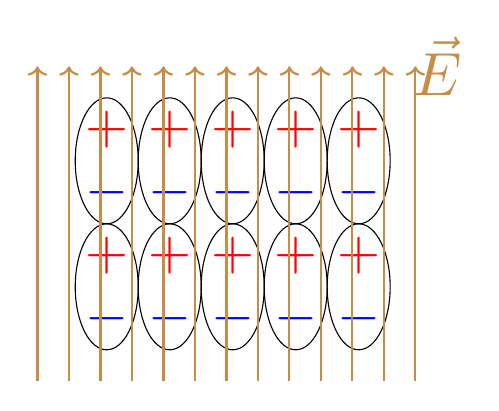
\begin{tikzpicture}[xscale=0.4,yscale=0.4]
    \draw[black] (-4,-2) ellipse (1 and 2);
    \node[blue] at (-4,-3) {$\Scale[2]{-}$};
    \node[red] at (-4,-1) {$\Scale[2]{+}$};
    \draw[black] (-4,2) ellipse (1 and 2);
    \node[blue] at (-4,1) {$\Scale[2]{-}$};
    \node[red] at (-4,3) {$\Scale[2]{+}$};
    \draw[black] (-2,-2) ellipse (1 and 2);
    \node[blue] at (-2,-3) {$\Scale[2]{-}$};
    \node[red] at (-2,-1) {$\Scale[2]{+}$};
    \draw[black] (-2,2) ellipse (1 and 2);
    \node[blue] at (-2,1) {$\Scale[2]{-}$};
    \node[red] at (-2,3) {$\Scale[2]{+}$};
    \draw[black] (0,-2) ellipse (1 and 2);
    \node[blue] at (0,-3) {$\Scale[2]{-}$};
    \node[red] at (0,-1) {$\Scale[2]{+}$};
    \draw[black] (0,2) ellipse (1 and 2);
    \node[blue] at (0,1) {$\Scale[2]{-}$};
    \node[red] at (0,3) {$\Scale[2]{+}$};
    \draw[black] (2,-2) ellipse (1 and 2);
    \node[blue] at (2,-3) {$\Scale[2]{-}$};
    \node[red] at (2,-1) {$\Scale[2]{+}$};
    \draw[black] (2,2) ellipse (1 and 2);
    \node[blue] at (2,1) {$\Scale[2]{-}$};
    \node[red] at (2,3) {$\Scale[2]{+}$};
    \draw[black] (4,-2) ellipse (1 and 2);
    \node[blue] at (4,-3) {$\Scale[2]{-}$};
    \node[red] at (4,-1) {$\Scale[2]{+}$};
    \draw[black] (4,2) ellipse (1 and 2);
    \node[blue] at (4,1) {$\Scale[2]{-}$};
    \node[red] at (4,3) {$\Scale[2]{+}$};
    \draw[GOLD_E, thick, ->] (-6.2,-5) -- (-6.2,5);
    \draw[GOLD_E, thick, ->] (-5.2,-5) -- (-5.2,5);
    \draw[GOLD_E, thick, ->] (-4.2,-5) -- (-4.2,5);
    \draw[GOLD_E, thick, ->] (-3.2,-5) -- (-3.2,5);
    \draw[GOLD_E, thick, ->] (-2.2,-5) -- (-2.2,5);
    \draw[GOLD_E, thick, ->] (-1.2,-5) -- (-1.2,5);
    \draw[GOLD_E, thick, ->] (-0.2,-5) -- (-0.2,5);
    \draw[GOLD_E, thick, ->] (0.8,-5) -- (0.8,5);
    \draw[GOLD_E, thick, ->] (1.8,-5) -- (1.8,5);
    \draw[GOLD_E, thick, ->] (2.8,-5) -- (2.8,5);
    \draw[GOLD_E, thick, ->] (3.8,-5) -- (3.8,5);
    \draw[GOLD_E, thick, ->] (4.8,-5) -- (4.8,5);
    \draw[GOLD_E, thick, ->] (5.8,-5) -- (5.8,5);
    \node[GOLD_E] at (6.5,5) {$\Scale[2.2]{\vec{E}}$};
\end{tikzpicture}
\label{fig:23:a}
\end{figure}
\end{flushleft}
\end{minipage}
~
\begin{minipage}{0.5\textwidth}
\begin{flushright}
\begin{figure}[H]
\captionsetup{width=0.8\textwidth,labelfont={color=black,bf},textfont={color=black}}
\centering
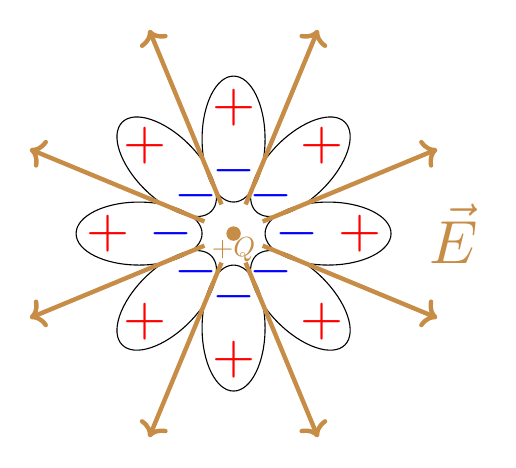
\begin{tikzpicture}[xscale=0.4,yscale=0.4]
    \filldraw [GOLD_E] (0,0) circle (6pt);
    \node[GOLD_E] at (0,-0.5) {$+Q$};
    \draw[black] (0,3) ellipse (1 and 2);
    \node[blue] at (0,2) {$\Scale[2]{-}$};
    \node[red] at (0,4) {$\Scale[2]{+}$};
    \draw[black] (3,0) ellipse (2 and 1);
    \node[blue] at (2,0) {$\Scale[2]{-}$};
    \node[red] at (4,0) {$\Scale[2]{+}$};
    \draw[black] (0,-3) ellipse (1 and 2);
    \node[blue] at (0,-2) {$\Scale[2]{-}$};
    \node[red] at (0,-4) {$\Scale[2]{+}$};
    \draw[black] (-3,0) ellipse (2 and 1);
    \node[blue] at (-2,0) {$\Scale[2]{-}$};
    \node[red] at (-4,0) {$\Scale[2]{+}$};
    \draw[black, rotate=45] (0,3) ellipse (1 and 2);
    \node[blue] at (1.2,1.2) {$\Scale[2]{-}$};
    \node[red] at (2.8,2.8) {$\Scale[2]{+}$};
    \draw[black, rotate=45] (0,-3) ellipse (1 and 2);
    \node[blue] at (-1.2,1.2) {$\Scale[2]{-}$};
    \node[red] at (-2.8,2.8) {$\Scale[2]{+}$};
    \draw[black, rotate=-45] (0,3) ellipse (1 and 2);
    \node[blue] at (-1.2,-1.2) {$\Scale[2]{-}$};
    \node[red] at (-2.8,-2.8) {$\Scale[2]{+}$};
    \draw[black, rotate=-45] (0,-3) ellipse (1 and 2);
    \node[blue] at (1.2,-1.2) {$\Scale[2]{-}$};
    \node[red] at (2.8,-2.8) {$\Scale[2]{+}$};
    \draw[GOLD_E, ultra thick, ->] (0.383,0.924) -- (2.679,6.467);
    \draw[GOLD_E, ultra thick, ->] (0.924,0.383) -- (6.467,2.679);
    \draw[GOLD_E, ultra thick, ->] (0.924,-0.383) -- (6.467,-2.679);
    \draw[GOLD_E, ultra thick, ->] (0.383,-0.924) -- (2.679,-6.467);
    \draw[GOLD_E, ultra thick, ->] (-0.383,0.924) -- (-2.679,6.467);
    \draw[GOLD_E, ultra thick, ->] (-0.924,0.383) -- (-6.467,2.679);
    \draw[GOLD_E, ultra thick, ->] (-0.924,-0.383) -- (-6.467,-2.679);
    \draw[GOLD_E, ultra thick, ->] (-0.383,-0.924) -- (-2.679,-6.467);
    \node[GOLD_E] at (7,0) {$\Scale[2.2]{\vec{E}}$};
\end{tikzpicture}
\label{fig:23:b}
\end{figure}
\end{flushright}
\end{minipage}

We also get local accumulations of charge that exist \underline{entirely} as a result of the polarizing field: bound charge (volume and surface). \\

In simple situations, $\bm{p} \propto \bm{E}$ $\left( \bm{p} = \epsilon_o\ \chi_e \bm{E} \right)$. As we discussed, many situations are not so simple. \\

Very much the same thing happens in magnetism. \\

Atomically, there are two places we find magnetic dipoles:

\begin{enumerate}

\item Intrinsic magnetic moments of elementary particles

An electron (like all fermions) has an intrinsic magnetic moment related to its intrinsic angular momentum, both of which are referred to as spin.

\begin{figure}[H]
\captionsetup{width=0.8\textwidth,labelfont={color=black,bf},textfont={color=black}}
\centering
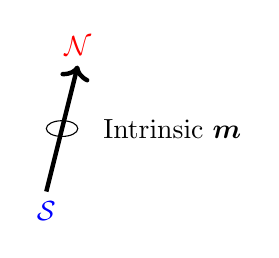
\begin{tikzpicture}[xscale=0.4,yscale=0.4]
    \draw[black, ultra thick, ->] (-0.5,-2) -- (0.5,2);
    \node[blue, below] at (-0.5,-2) {$\mathcal{S}$};
    \node[red, above] at (0.5,2) {$\mathcal{N}$};
    \draw[black] (0,0) ellipse (0.5 and 0.25);
    \node[black, right] at (1,0) {Intrinsic $\bm{m}$};
\end{tikzpicture}
\label{fig:23:c}
\end{figure}

I can give you no good reason as to why it exists. It simply does. The classical model of a spinning ball of charge falls apart under even the most casual prodding (see homework).

The spin magnetic moment of an electron is
\begin{equation*}
    \left| \bm{m}_e \right| = \frac{e\ \hbar}{2m} = \mu_B,
\end{equation*}

where $\mu_B$ is a unit of magnetic moment called the Bohr magnetron.

\item Orbital magnetic moments of atoms

There exist magnetic moments due to the interactions between electrons and nuclei. Classically we can think of this as because of the orbiting electron constituting a current, but this model also falls apart quickly

\begin{figure}[H]
\captionsetup{width=0.8\textwidth,labelfont={color=black,bf},textfont={color=black}}
\centering
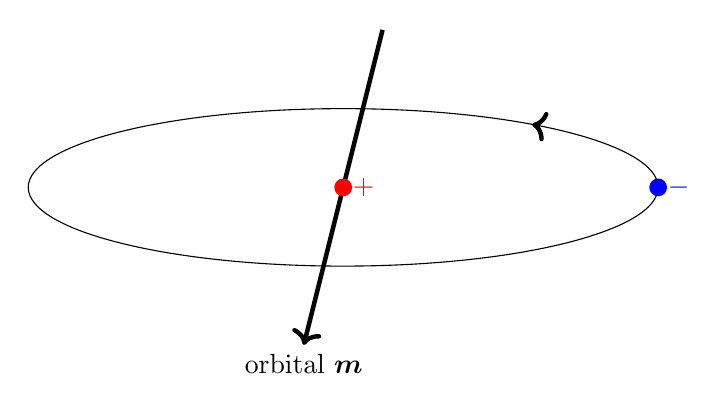
\begin{tikzpicture}[xscale=1,yscale=1]
    \draw[black, ultra thick, ->] (0.5,2) -- (-0.5,-2);
    \node[black, below] at (-0.5,-2) {orbital $\bm{m}$};
    \filldraw [red] (0,0) circle (3pt);
    \node[red, right] at (0,0) {$+$};
    \draw[black] (0,0) ellipse (4 and 1);
    \filldraw[blue] (4,0) circle (3pt);
    \node[blue, right] at (4,0) {$-$};
    \draw[black, ultra thick, ->] (2.5,0.781) -- (2.4,0.8);
\end{tikzpicture}
\label{fig:23:c}
\end{figure}

\end{enumerate}

However these atomic magnetic moments arise, they're usually randomly oriented and the overall average dipole moment per volume $\bm{M}$ (like magnetization) is zero.

But an applied magnetic field can align these dipoles, either with or against $\bm{B}$, and give us nonzero $\bm{M}$.

\begin{figure}[H]
\captionsetup{width=0.8\textwidth,labelfont={color=black,bf},textfont={color=black}}
\centering
\begin{tikzpicture}[xscale=1,yscale=1]
    \draw[black, thick, ->] (-4.48,-1.03) -- (-5.02,-1.5);
    \draw[black, thick, ->] (-4.25,-0.06) -- (-3.94,-0.64);
    \draw[black, thick, ->] (-3.57,0.68) -- (-3.1,1.05);
    \draw[black, thick, ->] (-2.72,0.54) -- (-2.46,-0.05);
    \draw[black, thick, ->] (-2.8,-0.53) -- (-3.39,-0.54);
    \draw[black, thick, ->] (-4.01,0.5) -- (-4.27,1.05);
    \draw[black, thick, ->] (-3.54,1.95) -- (-3.32,1.37);
    \draw[black, thick, ->] (-5.8,0.46) -- (-5.2,0.46);
    \node[ao] at (-4,-2.2) {no $\bm{B}$ applied};
    \node[black] at (-4,-2.7) {$\bm{m} = \bm{0}$};
    \node[black] at (0,0) {$\Scale[3]{\Longrightarrow}$};
    \draw[ao, ->] (5,-2) -- (5,3);
    \draw[ao, ->] (4,-2) -- (4,3);
    \draw[ao, ->] (3,-2) -- (3,3);
    \draw[ao, ->] (2,-2) -- (2,3);
    \draw[ao, ->] (6,-2) -- (6,3);
    \draw[black, thick, ->] (2.5,0.4) -- (2.5,1);
    \draw[black, thick, ->] (3.5,0.4) -- (3.5,1);
    \draw[black, thick, ->] (4.5,0.4) -- (4.5,1);
    \draw[black, thick, ->] (5.5,0.4) -- (5.5,1);
    \draw[black, thick, ->] (2.5,-0.6) -- (2.5,0);
    \draw[black, thick, ->] (3.5,-0.6) -- (3.5,0);
    \draw[black, thick, ->] (4.5,-0.6) -- (4.5,0);
    \draw[black, thick, ->] (5.5,-0.6) -- (5.5,0);
    \node[ao] at (4,-2.2) {$\bm{B}$ applied};
    \node[black] at (4,-2.7) {$\bm{m} \neq \bm{0}$};
\end{tikzpicture}
\label{fig:23:d}
\end{figure}

Generally,
\begin{equation*}
    \boxed{\bm{m} \propto \bm{B}}
\end{equation*}

We'll discuss the mechanisms by which this happens (paramagnetism, diamagnetism, ferromagnetism) later. For now we'll just accept that it can happen. \\

Recall that the vector potential due to a dipole of moment $\bm{m}$ is
\begin{equation*}
    \bm{A}(\bm{x}) = \frac{\mu_o}{4\pi} \frac{\bm{m} \times \bm{r}}{r^3}.
\end{equation*}

So if we have a function $\bm{M}(\bm{x})$ describing the volume density of the magnetic dipoles we can say
\begin{equation*}
    d\bm{A}(\bm{x}) = \frac{\mu_o}{4\pi} \frac{\bm{M} \times \bm{r}}{r^3} d^3x, \qquad \text{(with } d\bm{m} = \bm{M}d^3x \text{)}
\end{equation*}

This implies
\begin{gather*}
    \bm{A}(\bm{x}) = \frac{\mu_o}{4\pi} \int \frac{\bm{m}(\bm{x'}) \times \left( \bm{x} - \bm{x'} \right)\ d^3x'}{\left| \bm{x} - \bm{x'} \right|} \qquad\qquad\qquad \parbox[c]{0.4\linewidth}{This is general, but can be written in a more useful form using a derivation extremely similar to the one we did with $V(\bm{x})$ in chapter 6.}
\end{gather*}

We get

\begin{equation*}
    \bm{A}(\bm{x}) = \frac{\mu_o}{4\pi} \int \frac{\textcolor{ao}{\nabla' \times \bm{M}(\bm{x'})}\ d^3x'}{\left| \bm{x} - \bm{x'} \right|} + \frac{\mu_o}{4\pi} \int \frac{\textcolor{ORANGE}{\bm{M}(\bm{x'}) \times \nhat}\ dA'}{\left| \bm{x} - \bm{x'} \right|}.
\end{equation*}

Last chapter we derived
\begin{equation*}
    \bm{A}(\bm{x}) = \frac{\mu_o}{4\pi} \int \frac{\textcolor{ao}{\bm{J}(\bm{x'})}\ d^3x'}{\left| \bm{x} - \bm{x'} \right|} \qquad \text{and} \qquad \bm{A}(\bm{x}) = \frac{\mu_o}{4\pi} \int \frac{\textcolor{ORANGE}{\bm{K}(\bm{x'})}\ dA'}{\left| \bm{x} - \bm{x'} \right|}.
\end{equation*}

Comparing, we see these match up if \textcolor{ao}{$\bm{J}(\bm{x}) = \nabla \times \bm{M}(\bm{x'})$} and \textcolor{ORANGE}{$\bm{K}(\bm{x'}) = \bm{M}(\bm{x'}) \times \nhat$}. \\

Since these ``currents" only exist because of magnetization $\bm{M}$, we call them \textcolor{ao}{volume} and \textcolor{ORANGE}{surface} \underline{bound} currents. \\

Putting it all together, the $\bm{A}$ resulting from the $\bm{M}$ is 
\begin{equation*}
    \bm{A}(\bm{x}) = \frac{\mu_o}{4\pi} \int\limits_{\textcolor{ao}{\mathcal{V}}} \frac{\textcolor{ao}{\bm{J}_b}(\bm{x'})\ d^3x'}{\left| \bm{x} - \bm{x'} \right|} + \frac{\mu_o}{4\pi} \int\limits_{\textcolor{ORANGE}{\mathcal{A}}} \frac{\textcolor{ORANGE}{\bm{K}_b}(\bm{x'})\ dA'}{\left| \bm{x} - \bm{x'} \right|},
\end{equation*}

where the \textcolor{ao}{volume integral} is over the space filled by $\bm{M}$, and the \textcolor{ORANGE}{area integral} is over the area bounding that space.

\vspace{2cm}

\subsection*{Visualizing bound currents}

Classically, every magnetic dipole can be related back to a current loop, which we'll visualize as occupying a square unit cell.

\begin{figure}[H]
\captionsetup{width=0.8\textwidth,labelfont={color=black,bf},textfont={color=black}}
\centering
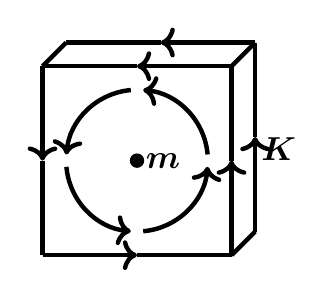
\begin{tikzpicture}[xscale=0.6,yscale=0.6]
    \draw[black, ultra thick, ->] (-2,-2) -- (0,-2);
    \draw[black, ultra thick] (0,-2) -- (2,-2);
    \draw[black, ultra thick, ->] (2,-2) -- (2,0);
    \draw[black, ultra thick] (2,0) -- (2,2);
    \draw[black, ultra thick, ->] (2,2) -- (0,2);
    \draw[black, ultra thick] (0,2) -- (-2,2);
    \draw[black, ultra thick, ->] (-2,2) -- (-2,0);
    \draw[black, ultra thick,] (-2,0) -- (-2,-2);
    \draw[black, ultra thick] (2,-2) -- (2.5,-1.5);
    \draw[black, ultra thick] (2,2) -- (2.5,2.5);
    \draw[black, ultra thick] (-2,2) -- (-1.5,2.5);
    \draw[black, ultra thick, ->] (2.5,-1.5) -- (2.5,0.5);
    \draw[black, ultra thick] (2.5,0.5) -- (2.5,2.5);
    \draw[black, ultra thick, ->] (2.5,2.5) -- (0.5,2.5);
    \draw[black, ultra thick] (0.5,2.5) -- (-1.5,2.5);
    \filldraw [black] (0,0) circle (4pt);
    \draw[black, ultra thick, ->] (1.49429,0.1307336) arc (5:85:1.5);
    \draw[black, ultra thick, ->] (-0.1307336,1.49429) arc (95:175:1.5);
    \draw[black, ultra thick, ->] (-1.49429,-0.1307336) arc (185:265:1.5);
    \draw[black, ultra thick, ->] (0.1307336,-1.49429) arc (275:355:1.5);
    \node[black] at (0.55,0) {$\Scale[1.2]{\bm{m}}$};
    \node[black] at (3,0.25) {$\Scale[1.2]{\bm{K}}$};
\end{tikzpicture}
\label{fig:23:tnt}
\end{figure}

Many cells together, assuming uniform $\bm{M}$, will result in a lot of cancellation and some leftover current on the perimeter (the bound surface current).

\begin{figure}[H]
\centering
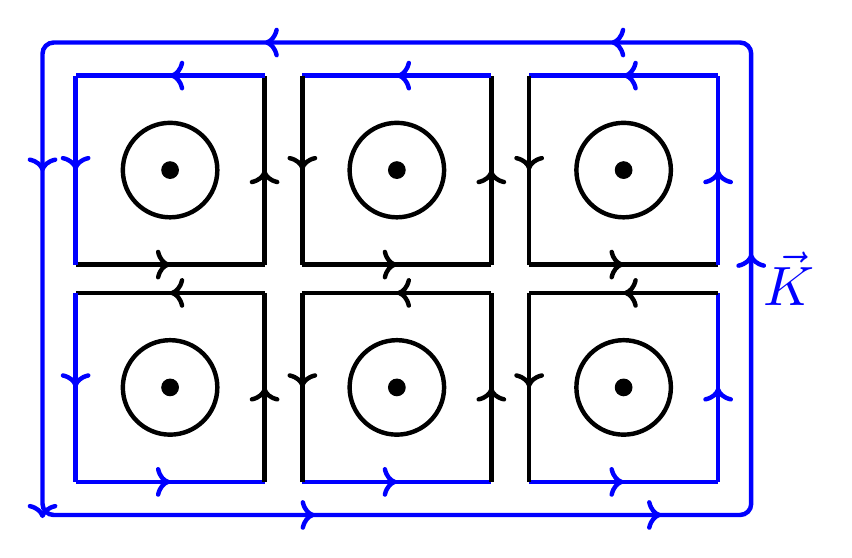
\begin{tikzpicture}[scale=0.6]

    % Bottom left
    \begin{scope}[shift={(-4.8,-2.3)}, decoration={markings, mark=at position 0.5 with {\arrow{>}}}]
    \draw[blue, ultra thick, postaction=decorate] (-2,-2) -- (2,-2);
    \draw[black, ultra thick, postaction=decorate] (2,-2) -- (2,2);
    \draw[black, ultra thick, postaction=decorate] (2,2) -- (-2,2);
    \draw[blue, ultra thick, postaction=decorate] (-2,2) -- (-2,-2);
    \draw[black, ultra thick] (0,0) circle (1);
    \filldraw[black] (0,0) circle (5pt);
    \end{scope}
    
    % Bottom center
    \begin{scope}[shift={(0,-2.3)}, decoration={markings, mark=at position 0.5 with {\arrow{>}}}]
    \draw[blue, ultra thick, postaction=decorate] (-2,-2) -- (2,-2);
    \draw[black, ultra thick, postaction=decorate] (2,-2) -- (2,2);
    \draw[black, ultra thick, postaction=decorate] (2,2) -- (-2,2);
    \draw[black, ultra thick, postaction=decorate] (-2,2) -- (-2,-2);
    \draw[black, ultra thick] (0,0) circle (1);
    \filldraw[black] (0,0) circle (5pt);
    \end{scope}
    
    % Bottom right
    \begin{scope}[shift={(4.8,-2.3)}, decoration={markings, mark=at position 0.5 with {\arrow{>}}}]
    \draw[blue, ultra thick, postaction=decorate] (-2,-2) -- (2,-2);
    \draw[blue, ultra thick, postaction=decorate] (2,-2) -- (2,2);
    \draw[black, ultra thick, postaction=decorate] (2,2) -- (-2,2);
    \draw[black, ultra thick, postaction=decorate] (-2,2) -- (-2,-2);
    \draw[black, ultra thick] (0,0) circle (1);
    \filldraw[black] (0,0) circle (5pt);
    \end{scope}
    
    % Top left
    \begin{scope}[shift={(-4.8,2.3)}, decoration={markings, mark=at position 0.5 with {\arrow{>}}}]
    \draw[black, ultra thick, postaction=decorate] (-2,-2) -- (2,-2);
    \draw[black, ultra thick, postaction=decorate] (2,-2) -- (2,2);
    \draw[blue, ultra thick, postaction=decorate] (2,2) -- (-2,2);
    \draw[blue, ultra thick, postaction=decorate] (-2,2) -- (-2,-2);
    \draw[black, ultra thick] (0,0) circle (1);
    \filldraw[black] (0,0) circle (5pt);
    \end{scope}
    
    % Top center
    \begin{scope}[shift={(0,2.3)}, decoration={markings, mark=at position 0.5 with {\arrow{>}}}]
    \draw[black, ultra thick, postaction=decorate] (-2,-2) -- (2,-2);
    \draw[black, ultra thick, postaction=decorate] (2,-2) -- (2,2);
    \draw[blue, ultra thick, postaction=decorate] (2,2) -- (-2,2);
    \draw[black, ultra thick, postaction=decorate] (-2,2) -- (-2,-2);
    \draw[black, ultra thick] (0,0) circle (1);
    \filldraw[black] (0,0) circle (5pt);
    \end{scope}
    
    % Top right
    \begin{scope}[shift={(4.8,2.3)}, decoration={markings, mark=at position 0.5 with {\arrow{>}}}]
    \draw[black, ultra thick, postaction=decorate] (-2,-2) -- (2,-2);
    \draw[blue, ultra thick, postaction=decorate] (2,-2) -- (2,2);
    \draw[blue, ultra thick, postaction=decorate] (2,2) -- (-2,2);
    \draw[black, ultra thick, postaction=decorate] (-2,2) -- (-2,-2);
    \draw[black, ultra thick] (0,0) circle (1);
    \filldraw[black] (0,0) circle (5pt);
    \end{scope}
    
    % Outer thingy
    \begin{scope}[decoration={markings, mark=between positions 0 and 1 step 4.4cm  with { \arrow[blue]{<};}}]
    \draw[blue, ultra thick, rounded corners, postaction=decorate] (-7.5, -5) rectangle (7.5, 5);
    \end{scope}
    
    % Label
    \node[blue] at (8.3,0) {$\Scale[2]{\vec{K}}$};
    
\end{tikzpicture}
\label{fig:23:f}
\end{figure}

If we have a nonuniform $\bm{M}$ --- probably (but not necessarily) coming from a nonuniform $\bm{B}$ --- we may end up with bound currents in the interior also.

\begin{figure}[H]
\captionsetup{width=0.8\textwidth,labelfont={color=black,bf},textfont={color=black}}
\centering
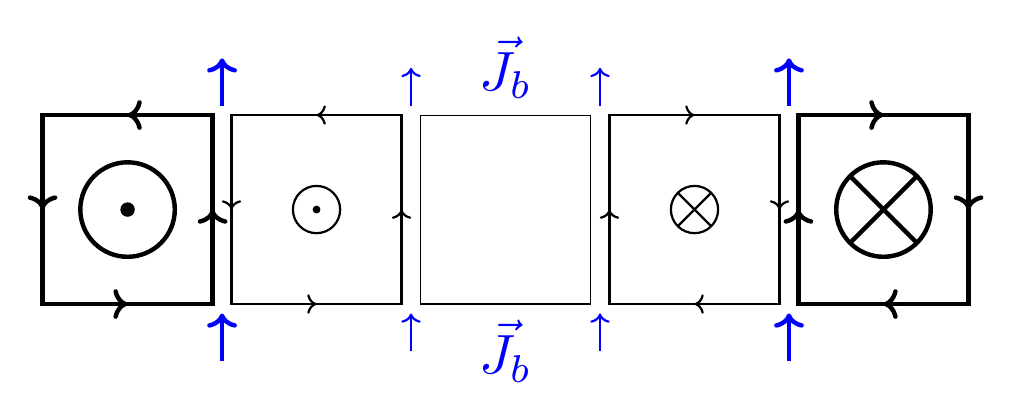
\begin{tikzpicture}[xscale=0.6,yscale=0.6]
    % Left-most
    \draw[black, ultra thick] (-9.8,-2) rectangle (-6.2,2);
    \filldraw [black] (-8,0) circle (4pt);
    \draw[black, ultra thick] (-8,0) circle (1);
    \draw[black, ultra thick, ->] (-9.8,2) -- (-9.8,0);
    \draw[black, ultra thick, ->] (-9.8,-2) -- (-8,-2);
    \draw[black, ultra thick, ->] (-6.2,-2) -- (-6.2,0);
    \draw[black, ultra thick, ->] (-6.2,2) -- (-8,2);
    % Left-center
    \draw[black, thick] (-5.8,-2) rectangle (-2.2,2);
    \filldraw [black] (-4,0) circle (2pt);
    \draw[black, thick] (-4,0) circle (0.5);
    \draw[black, thick, ->] (-5.8,2) -- (-5.8,0);
    \draw[black, thick, ->] (-5.8,-2) -- (-4,-2);
    \draw[black, thick, ->] (-2.2,-2) -- (-2.2,0);
    \draw[black, thick, ->] (-2.2,2) -- (-4,2);
    % Center
    \draw[black, thin] (-1.8,-2) rectangle (1.8,2);
    % Right-center
    \draw[black, thick] (2.2,-2) rectangle (5.8,2);
    \draw[black, thick] (4,0) circle (0.5);
    \draw[black, thick] (3.646,-0.354) -- (4.354,0.354);
    \draw[black, thick] (3.646,0.354) -- (4.354,-0.354);
    \draw[black, thick, ->] (5.8,2) -- (5.8,0);
    \draw[black, thick, ->] (5.8,-2) -- (4,-2);
    \draw[black, thick, ->] (2.2,-2) -- (2.2,0);
    \draw[black, thick, ->] (2.2,2) -- (4,2);
    % Right-most
    \draw[black, ultra thick] (6.2,-2) rectangle (9.8,2);
    \draw[black, ultra thick] (8,0) circle (1);
    \draw[black, ultra thick] (7.293,0.707) -- (8.707,-0.707);
    \draw[black, ultra thick] (7.293,-0.707) -- (8.707,0.707);
    \draw[black, ultra thick, ->] (9.8,2) -- (9.8,0);
    \draw[black, ultra thick, ->] (9.8,-2) -- (8,-2);
    \draw[black, ultra thick, ->] (6.2,-2) -- (6.2,0);
    \draw[black, ultra thick, ->] (6.2,2) -- (8,2);
    % Bottom arrows
    \draw[blue, ultra thick, ->] (-6,-3.2) -- (-6,-2.2);
    \draw[blue, thick, ->] (-2,-3) -- (-2,-2.2);
    \draw[blue, thick, ->] (2,-3) -- (2,-2.2);
    \draw[blue, ultra thick, ->] (6,-3.2) -- (6,-2.2);
    \node[blue] at (0,-3) {$\Scale[2]{\vec{J}_b}$};
    % Top arrows
    \draw[blue, ultra thick, ->] (-6,2.2) -- (-6,3.2);
    \draw[blue, thick, ->] (-2,2.2) -- (-2,3);
    \draw[blue, thick, ->] (2,2.2) -- (2,3);
    \draw[blue, ultra thick, ->] (6,2.2) -- (6,3.2);
    \node[blue] at (0,3) {$\Scale[2]{\vec{J}_b}$};
\end{tikzpicture}
\label{fig:23:g}
\end{figure}

\newpage

\section*{Lecture 24: $B$, $H$, and Boundary Conditions}
\setcounter{page}{1}

Let's briefly review how bound charge let to the idea of the displacement field $\bm{D}$. \\

The source equation $\nabla \cdot \bm{E} = \rho/\epsilon_o$ refers to \underline{all} charges, both free and bound:
\begin{equation*}
    \nabla \cdot \bm{E} = \frac{\rho_f + \rho_b}{\epsilon_o}
\end{equation*}

This is inconvenient, since we often can only specify the free charge. Since $\rho_b = -\nabla \cdot \bm{P}$, this invites some rearrangement:
\begin{equation*}
    \epsilon_o \left( \nabla \cdot \bm{E} \right) = \rho_f + \rho_b = \rho_f - \nabla \cdot \bm{P} \implies \nabla \cdot \left( \epsilon_o \bm{E} + \bm{P} \right) = \rho_f.
\end{equation*}

So, if we can define a composite field $\bm{D} \equiv \epsilon \bm{E} + \bm{P}$, we can recover a source equation in the style of Gauss's law, but written only in terms of free charge:
\begin{equation*}
    \nabla \cdot \bm{D} = \rho_f.
\end{equation*}

We're going to do something analogous for magnetism. Ampere's law says $\nabla \times \bm{B} = \mu_o \bm{J}$. That current density $\bm{J}$ is \underline{all} $\bm{J}$, free and bound:
\begin{equation*}
    \nabla \times \bm{B} = \mu_o \left( \bm{J}_f + \bm{J}_b \right).
\end{equation*}

Since $\bm{J}_b = \nabla \times \bm{M}$, we can do some reshuffling:
\begin{gather*}
    \nabla \times \frac{\bm{B}}{\mu_o} = \bm{J}_f + \nabla \times \bm{M} \\
    \implies \nabla \times \left( \frac{\bm{B}}{\mu_o} - \bm{M} \right) = \bm{J}_f,
\end{gather*}

Define $\bm{H} = \frac{\bm{B}}{\mu_o} - \bm{M}$ and we get
\begin{equation*}
    \boxed{\nabla \times \bm{H} = \bm{J}_f} \qquad \text{Ampere's Law in Matter}
\end{equation*}

\textbf{Interlude: }Naming $\bm{H}$ \& $\bm{B}$ (or, ``grumpy old people having a fight about stupid bullshit'') \\

So $\bm{E}$ is fundamental in that it is responsible for forces quite directly $\left( \bm{F} = q\bm{E} \right)$ and that  it is the field that gets produced by all charges, not just a special subset of charges $\left( \nabla \cdot \bm{E} = \rho_{\text{total}}/\epsilon_o \right)$. Thus, $\bm{E}$ is always the electric field, and the composite object $\bm{D}$ is given a special name, the displacement field. \\

Similarly, $\bm{B}$ is the field in the force law $\left( \bm{F} = q\bm{v} \times \bm{B} \right)$ and is the field produced by all forms of current. So obviously everyone calls $\bm{B}$ the magnetic field and $\bm{H}$ something else, right? \\

Ha ha. No. For some reason that I cannot find (and I've looked), some people call $\bm{B}$ the magnetic induction and $\bm{H}$ the magnetic field. And other people do other stuff.

\begin{table}[H]
\centering
\captionsetup{width=0.8\textwidth,labelfont={color=black,bf},textfont={color=black}}
\caption*{Names I've heard for $B$ and $H$}
\begin{tabular}{@{}c|c@{}}
\toprule
$\bm{B}$ & $\bm{H}$ \\ \midrule
Magnetic field & Magnetic field \\
Magnetic induction & Auxilary magnetic field \\
Magnetic flux density & Magnetic field strength \\ \bottomrule
\end{tabular}
\label{tab:23:names}
\end{table}

And people will fight to death over this sort of thing! We're going to keep it clean. $\bm{B}$ is the magnetic field. Period. And $\bm{H}$ we'll just call `H'. \\

Anyway, back to Ampere's law in matter:
\begin{equation*}
    \nabla \times \bm{H} = \bm{J}_f \qquad \text{or} \qquad \oint \bm{H} \cdot d\bm{\ell} = I_{f,\text{ enc}}.
\end{equation*}

Let's continue to parallel what was done for polarized dielectrics. There, $\bm{P} = \epsilon_o \chi_e \bm{E}$ for linear, isotropic materials and $\bm{D} = \epsilon \bm{E}$, with $\epsilon = \epsilon \left( 1 + \chi_e \right)$. Here, once again for linear isotropic materials, we define
\begin{align*}
    \bm{M} &= \chi_m \bm{H} \qquad \parbox[b]{0.5\linewidth}{($\chi_m$ is the magnetic susceptibility} \\
    \bm{B} &= \mu \bm{H} \qquad \parbox[b]{0.5\linewidth}{with $\mu = \mu_o\left( 1 + \chi_m \right)$; $\mu$ is named the `permeability'}
\end{align*}

$\chi_m$ is very small for almost all materials save ferromagnetic ones ($\chi_m \sim 10^{-3}$ --- $10^{-8}$). Thus for \underline{most} materials magnetization is much less relevant than polarization. \\

Also, we can derive an important constraint on $\bm{J}_b$ now: Since $\bm{J}_b = \nabla \times \bm{M}$, if $\bm{M} = \chi_m \bm{H}$, then
\begin{equation*}
    \bm{J}_b = \nabla \times \chi_m \bm{H} \qquad \text{and} \qquad \nabla \times \bm{H} = \bm{J}_f.
\end{equation*}

So
\begin{equation*}
    \boxed{\bm{J}_b = \chi_m \bm{J}_f} \qquad \parbox[c]{0.3\linewidth}{Therefore, if our material is linear, uniform, and isotropic, $\bm{J}_b$ can exist only if $\bm{J}_f$ exists.}
\end{equation*}

\subsection*{Boundary Conditions on $\bm{B}$ and $\bm{H}$}

We get these in the same way we got the conditions on $\bm{E}$ and $\bm{D}$. \\

$\nabla \cdot \bm{B} = 0$ is equivalent to $\displaystyle \oint \bm{B} \cdot d\bm{A} = 0$. So if we draw a small box around a surface and look at the flux through that box, only the flux through the top and the bottom matter if we make the box thin enough. And so,
\begin{equation*}
    \oint \bm{B} \cdot d\bm{A} = B_{\perp, \text{above}} A - B_{\perp, \text{below}} A = 0 \implies \boxed{B_{\perp, \text{above}} = B_{\perp, \text{below}}}
\end{equation*}

\underline{So the normal component of $\bm{B}$ is continuous across surfaces}. \\

$\nabla \times \bm{B} = \mu_o \bm{J}$ is equivalent to $\displaystyle \oint \bm{B} \cdot d\bm{\ell} = \mu_o I_{\text{enc}}$. \\

Draw an Amperian loop enclosing a surface and make it very thin. Crank out what we've done before. Then
\begin{gather*}
    B_{\parallel, \text{above}} L - B_{\parallel, \text{below}} L = \mu_o K L \\
    B_{\parallel, \text{above}} \cancel{L} - B_{\parallel, \text{below}} \cancel{L} = \mu_o K \cancel{L} \\
    \implies B_{\parallel, \text{above}} - B_{\parallel, \text{below}} = \mu_o K.
\end{gather*}

But we actually have to be a bit more careful this time, because only surface currents that pass through the loop count, which is to say only surface currents that are perpendicular to the loop face and thus to the parallel $B$ are being considered. \underline{Orientation matters}. We respect this by writing
\begin{equation*}
    \boxed{\bm{B}_{\parallel, 1} - \bm{B}_{\parallel, 2} = \mu_o \bm{K} \times \nhat}
\end{equation*}

where $\bm{n}$ is the normal vector to the surface. We're coming at this slightly back-ackwards. Instead of trying to write the component of $\bm{K}$ that goes through the loop, we're looking at the component of $\bm{K}$ that when crossed with $\nhat$ is parallel to the $B$'s under consideration. That is the component that matters. \\

For $\bm{H}$ it's much the same:
\begin{equation*}
    \nabla \cdot \bm{H} = \nabla \cdot \left( \frac{\bm{B}}{\mu_o} - \bm{M} \right) = 0
\end{equation*}

as long as $\nabla \cdot \bm{M} = 0$. This is usually true (it may be possible to rig an exception with ferromagnetic materials).
\begin{equation*}
    \text{So usually} \qquad \bm{H} \cdot \bm{H} = 0 \implies \boxed{H_{\perp, \text{above}} - H_{\perp, \text{below}} = 0}
\end{equation*}

\begin{equation*}
    \text{And } \nabla \times \bm{H} = \bm{J}_f \implies \boxed{H_{\parallel, 1} - H_{\parallel, 2} = \bm{K}_f \times \nhat}
\end{equation*}

\subsection*{Full boundary conditions (in statics) summarized}

\begin{table}[H]
\centering
\captionsetup{width=0.8\textwidth,labelfont={color=black,bf},textfont={color=black}}
\begin{tabular}{@{}c|c@{}}
\toprule
For $E$ & $E_{\perp, 1} - E_{\perp, 2} = \sigma/\epsilon_o$, $E_{\parallel}$ is continuous \\ \midrule
For $B$ & $B_{\perp}$ is continous, $B_{\parallel,1} - B_{\parallel,2} = \mu_o \bm{K} \times \nhat$ \\ \midrule
For $D$ & $D_{\perp,1} - D_{\perp,2} = \sigma_f$, $D_{\parallel}$ is continous if $\nabla \times \bm{P} = 0$ \\ \midrule
For $H$ & $H_{\perp}$ is continous if $\nabla \cdot \bm{M} = 0$. $H_{\parallel, 1} - H_{\parallel,2} = \bm{K}_f \times \nhat$ \\ \bottomrule
\end{tabular}
\label{tab:static_bcs}
\end{table}

You could memorize all of these and it wouldn't be a waste of time, but they all come from nearly identical derivations (one of two, anyway)

\begin{mdframed}[backgroundcolor=WHITE,align=center,userdefinedwidth=30em]

\begin{center}
    
$\nabla \cdot (\text{field})$ equations lead to conditions on $\text{field}_{\perp}$ \\

$\nabla \times (\text{field})$ equations lead to conditions on $\text{field}_{\parallel}$
    
\end{center}

\end{mdframed}

This is a mathematical and totally general result.

\newpage

\section*{Lecture 25: Examples, Including the Magnetic Scalar Potential}
\setcounter{page}{1}

One problem we've solved in the past is the electric field in a coaxial cable with a dielectric spacer. Let's solve the analogous problem in magnetics.

Take a coaxial cable. The interior wire has radius $a$. The return sheath has inner and outer radii $b$ and $c$, respectively. The gap is filled with an insulator with magnetic susceptibility $\chi_m$. The conductor has susceptibility $\chi_{mc}$.

\begin{figure}[H]
\centering
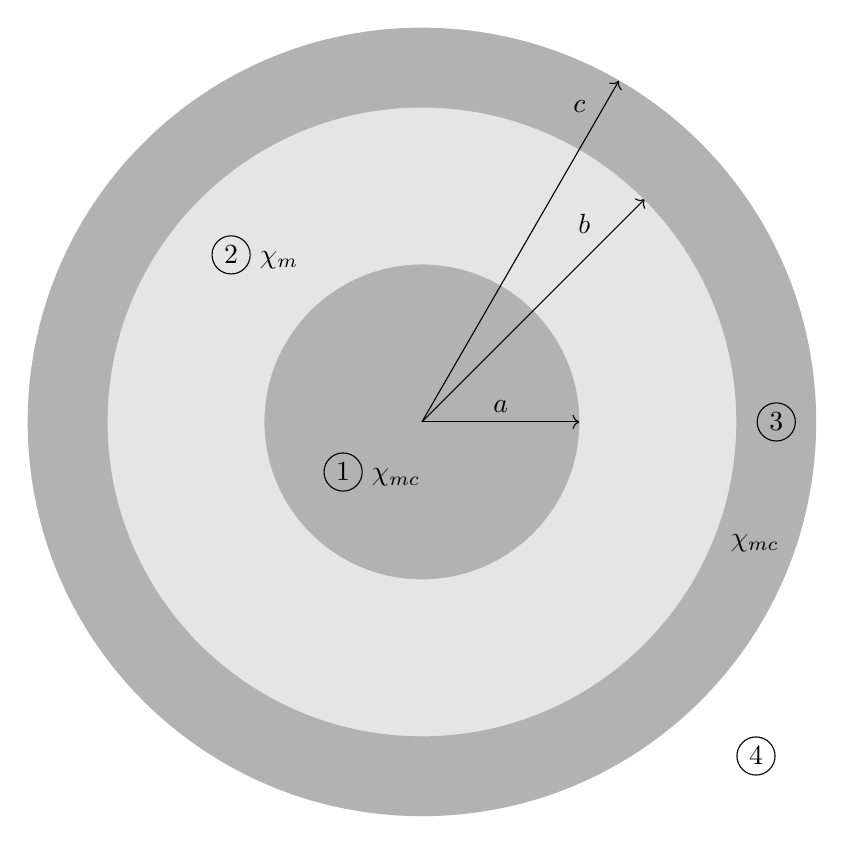
\begin{tikzpicture}
    \filldraw[black!30] (0,0) circle (2);
    \draw[black, ->] (0,0) -- (2,0) node[black, midway, above] {$a$};
    \fill[black!10, even odd rule] (0,0) circle[radius=4] circle[radius=2];
    \draw[black, ->] (0,0) -- (45:4) node[black, pos=0.8, anchor=south east] {$b$};
    \filldraw[black!30, even odd rule] (0,0) circle[radius=5] circle[radius=4];
    \draw[black, ->] (0,0) -- (60:5) node[black, pos=0.88, anchor=south east] {$c$};
    \node[black] at (225:0.9) {\circled{1}  $\chi_{mc}$};
    \node[black] at (135:3) {\circled{2}  $\chi_m$};
    \node[black] at (0:4.5) {\circled{3}};
    \node[black] at (-20:4.5) {$\chi_{mc}$};
    \node[black] at (-45:6) {\circled{4}};
\end{tikzpicture}
\label{fig:25a}
\end{figure}

If there's a current $I$, we have free current densities
\begin{equation*}
    \begin{cases} \displaystyle J_{f, \text{ in}} = \frac{I}{\pi a^2} (+\khat) & \text{for } r < a \\ \displaystyle J_{f, \text{ out}} = \frac{I}{\pi \left( c^2 - b^2 \right)} (-\khat) & \text{for } b < r < c \end{cases}
\end{equation*}

Note that the $\bm{J}$ vectors are in opposite directions.

We can't use $\nabla \times \bm{B} = \mu_o \bm{J}$, because $\bm{J}$ includes bound currents, so we instead work from $\nabla \times \bm{H} = \bm{J}_f$ or $\displaystyle \oint \bm{H} \cdot d\bm{\ell} = I_{f, \text{ enc}}$.

To find $\bm{H}$ we draw an Amperian loop in one of the four regions:

\begin{enumerate}

\item[\circled{1}] Inside the interior wire:

\begin{align*}
    \oint \bm{H} \cdot d\bm{\ell} = I_f &\implies H \left( 2\pi r \right) = J_{f, \text{ in}} \left( \pi r^2 \right) = \frac{I\ r^2}{a^2} \\
    &\implies \boxed{\bm{H} = \frac{I\ r}{2\pi a^2} \phihat, \qquad \text{for } r < a.}
\end{align*}

\item[\circled{2}] Inside the insulator:

Note that $I_{\text{enc}} = I$, so
\begin{align*}
    \boxed{\bm{H} = \frac{I}{2\pi r} \phihat, \qquad \text{for } a < r < b.}
\end{align*}

\item[\circled{3}] Inside the return sheath:

We enclose some current going in both directions, so
\begin{gather*}
    I_{\text{enc}} = I - J_{f, \text{ out}} \left( \pi r^2 - \pi b^2 \right) = I - \frac{I \left( r^2 - b^2 \right)}{c^2 - b^2} = I \left[ \frac{c^2 - b^2}{c^2 - b^2} - \frac{r^2 - b^2}{c^2 - b^2} \right] \\
    \implies \boxed{\bm{H} = \frac{I \left( c^2 - r^2 \right)}{2\pi r \left( c^2 - b^2 \right)} \phihat, \qquad \text{for } b < r < c.}
\end{gather*}

\item[\circled{4}] Outside the coaxial cable:

We now enclose all the current in both directions so $I_{\text{enc}} = 0$.
\begin{equation*}
    \implies \boxed{\bm{H} = \bm{0}, \qquad \text{for } r > c.}
\end{equation*}

\end{enumerate}

Note that throughout this problem we've been taking advantage of the cylindrical symmetry of the situation and the knowledge that $\bm{H}$ has to point in the $\phihat$ direction.

So let's find everything else. We know $\bm{B} = \mu \bm{H}$, so
\begin{equation*}
    \bm{B} = \begin{cases} \displaystyle \frac{\mu_o \left( 1 + \chi_{mc} \right) I r}{2\pi a^2} \phihat & \circled{1} \\[0.5cm] \displaystyle \frac{\mu_o \left( 1 + \chi_m \right) I}{2\pi r} \phihat & \circled{2} \\[0.5cm] \displaystyle \frac{\mu_o \left( 1 + \chi_{mc} \right) I \left( c^2 - r^2 \right)}{2\pi r \left( c^2 - b^2 \right)} \phihat & \circled{3} \\[0.5cm] \displaystyle 0 & \circled{4} \end{cases}
\end{equation*}

And the magnetization $\bm{M}$ is given by $\bm{M} = \chi \bm{H}$, so
\begin{equation*}
    \bm{M} = \begin{cases} \displaystyle \frac{\chi_{mc} I r}{2\pi a^2} \phihat & \circled{1} \\[0.5cm] \displaystyle \frac{\chi_m I}{2\pi r} \phihat & \circled{2} \\[0.5cm] \displaystyle \frac{\chi_{mc} I \left( c^2 - r^2 \right)}{2\pi r \left( c^2 - b^2 \right)} \phihat & \circled{3} \\[0.5cm] \displaystyle 0 & \circled{4} \end{cases}
\end{equation*}

We can get the bound current densities $\bm{J}_b$ and $\bm{K}_b$ from the magnetization $\bm{M}$. 

What should be the net bound current?

\subsection*{The magnetic scalar potential}

You may recall that $\nabla \times \bm{E} = \bm{0}$ implies $\displaystyle \oint \bm{E} \cdot d\bm{\ell} = 0$, which in turn implies that $\displaystyle \int \bm{E} \cdot d\bm{\ell}$ is path-independent and we can use it to build a scalar potential function $V$ such that $\bm{E} = -\nabla V$.

This doesn't work so well for the magnetic field since $\nabla \times \bm{B} = \mu_o \bm{J}$ and there's usually non-zero $\bm{J}$ if we're bothering to talk about $\bm{B}$. But there's a loophole.

We have that $\nabla \times \bm{H} = \bm{J}_f$ and sometimes $\bm{J}_f$ is zero when $\bm{J}_b$ isn't. So $\nabla \times \bm{B} \neq \bm{0}$ but $\nabla \times \bm{H} = \bm{0}$ and we have a legitimate situation where we can use a scalar potential for $\bm{H}$:
\begin{equation*}
    \bm{H} = -\nabla \phi_m \qquad \text{This works anytime } \bm{J}_f \text{ is zero.}
\end{equation*}

But why do we bother? What does this buy us? Well, $\nabla \cdot \bm{H} = \nabla \cdot \left( \mu \bm{B} \right)$. But Maxwell's equations tell us magnetic fields don't have divergence $\left( \nabla \cdot \bm{B} = 0 \right)$.  So if $\mu$ is spatially uniform,
\begin{gather*}
    \nabla \cdot \bm{H} = 0.
\end{gather*}

Substituting the scalar potential for $\bm{H}$, we get
\begin{equation*}
    \nabla^2 \phi_m = 0 \qquad {\parbox[c]{0.4\linewidth}{\begin{center} This is a good thing. We know all kinds of dirty tricks for solving this equation. \end{center}}}
\end{equation*}

As Pollack says, we can ``bring to bear'' the ``considerable mathematical armamentarium'' we have for such problems. In other words, we just made magnetostaics look like electrostatics (if $\bm{J}_f = 0$).

This really works, too. Check out an example:

A sphere of radius $a$ made of a material with susceptibility $chi_m$ is placed in a uniform magnetic field $\bm{B} = B_o \khat$.

There is no $\bm{J}_f$, so we can solve $\nabla^2 \phi_m = 0$ and go nuts. Which the book does. But you know what's better? \underline{We already solved this problem}.

Back in chapter 6 we did a polarizable sphere in a uniform $\bm{E}$-field. This is structurally identical. And what does a physicist do when they see a problem they've already solved? The write down the answer. From page 210:
\begin{equation*}
    \begin{cases} \displaystyle V_{\text{inside}} = -C_1 r \cos{\theta} \\[0.5cm] \displaystyle V_{\text{outside}} = -E_o r \cos{\theta} + \frac{C_2 a^3}{r^2} \cos{\theta} \end{cases} \quad \text{with} \quad C_1 = \left( \frac{3}{\kappa + 2} \right) E_o \quad \text{and} \quad C_2 = \left( \frac{\kappa + 1}{\kappa + 2} \right) E_o
\end{equation*}

Now we just fix it up a little. First off, $\kappa$ is the dielectric ``constant,'' $\displaystyle \kappa = \frac{\epsilon}{\epsilon_o}$. So we replace it with $\kappa_m = \frac{\mu}{\mu_o}$. And in electrostatics, $\bm{E = -\nabla V}$, but in magnetostatics, $\bm{H} = -\nabla \phi_m$. As such, we replace $E_o$ with $H_o$, \underline{not} $B_o$. Using $\displaystyle H_o = \frac{B_o}{\mu_o}$, we get
\begin{equation*}
    \phi_{m, \text{ in}} = \underbrace{\frac{-3 B_o}{\left( \kappa_m + 2 \right) \mu_o}}_{C_1} r\ \cos{\theta} \qquad \text{and} \qquad \phi_{m, \text{ out}} = \frac{-B_o r\ \cos{\theta}}{\mu_o} + \underbrace{\left( \frac{\kappa_{m} - 1}{\kappa_m + 2} \right) \frac{B_o}{\mu_o}}_{C_2} \frac{a^3\ \cos{\theta}}{r^2}.
\end{equation*}

Just like that. Now, there are some major \underline{physical} differences between electrostatics and magnetostatics. In the former, $\kappa \geqslant 1$ (always), but in the latter $\kappa_m$ can be less than 1.

Also, in electostatics, polarizing an object with $\kappa > 1$ leads to a charge separation that opposes the applied field. But in magnetostatics, magnetizing an object with $\kappa_m > 1$ enhances the applied field.

Let's see how this plays out in the above example for the interior electric and magnetic fields.

For the electric field, we have
\begin{equation*}
    V_{\text{inside}} = \frac{-3 E_o}{\kappa + 2} r\ \cos{\theta}.
\end{equation*}

Taking the negative gradient gives
\begin{align*}
    \bm{E}_{\text{inside}} &= -\frac{\partial V}{\partial r} \rhat - \frac{1}{r} \frac{\partial V}{\partial \theta} \thetahat \\
    &= \frac{3 E_o}{\kappa + 2} \cos{\theta}\ \rhat - \frac{3 E_o}{\kappa + 2} \sin{\theta}\ \thetahat
\end{align*}

Using $\khat = \cos{\theta}\ \rhat - \sin{\theta}\ \thetahat$ gives
\begin{equation*}
    \boxed{\bm{E}_{\text{inside}} = \frac{3 E_o}{\kappa + 2} \khat}
\end{equation*}

For the magnetic field, we know that
\begin{gather*}
    \bm{H}_{\text{inside}} = \frac{3 H_o}{\kappa_m + 2} \khat.
\end{gather*}

Using $\bm{B} = \mu \bm{H}$, we get
\begin{equation*}
    \underbrace{\frac{\bm{B}_{\text{inside}}}{\mu}}_{\bm{H_{\text{inside}}}} = \frac{3 \overbrace{\left( B_o / \mu_o \right)}^{H_o}}{\kappa_m + 2}\ \khat
\end{equation*}

Since $\displaystyle \kappa_m = \frac{\mu}{\mu_o}$,
\begin{equation*}
    \boxed{\bm{B}_{\text{inside}} = \frac{3 \kappa_m B_o}{\kappa_m + 2}\ \khat}
\end{equation*}

Sketching these out, we see.

Strongly diamagnetic materials significantly exclude applied $\bm{B}$-fields. Superconductors have $\kappa_m = 0$ and repel $\bm{B}$ completely, much as conductors have $\kappa \to \infty$ so that $\bm{E}_{\text{inside}} = \bm{0}$.

\textbf{Demo: } Pyrolytic graphite, a form of graphite that consists of sheets of graphene (planar arrangemetns of carbon atoms).

It is more diamagnetic at room temperature than any other known material.

A semi-classical explanation of this is that the carbon rings allow for strong induced currents when a $\bm{B}$-field is brought near. By Lenz's law, those currents will be in such a way as to create $\bm{B}$-fields that oppose the change in $\bm{B}$ that induced the currents, thereby leading to the possibility of levitation.

\subsection*{Magnetic Shielding}

I probably won't have to work very hard to convince you that sometimes you'll want to keep external magnetic fields away from certain objects or devices. Let's look at the principle of magnetic shielding.

Consider a \underline{spherical} shell of material with permeability $\mu$ and inner and outer radii $R_i$ and $R_o$, respectively.

We apply a magnetic field of the form $\bm{B} = B_o \khat$. There are no free currents, so we can define $\bm{H} = -\nabla \phi_m$. The external $\bm{H}$ is $\displaystyle \frac{\bm{B}}{\mu_o}$, so
\begin{equation*}
    \phi_{m, \text{ external}} = -\frac{B_o\ z}{\mu_o} = -\frac{B_o}{\mu_o} r\ \cos{\theta}.
\end{equation*}

We've solved problems like this before. Basically, we looked at the solution to $\nabla^2 V = 0$ in spherical and pulled out the terms proportional to $\cos{\theta}$. Those went like $r\ \cos{\theta}$ and $\displaystyle \frac{\cos{\theta}}{r^2}$.

For $r < R_i$, we exclude $\frac{\cos{\theta}}{r^2}$, since that blows up at $r = 0$:
\begin{equation*}
    \phi_{m, \text{ in}} (r, \theta) = \alpha r\ \cos{\theta}.
\end{equation*}

For $R_i < r < R_o$, we keep both terms:
\begin{equation*}
    \phi_{m, \text{ mid}} (r, \theta) = \gamma r\ \cos{\theta} + \frac{\delta\ \cos{\theta}}{r^2}.
\end{equation*}

For $r > R_o$, we know the $r\ \cos{\theta}$ term must match the applied potential at large $r$, so
\begin{equation*}
    \phi_{m, \text{ out}} (r, \theta) = -\frac{B_o}{\mu_o} r\ \cos{\theta} + \beta \frac{\cos{\theta}}{r^2}
\end{equation*}

In summary:
\begin{equation*}
    \phi_m = \begin{cases} \displaystyle \alpha r\ \cos{\theta} & r < R_i \\[0.5cm] \displaystyle \gamma r\ \cos{\theta} + \frac{\delta\ \cos{\theta}}{r^2} & R_i < r < R_o \\[0.5cm] \displaystyle -\frac{B_o}{\mu_o} r\ \cos{\theta} + \beta \frac{\cos{\theta}}{r^2} & r > R_o \end{cases}
\end{equation*}

Four constants to find: $\alpha$, $\beta$, $\gamma$, and $\delta$. We need to invoke four boundary conditions. There are many possible choices; as always there's a bit of an art to choosing easy ones. I, for one, like to use the continuity of the potential whenever possible. The book seems to agree.
\begin{gather*}
    \phi_{m, \text{ in}} (R_i) = \phi_{m, \text{ mid}} (R_i) \implies \alpha R_i = \gamma R_i + \frac{\delta}{R_i^2} \\
    \phi_{m, \text{ mid}} (R_o) = \phi_{m, \text{ out}} (R_o) \implies \gamma R_o + \frac{\delta}{R_o^2} = -\frac{B_o}{\mu_o} + \frac{B_o}{R_o^2}
\end{gather*}

And we can get two more equations from the continuity of $B_{\perp}$:
\begin{gather*}
    \mu_o \frac{\partial \phi_{m, \text{ in}} (R_i)}{\partial r} = \mu \frac{\partial \phi_{m, \text{ mid}} (R_i)}{\partial r} \qquad \text{and} \qquad \mu_o \frac{\partial \phi_{m, \text{ mid}} (R_o)}{\partial r} = \mu \frac{\partial \phi_{m, \text{ out}} (R_o)}{\partial r}
\end{gather*}

We end up with four linear equations in four unknowns. Matrix mojo ensues. The complete list of coefficients is in the book. We'll just look at $\alpha$ since its pertinent to $B_{\text{inside}}$:

For large $\kappa_m$, the denominator is proportional to

The more permeable the material, the weaker the field in the shielded region. There exist materials engineered to have very high $\kappa_m$, such as the alloy $\mu$-meta (Fe, Ni, Cu, Cr), with $\kappa_m$ up to $10^5$.

Note that this has applications not just in keeping $\bm{B}$-fields out of a place, but also in getting them from one place to another (see transformer design, for example).

\newpage

\section*{Lecture 26: Diamagnetism, Paramagnetism, and Ferromagnetism}
\setcounter{page}{1}

\newpage

\section*{Lecture 27: Motional EMF and Faraday's Law I}
\setcounter{page}{1}

\epigraph{``Mr. Faraday, of what use are your discoveries?'' \\ ``Madam, of what use is a baby?''}{Michael Faraday}

We're now moving into full-blown electrodynamics, where there will almost always be some time-dependence somewhere. We need to start with a little vocabulary:

\begin{mdframed}[backgroundcolor=WHITE,align=left,userdefinedwidth=45em, topline=false, rightline=false,frametitle={Electromotive Force (emf)}]

A measure of how much work a system is doing on a unit charge. Has units of volts (V), (energy/charge).

Physically, very much like voltage, though ``voltage'' or ``electric potential'' tends to be used in situations where a scalar potential can be defined.

\end{mdframed}

Since work is $\displaystyle \int \bm{F} \cdot d\bm{\ell}$ and the Lorentz force law is $\displaystyle \bm{F} = q \left( \bm{E} + \bm{v} \times \bm{E} \right)$, emf will be of the form $\displaystyle \int \frac{\bm{F}}{q} \cdot d\bm{\ell} = \int \left( \bm{E} + \bm{v} \times \bm{B} \right) \cdot d\bm{\ell}$. Generally, we will focus on either electric or magnetic forces. We've seen Faraday's law written two different ways in Phys 200:
\begin{equation*}
    \oint \left( \bm{E} + \bm{v} \times \bm{B} \right) \cdot d\bm{\ell} = -\frac{d}{dt} \int \bm{B} \cdot d\bm{A} \qquad \text{and} \qquad \mathcal{E} = -\frac{d \Phi}{dt}
\end{equation*}

And we're going to add a thrid:
\begin{equation*}
    \nabla \times \bm{E} = -\frac{\partial \bm{B}}{\partial t}
\end{equation*}


Let's work through a few different situations and see what kind of insight we can obtain.

\subsection*{EMF from a static $\bm{B}$-field}

Let's suppose we have a $\bm{B}$-field that occupies some region of space. It's uniform, with magnitude $B$, into the page. Everywhere else $B$ is zero. (This field is actually unphysical --- do you see why?)

We also have a wire loop with dimensions $W$ and $L$ partially in the field. We're pulling it out with some speed $v$.

\begin{figure}[H]
\centering
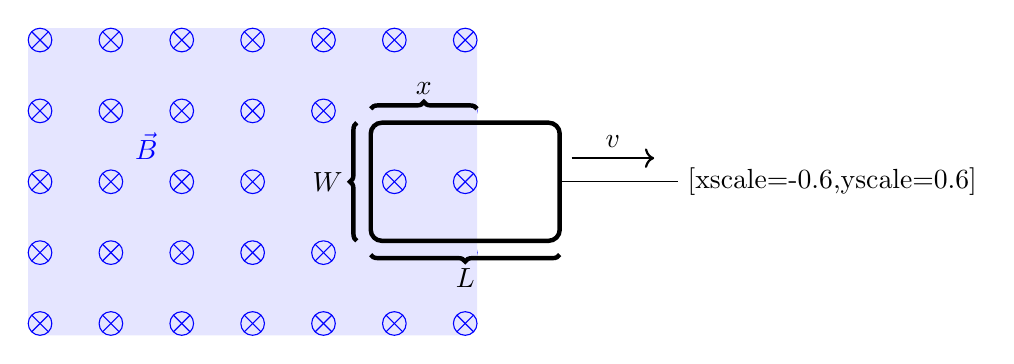
\begin{tikzpicture}[scale=0.15]
    
    \fill[blue!10, rounded corners] (-19, -13) rectangle (19, 13);
    
    \node[blue] at (-9,3) {$\vec{B}$};

    \foreach \x in {-18, -12, -6, 0, 6, 12, 18}
    \foreach \y in {-12, -6, 0, 6, 12}
    {
    \begin{scope}[shift={(\x,\y)}]
        \draw[blue] (0,0) circle (1);
        \draw[blue] (45:1) -- (225:1);
        \draw[blue] (135:1) -- (315:1);
    \end{scope}
    }
    
    \fill[blue!10] (4,-2) rectangle (8,2);
    
    \fill[blue!10] (10,4) rectangle (14,8);
    \fill[blue!10] (16,4) rectangle (19,8);
    
     \fill[blue!10] (10,-4) rectangle (14,-8);
    \fill[blue!10] (16,-4) rectangle (19,-8);
    
    
    \draw[black, ultra thick, rounded corners] (10,-5) rectangle (26,5);
    \draw[black] (26,0) -- (36,0) node[black, right]{\okay[xscale=-0.6,yscale=0.6]};
    \draw[black, thick, ->] (27,2) -- (34,2) node[black, midway, above] {$v$};
    
    \draw[black, ultra thick, decoration={brace, mirror, raise=5pt}, decorate] (10,-5) -- (26,-5) node[black, midway, below=6pt] {$L$};
    \draw[black, ultra thick, decoration={brace, raise=5pt}, decorate] (10,-5) -- (10,5) node[black, midway, left=6pt] {$W$};
    \draw[black, ultra thick, decoration={brace, raise=5pt}, decorate] (10,5) -- (19,5) node[black, midway, above=6pt] {$x$};
    
\end{tikzpicture}
\label{fig:27:loop}
\end{figure}

The charge carriers in the wires (let's call them positive for convenience) feel an emf due to the Lorenz force:
\begin{equation*}
    \mathcal{E} = \oint \left( \bm{v} \times \bm{B} \right) \cdot d\bm{\ell} \qquad \parbox[c]{0.5\linewidth}{Now, the right-hand-rule shows us that only charges in the leftmost wire segment are acted on (only there is $\bm{v} \times \bm{B}$ parallel to $d\bm{\ell}$.}
\end{equation*}

This implies
\begin{equation*}
    \mathcal{E} = vBW.
\end{equation*}

Let's look at the change in magnetic flux, $\displaystyle \frac{d \Phi}{dt}$, also. Note that $\displaystyle \Phi = \int \bm{B} \cdot d\bm{A}$, or in this case, $\Phi = BWx$. Thus
\begin{equation*}
    \frac{d \Phi}{dt} = \frac{d}{dt} \left( B W x \right) = B W \underbrace{\frac{d x}{dt}}_{\displaystyle v}
\end{equation*}

So we find that
\begin{equation*}
    \boxed{\mathcal{E} = \oint \left( \bm{v} \times \bm{B} \right) \cdot d\bm{\ell} = -\frac{d \Phi}{dt}}
\end{equation*}

(What's that sign about?)

You'll notice there is \underline{no $\bm{E}$ anywhere} in the problem.

This turns out to be a general result for \underline{any} moving loop in a $\bm{B}$-field. You can prove it using $\nabla \cdot \bm{B} = 0$ and $\bm{F} = q\bm{v} \times \bm{B}$. To emphasize for future use:
\begin{mdframed}[backgroundcolor=WHITE,align=center,userdefinedwidth=20em]
\begin{gather*}
    \nabla \cdot \bm{B} = 0 \qquad \text{and} \qquad \bm{F} = q\bm{v} \times \bm{B} \\
    \implies \mathcal{E} = -\frac{d \Phi}{dt}
\end{gather*}
\end{mdframed}

With no electric field, and being derivable from existing principles, this is \underline{not} Faraday's Law (not when the emf comes from a strictly magnetic force). But it is quite closely related. And you'll get the same answers for straight wire, no loop.

\subsection*{Electromagnetic Induction and Faraday's (actual) Law}

Now, what of the reciprocal situation where the wire loop is stationary and the region occupied by the field is moving, thereby providing a time-varying $\bm{B}$-field?

\begin{figure}[H]
\centering
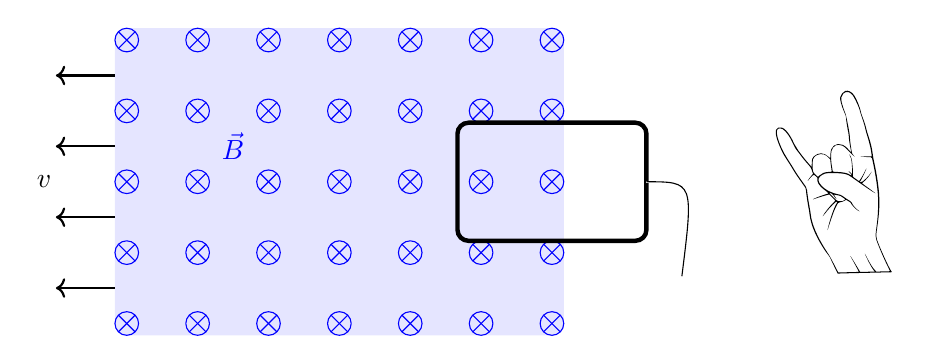
\begin{tikzpicture}[scale=0.15]
    
    \fill[blue!10, rounded corners] (-19, -13) rectangle (19, 13);
    
    \node[blue] at (-9,3) {$\vec{B}$};

    \foreach \x in {-18, -12, -6, 0, 6, 12, 18}
    \foreach \y in {-12, -6, 0, 6, 12}
    {
    \begin{scope}[shift={(\x,\y)}]
        \draw[blue] (0,0) circle (1);
        \draw[blue] (45:1) -- (225:1);
        \draw[blue] (135:1) -- (315:1);
    \end{scope}
    }
    
    \draw[black, ultra thick, rounded corners] (10,-5) rectangle (26,5);
    \draw[white,thick] (26,0) -- (36,0) node[black, right]{\rockandroll[scale=1]};
    \draw (26,0) .. controls (30,0) .. (29,-8);
    
    \foreach \z in {-9, -3, 3, 9}
    {
    \draw[black, thick, ->] (-19,\z) -- (-24, \z);
    }
    \node[black] at (-25, 0) {$v$};
    
\end{tikzpicture}
\label{fig:27:region}
\end{figure}

We cannot derive what happens from what we currently know. We need a brand new, empirically obtained law. Enter Faraday's law in differential form:
\begin{equation*}
    \boxed{\nabla \times \bm{E} = -\frac{\partial \bm{B}}{\partial t}} \qquad \parbox[c]{0.5\textwidth}{This law tells us that $E$-fields have another source besides charges: time-varying magnetic fields}
\end{equation*}

This law will let us figure out what happens in any situation where the magnetic field is changing, thus inducing a curly emf such that
\begin{equation*}
    \oint \bm{E} \cdot d\bm{\ell} \neq 0 \qquad \text{And so we come full circle.}
\end{equation*}

We have to proceed carefully, though. Many people (and books) screw up what follows as we try to get Faraday's law into integral form. First, integrate both sides over some \underline{open} surface:
\begin{align*}
    \int \left( \nabla \times \bm{E} \right) \cdot d\bm{A} = -\int \frac{\partial \bm{B}}{\partial t} \cdot d\bm{A} && \parbox[c]{0.4\textwidth}{Apply Stokes Theorem on the left} \\
    \oint \bm{E} \cdot d\bm{\ell} = -\int \frac{\partial \bm{B}}{\partial t} \cdot d\bm{A} && \parbox[c]{0.4\textwidth}{Right-hand side is a spatial integral only, so we can pull out $\frac{\partial}{\partial t}$ and make it a total derivative} \\
    \boxed{\oint \bm{E} \cdot d\bm{\ell} = -\frac{d}{dt} \int \bm{B} \cdot d\bm{A}}
\end{align*}

That seemed simple enough. And it's true that $\displaystyle \nabla \times \bm{E} = -\frac{\partial \bm{B}}{\partial t}$ and $\displaystyle \oint \bm{E} \cdot d\bm{\ell} = -\frac{d}{dt} \int \bm{B} \cdot d\bm{A}$ are equivalent \underline{if and only if} $\bm{B}$ is the \underline{only} thing with a time dependence.

What happens if we go back to the first situation, where the magnetic field isn't changing but the loop is moving? Start with:
\begin{align*}
    \nabla \times \bm{E} = -\frac{\partial \bm{B}}{\partial t} && \parbox[c]{0.4\textwidth}{Integrate both sides and apply Stokes' Theorem on the left} \\
    \oint \bm{E} \cdot d\bm{\ell} = -\int \frac{\partial \bm{B}}{\partial t} \cdot d\bm{A} && \parbox[c]{0.4\textwidth}{Now we \underline{don't} pull out $\frac{\partial}{\partial t}$. Why not?}
\end{align*}

So what we have here is that $\displaystyle \nabla \times \bm{E} = -\frac{\partial \bm{B}}{\partial t}$ and the above \underline{are} equivalent with no restrictions whatsoever. But we can't necessarily get that $\displaystyle \frac{\partial}{\partial t}$ out if the area is changing, because the \underline{bounds} of the integral are time dependent!

\begin{equation*}
    \oint \bm{E} \cdot d\bm{\ell} = -\int\limits_{s(t)} \frac{\partial \bm{B}}{\partial t} \cdot d\bm{A} \qquad \parbox[c]{0.4\textwidth}{\circled{2} Note that this does give a consistent result in the case of the moving loop, since $\frac{\partial \bm{B}}{\partial t} = 0$ and $\bm{E} = 0$ there.}
\end{equation*}

But can we do better? What can we do with that $\displaystyle \int \frac{\partial \bm{B}}{\partial t} \cdot d\bm{A}$ term? Let's look at
\begin{equation*}
    -\frac{d}{dt} \int\limits_{s(t)} \bm{B} \cdot d\bm{A}
\end{equation*}

and see if we can relate it. You take the derivative of functions whose bounds have variables using the Leibniz rules. You've seen one in one-dimension:
\begin{equation*}
    \frac{d}{dt} \int_{a(t)}^{b(t)} f(x, t)\ dx = \frac{d b}{dt} f(b, t) - \frac{d a}{dt} f(a, t) + \int_a^b \frac{\partial}{\partial t} f(x, t)\ dx.
\end{equation*}

It's got a vaguely product/chain rule flavor to it, where to apply the derivative completely, we need to hit the $b$-endpoint, the $a$-endpoint and the integrand. This generalizes to to vector fields instead of scalar functions, but not cleanly. Letting $\bm{B}$ be our vector field, the three-dimensional Leibniz rule gives:
\begin{equation*}
    \frac{d}{dt} \int \bm{B}(\bm{x}, t) \cdot d\bm{A} = \int \left( \frac{\partial \bm{B}}{\partial t} + \left( \nabla \cdot \bm{B} \right) \bm{v} \right) \cdot d\bm{A} - \oint \left( \bm{v} \times \bm{B} \right) \cdot d\bm{\ell},
\end{equation*}

where $\bm{v}$ comes from the time derivative of the spatial coordinates defining the are (so, for example, the velocity of the wire loop). Recall that $\nabla \cdot \bm{B} = 0$, so we can find that
\begin{equation*}
    -\int \frac{\partial \bm{B}}{\partial t} \cdot d\bm{A} = -\oint \left( \bm{v} \times \bm{B} \right) \cdot d\bm{\ell} - \frac{d}{dt} \int \bm{B}(\bm{x}, t) \cdot d\bm{A}
\end{equation*}

Substituting this into \circled{2} yields
\begin{gather*}
    \oint \bm{E} \cdot d\bm{\ell} = -\oint \left( \bm{v} \times \bm{B} \right) \cdot d\bm{\ell} - \frac{d}{dt} \int \bm{B} \cdot d\bm{A} \\
    \implies \boxed{\oint \left( \bm{E} + \bm{v} \times \bm{B} \right) \cdot d\bm{\ell} = -\frac{d}{dt} \int \bm{B} \cdot d\bm{A}}
\end{gather*}

Which is true \underline{generally}. It's basically a version of $\displaystyle \mathcal{E} = -\frac{d\Phi}{dt}$ that shows explicitly how $\bm{E}$ and $\bm{B}$ can \underline{both} contribute to the emf.

\begin{table}[H]
\centering
\captionsetup{width=0.8\textwidth,labelfont={color=black,bf},textfont={color=black}}
\caption*{Five forms of Faraday's law}
\begin{tabular}{@{}c|c@{}}
\toprule
\parbox[c]{0.3\textwidth}{\begin{equation*}
    \nabla \times \bm{E} = -\frac{\partial \bm{E}}{\partial t}
\end{equation*}} & \parbox[c]{0.5\textwidth}{\begin{center}
    Faraday's law proper, in differential form. Relates time-varying $\bm{B}$-fields and curly $\bm{E}$-fields at single points in space.
\end{center}} \\ \midrule
\parbox[c]{0.3\textwidth}{\begin{equation*}
    \oint \bm{E} \cdot d\bm{\ell} = -\int \frac{\partial \bm{B}}{\partial t} \cdot d\bm{A}
\end{equation*}} & \parbox[c]{0.5\textwidth}{\begin{center}
    Integral form of the above. Always true. Relates $\bm{E}$ and $\bm{B}$ over entire regions.
\end{center}} \\ \midrule
\parbox[c]{0.3\textwidth}{\begin{equation*}
    \oint \bm{E} \cdot d\bm{\ell} = -\frac{d}{dt} \int \bm{B} \cdot d\bm{A}
\end{equation*}} & \parbox[c]{0.5\textwidth}{\begin{center}
    True \underline{only} if the loop in question is entirely static. If misapplied generally, forces you to conclude that there's a curly $\bm{E}$-field present \underline{anytime} there's a time-varying flux for any reason. This can lead to some serious substantive errors - it's note mere pedantry.
\end{center}} \\ \midrule
\parbox[c]{0.4\textwidth}{\begin{equation*}
    \oint \left( \bm{E} + \bm{v} \times \bm{B} \right) \cdot d\bm{\ell} = -\frac{d}{dt} \int \bm{B} \cdot d\bm{A}
\end{equation*}} & \parbox[c]{0.5\textwidth}{\begin{center}
    Corrected form of the above. Adding a motional emf term fixes it.
\end{center}} \\ \midrule
\parbox[c]{0.3\textwidth}{\begin{equation*}
    \mathcal{E} = -\frac{d\Phi}{dt}
\end{equation*}} & \parbox[c]{0.5\textwidth}{\begin{center}
    A field-agnostic version of ``Faraday's law.'' Says that time-varying magnetic fluxes are associated with voltages. Doesn't actually say time-varying $\bm{B}$-fields have anything to do with curly $\bm{E}$-fields. So is it really Faraday's law? Seems like ``Faraday's law'' has evolved into kind of an umbrella term. And that's okay, if you understand the bits and pieces.
\end{center}} \\ \bottomrule
\end{tabular}
\label{tab:27:five}
\end{table}

\newpage

\section*{Lecture 28: Denouement}
\setcounter{page}{1}

\newpage

\end{document}